\documentclass[12pt, letterpaper]{report}

\usepackage{pucv_inf_2024}

% Holgura tipografica adicional: evita lineas desbordadas en parrafos con
% terminos tecnicos largos y en las entradas de bibliografia con DOI.
\emergencystretch=2em
\hyphenpenalty=100
\tolerance=1500

% Localizacion de los rotulos que la plantilla deja en ingles.
\renewcommand{\figurename}{Figura}
\renewcommand{\tablename}{Tabla}
\renewcommand{\chaptername}{Capítulo}
\renewcommand{\appendixname}{Anexo}

\title{Diseño y evaluación de arquitecturas de optimización basadas en metaheurísticas para sistemas híbridos de energías renovables con tecnologías de hidrógeno verde}
\author{Luciano Oliva}
\date{Marzo 2026}

\addbibresource{refs/referencias.bib}

\begin{document}

\begin{titlepage}
  \addtocounter{page}{-1}
  \thispagestyle{plain}

  \makeatletter
  \begin{picture}(0,0)
    \put(-75,-80){
\includegraphics[width=20cm]{assets/encabezado.png}}
  \end{picture}

  \begin{flushright}
    \vspace*{\fill}

    {\textcolor{titlecolor}{\LARGE\bfseries\MakeUppercase{\@title}}}

    \vspace*{\fill}

    {\textcolor{titlecolor}{\Large\bfseries\textsc{\@author}}}

    \vspace{1cm}

    {\textcolor{titlecolor}{\bfseries\textsc{
      Seminario de Proyectos\\[0.2cm]
      \@date
    }}}
  \end{flushright}
  \makeatother
\end{titlepage}


\chapter*{Resumen}
\addcontentsline{toc}{chapter}{Resumen}
\noindent

El dimensionamiento de sistemas híbridos eólico--fotovoltaico--electrolizador--batería es un problema de optimización de caja negra: cada diseño requiere una simulación horaria secuencial y la restricción sobre la energía vendida a la red sólo puede verificarse al finalizar el año. Esta tesis desarrolla un marco reproducible para comparar metaheurísticas clásicas e híbridas sobre ese problema, con el costo nivelado de la energía (LCOE) como única función objetivo. El costo presente neto y el costo nivelado del hidrógeno según esta tesis se reportan como indicadores secundarios.

Primero se reconstruye el modelo WPEB de Li et al. \cite{Li2024WPEB}; la comparación mediante errores absolutos y relativos sustenta una reproducción parcial, no una equivalencia exacta. Después se formula el problema como la minimización del LCOE sobre un dominio mixto, con capacidad eólica continua y catálogos discretos para electrolizador y batería, y se definen ocho instancias que varían el límite de ventas a red, la finura de los catálogos y la escala de la planta. Cada instancia se resuelve además por fuerza bruta sobre el dominio discretizado a 0,01 MW, entre \BFEDesigns{} y \BFCDesigns{} diseños anuales, lo que proporciona un óptimo exacto como referente de todas las brechas.

Se comparan siete algoritmos con presupuesto idéntico de \RequestsPerRun{} solicitudes y \Replicates{} ejecuciones independientes por instancia: cinco metaheurísticas clásicas (GWO, PSO, GA, SHO y WOA), un híbrido integrativo de bajo nivel (PSO+GA), construido sin alterar la implementación de los métodos de los que parte, y la búsqueda aleatoria como línea base. La comparación sigue un protocolo estadístico de siete pasos con contrastes bilaterales, nivel de significación y tolerancia práctica fijados antes de ejecutar las cuatro últimas instancias, que separa tres preguntas: en una instancia, Mann--Whitney sobre las ejecuciones; en general, Wilcoxon de rangos con signo sobre una mediana por instancia; y para los siete a la vez, Friedman con la corrección de Iman--Davenport. Las diferencias se cuantifican con el tamaño de efecto $\hat{A}_{12}$ e intervalos bootstrap y se corrigen por Holm.

El contraste conjunto rechaza que los siete algoritmos rindan igual. Por rango medio sobre las ocho instancias, \BestMeanRankAlgorithm{} y \SecondMeanRankAlgorithm{} ocupan las dos primeras posiciones y el híbrido el lugar \ControlRankPosition{} de siete, entre sus dos padres. Instancia por instancia, PSO+GA no se distingue de PSO en ninguna de las ocho instancias, es significativamente mejor que GA en \CtrlGaPlus{} y supera a la búsqueda aleatoria en las ocho; en general queda por detrás de PSO por un margen pequeño y no robusto (valor $p$ ajustado de \CtrlPsoWilcoxonHolm) y no se distingue de GA (\CtrlGaWilcoxonHolm). Con esta configuración y este presupuesto, la hibridación no mejora al mejor de sus padres. El análisis de convergencia matiza ese resultado: el híbrido tiene el mejor rango medio hasta las \ConvControlLeadTo{} solicitudes y se estanca después, y el orden final sólo se estabiliza a partir de \ConvSettleFrom{} solicitudes. Los contrastes, las tablas y las figuras se generan desde el cuaderno ejecutado y su módulo de análisis estadístico, lo que permite auditar presupuesto, semillas, duplicados, factibilidad y trazabilidad de cada resultado.

\vspace{1em}
\noindent\textbf{Palabras clave:} metaheurísticas híbridas; comparación estadística de algoritmos; hidrógeno verde; dimensionamiento; costo nivelado de la energía; evaluación empírica de algoritmos.

\clearpage
\chapter*{Abstract}
\addcontentsline{toc}{chapter}{Abstract}
\noindent

Sizing wind--photovoltaic--electrolyzer--battery systems is a black-box optimization problem: each design requires a sequential hourly simulation, and the constraint on the energy sold to the grid can only be verified after completing the annual horizon. This thesis develops a reproducible framework for comparing classic and hybrid metaheuristics on that problem, using the levelized cost of energy (LCOE) as the sole objective. Net present cost and the thesis-defined levelized cost of hydrogen are reported as secondary indicators.

First, the WPEB model by Li et al. \cite{Li2024WPEB} is reconstructed; absolute and relative errors support a partial reproduction rather than exact equivalence. The problem is then formulated as LCOE minimization over a mixed domain, with continuous wind capacity and discrete catalogs for the electrolyzer and the battery, and eight instances are defined by varying the grid-export limit, the catalog granularity and the plant scale. Each instance is also solved by brute force over the domain discretized at 0.01 MW, between \BFEDesignsEn{} and \BFCDesignsEn{} annual designs, which yields an exact optimum as the reference for every reported gap.

Seven algorithms are compared under an identical budget of \RequestsPerRun{} objective requests and \Replicates{} independent runs per instance: five classic metaheuristics (GWO, PSO, GA, SHO and WOA), one low-level integrative hybrid (PSO+GA), built without altering the implementation of its parent methods, and random search as the baseline. The comparison follows a seven-step statistical protocol with two-sided tests and a significance level and practical tolerance fixed a priori, which separates three questions: on a single instance, the Mann--Whitney test on the runs; in general, the Wilcoxon signed-rank test on one median per instance; and for all seven algorithms at once, the Friedman test with the Iman--Davenport correction. Differences are quantified with the $\hat{A}_{12}$ effect size and bootstrap intervals, and corrected with Holm's procedure.

The joint test rejects that the seven algorithms perform equally. By mean rank over the eight instances, \BestMeanRankAlgorithm{} and \SecondMeanRankAlgorithm{} take the first two positions and the hybrid ranks \ControlRankOrdinalEn{} out of seven, between its two parents. Instance by instance, PSO+GA is not distinguishable from PSO on any of the eight instances, is significantly better than GA on \CtrlGaPlus{} of them and outperforms random search on all eight; overall it trails PSO by a small margin (adjusted $p$-value of \CtrlPsoWilcoxonHolmEn) and is not distinguishable from GA (\CtrlGaWilcoxonHolmEn). With this configuration and budget, hybridization does not improve on the better of its parents. The convergence analysis qualifies this result: the hybrid has the best mean rank up to \ConvControlLeadTo{} requests and stagnates afterwards, and the final order only settles from \ConvSettleFrom{} requests onwards. The executed notebook generates the protocol outputs, tables and figures, making budgets, seeds, duplicates, feasibility and every reported result auditable.

\vspace{1em}
\noindent\textbf{Keywords:} hybrid metaheuristics; statistical comparison of algorithms; green hydrogen; sizing; levelized cost of energy; empirical algorithm evaluation.


\clearpage
\tableofcontents

\clearpage
\listoffigures
\addcontentsline{toc}{chapter}{Lista de Figuras}

\clearpage
\listoftables
\addcontentsline{toc}{chapter}{Lista de Tablas}

\clearpage
\chapter*{Nomenclatura}
\addcontentsline{toc}{chapter}{Nomenclatura}

\noindent
A continuación se listan los símbolos, subíndices y siglas empleados de forma recurrente en este documento.

\vspace{1em}
\noindent\textbf{Variables de decisión y capacidades}

\begin{tabular}{@{}p{2.6cm} p{11.9cm}@{}}
$W$ & Capacidad instalada de generación eólica [MW] \\
$P$ & Capacidad instalada de generación fotovoltaica [MW] \\
$E$ & Capacidad instalada del electrolizador [MW] \\
$n_E$ & Número de módulos de electrólisis; $E=u\,n_E$ \\
$u$ & Capacidad de un módulo de electrólisis [MW] \\
$C_{tot}$ & Capacidad renovable total instalada, $W+P$ [MW] \\
$B^{P}$ & Potencia nominal del almacenamiento electroquímico [MW] \\
$B^{E}$ & Capacidad energética del almacenamiento electroquímico [MWh] \\
$h_B$ & Duración nominal de la batería, $B^E/B^P$ [h] \\
$\Delta_B$, $B_{max}$ & Paso y máximo del catálogo de potencia de batería [MW] \\
$k$, $K$, $\{h_k\}$ & Índice de duración, número de duraciones y catálogo de duraciones [h] \\
$\mathrm{AGSR}_{max}$ & Límite de la fracción anual vendida a la red en una instancia [--] \\
I1--I4 & Las cuatro instancias del problema \\
$\mathbf{x}$ & Vector de variables de decisión, $(W,n_E,B^P,k)$ \\
$\mathcal{X}$ & Dominio mixto de decisión \\
$\delta_W$ & Paso adaptativo de la búsqueda local en $W$ [MW] \\
\end{tabular}

\vspace{1em}
\noindent\textbf{Magnitudes operacionales}

\begin{tabular}{@{}p{2.6cm} p{11.9cm}@{}}
$v$ & Velocidad del viento [m/s] \\
$v_{ci}$, $v_{r}$, $v_{co}$ & Velocidades de arranque, nominal y de corte de la turbina [m/s] \\
$G$ & Irradiancia global horizontal [kW/m$^2$] \\
$T_{amb}$ & Temperatura ambiente [$^\circ$C] \\
$T_{cell}$ & Temperatura de la celda fotovoltaica [$^\circ$C] \\
$\eta$ & Eficiencia de un componente [--] \\
$SOC$ & Estado de carga del almacenamiento electroquímico [MWh] \\
\end{tabular}

\vspace{1em}
\noindent\textbf{Indicadores de desempeño}

\begin{tabular}{@{}p{2.6cm} p{11.9cm}@{}}
AGSR & Fracción anual de energía renovable vendida a la red [--] \\
CF & Factor de capacidad de un componente [--] \\
CRF & Factor de recuperación de capital [--] \\
NPC & Costo presente neto [CNY] \\
LCOE & Costo nivelado de la energía [CNY/kWh] \\
$\mathrm{LCOH}_{\mathrm{tesis}}$ & Costo nivelado del hidrógeno según la asignación económica de esta tesis [CNY/kg] \\
HHV & Poder calorífico superior del hidrógeno [kWh/kg] \\
\end{tabular}

\vspace{1em}
\noindent\textbf{Parámetros económicos}

\begin{tabular}{@{}p{2.6cm} p{11.9cm}@{}}
$i$ & Tasa de descuento real [--] \\
$N$ & Horizonte económico del proyecto [años] \\
$S$ & Valor residual de un componente al término del proyecto [CNY] \\
CAPEX & Costo de inversión inicial \\
O\&M & Costos de operación y mantenimiento \\
\end{tabular}

\vspace{1em}
\noindent\textbf{Estadística descriptiva}

\begin{tabular}{@{}p{2.6cm} p{11.9cm}@{}}
IQR & Rango intercuartílico \\
$\sigma$ & Desviación típica \\
$A_{12}$ & Tamaño de efecto de Vargha--Delaney: probabilidad de que una corrida del primer grupo supere a una del segundo \\
$p_{Holm}$ & Valor $p$ corregido por Holm dentro de su familia de contrastes \\
\end{tabular}

\vspace{1em}
\noindent\textbf{Siglas}

\begin{tabular}{@{}p{2.6cm} p{11.9cm}@{}}
HRES & \textit{Hybrid Renewable Energy System} --- sistema híbrido de energías renovables \\
HRES-H$_2$ & Sistema híbrido de energías renovables con tecnologías de hidrógeno \\
WPEB & \textit{Wind--Photovoltaic--Electrolysis--Battery} \\
GWO & \textit{Grey Wolf Optimizer} \\
PSO & \textit{Particle Swarm Optimization} \\
GA & \textit{Genetic Algorithm} --- algoritmo genético \\
SHO & \textit{Spotted Hyena Optimizer} \\
WOA & \textit{Whale Optimization Algorithm} \\
BLX-$\alpha$ & \textit{Blend Crossover} --- operador de cruce combinado \\
LS & \textit{Local Search} --- búsqueda local \\
GA+LS, PSO+GA, SHO+LS & Los tres híbridos: GA memético, PSO con operadores genéticos y SHO con búsqueda local \\
LRH, LTH, HRH, HTH & Clases de híbridos de Talbi: bajo/alto nivel $\times$ relevo/cooperativo \\
MA & \textit{Memetic Algorithm} --- algoritmo memético \\
NOCT & \textit{Nominal Operating Cell Temperature} \\
ANN & \textit{Artificial Neural Network} --- red neuronal artificial \\
CNY & Yuan renminbi, moneda de la República Popular China \\
\end{tabular}


\clearpage
\pagenumbering{arabic}

\chapter{Introducción}

La creciente preocupación por el cambio climático y la necesidad de reducir las emisiones de gases de efecto invernadero han impulsado una transición global hacia sistemas energéticos basados en fuentes renovables. En este contexto, tecnologías como la energía solar fotovoltaica y la energía eólica han adquirido un rol protagónico debido a su disponibilidad, sostenibilidad y rápida expansión a nivel mundial.

No obstante, la naturaleza intermitente y variable de estos recursos plantea desafíos significativos en términos de estabilidad, confiabilidad y gestión de la energía. Para abordar estas limitaciones han surgido los sistemas híbridos de energías renovables, que integran múltiples fuentes de generación junto con sistemas de almacenamiento. Entre las alternativas disponibles, el hidrógeno verde ha ganado especial interés como vector energético, debido a su capacidad de almacenamiento estacional, su alta densidad energética másica y su versatilidad de uso, que permite descarbonizar sectores en los que la electrificación directa resulta inviable \cite{Irena2020GreenHydrogen}.

Los sistemas híbridos que combinan generación eólica, solar, almacenamiento electroquímico y tecnologías de hidrógeno permiten mejorar la flexibilidad operativa y el aprovechamiento del recurso renovable \cite{Wang2021HybridSystem,Naderipour2021HybridClean}. Sin embargo, su dimensionamiento óptimo constituye un problema complejo, debido a la interacción entre múltiples componentes, la variabilidad temporal de los recursos y la presencia de restricciones técnicas, económicas y regulatorias acopladas entre sí.

En este contexto, las metaheurísticas constituyen la familia de métodos habitualmente empleada para abordar problemas no lineales y no convexos como el dimensionamiento de sistemas HRES-H$_2$ \cite{Khan2022Review}. Sin embargo, una comparación limitada a valores medios o mejores ejecuciones no permite separar desempeño sistemático de variación estocástica, y la ausencia de un óptimo conocido impide saber cuán lejos quedan las soluciones halladas. Esta tesis incorpora una línea base aleatoria, múltiples ejecuciones independientes por algoritmo y el óptimo exacto de cada instancia, obtenido por enumeración completa del dominio discretizado, para delimitar lo que los datos permiten afirmar.

Esta carencia adquiere relevancia particular a la luz del teorema de la no existencia de almuerzo gratis \cite{Wolpert1997NFL}, según el cual ninguna metaheurística es universalmente superior. Si la superioridad de un algoritmo sólo puede establecerse empíricamente y para una clase acotada de problemas, entonces el rigor del protocolo experimental no es un detalle accesorio del trabajo: es la condición que determina si sus conclusiones son válidas. La misma lógica se aplica a la hibridación de metaheurísticas \cite{Talbi2002Taxonomy}: combinar dos métodos no garantiza mejorar a ninguno, y sólo una comparación del híbrido frente al método del que parte, bajo el mismo presupuesto, permite atribuir un efecto al componente añadido.

\section{Contribuciones del trabajo}

Esta tesis aborda el dimensionamiento de un sistema híbrido eólico-fotovoltaico con electrólisis y almacenamiento electroquímico, y realiza cinco contribuciones:

\begin{enumerate}
    \item \textbf{Una reproducción parcial y trazable} del modelo WPEB de Li et al. \cite{Li2024WPEB}, con errores absolutos y relativos, comparación de los horizontes de 8.760 y 8.784 horas y declaración explícita de la incertidumbre introducida por las coordenadas y detalles de despacho no publicados.

    \item \textbf{Una formulación mixta continua--discreta del problema y cuatro instancias} en las que la capacidad eólica permanece continua y el electrolizador, la potencia de batería y su duración pertenecen a catálogos discretos. Las instancias varían el límite de ventas a red, la finura de los catálogos y la escala de la planta, y cada una se resuelve por fuerza bruta sobre el dominio discretizado (\BruteForceDesignsTotal{} diseños anuales en total), de modo que el óptimo exacto de cada instancia es el referente de todas las brechas.

    \item \textbf{Tres metaheurísticas híbridas} construidas sobre una infraestructura común de hibridación: un algoritmo genético memético (GA+LS), un enjambre de partículas con operadores genéticos (PSO+GA) y un optimizador de hienas con búsqueda local (SHO+LS). Cada híbrido conserva intacto el método del que parte y respeta exactamente el mismo presupuesto de solicitudes, lo que hace atribuible al componente añadido cualquier diferencia observada.

    \item \textbf{Un banco de pruebas comparativo} entre los \NAlgorithms{} algoritmos sobre las \NInstances{} instancias, con \RequestsPerRun{} solicitudes y \Replicates{} ejecuciones independientes por método e instancia (\TotalDesignRequests{} diseños anuales evaluados). El protocolo compara mediana, rango intercuartílico, brecha y tasa de éxito respecto del óptimo exacto, y una familia planificada de contrastes: cada metaheurística frente a la línea base y cada híbrido frente a su padre.

    \item \textbf{Un análisis de sensibilidad} temporal y de modelado que evita presentar un ordenamiento observado como propiedad universal de los algoritmos.
\end{enumerate}

\section{Estructura del documento}

El Capítulo 2 formula el problema de dimensionamiento, define sus cuatro instancias y caracteriza su dificultad computacional. El Capítulo 3 enuncia el objetivo general y los objetivos específicos. El Capítulo 4 desarrolla el marco teórico en tres bloques: los fundamentos del hidrógeno verde y de los sistemas HRES-H$_2$, la formulación matemática completa del modelo WPEB, y los fundamentos de la optimización metaheurística, incluida la taxonomía de los híbridos, junto con las brechas de investigación identificadas.

El Capítulo 5 describe la metodología, el entorno computacional, las fuentes de datos, las decisiones de modelado y la arquitectura de software que hace comparables a los nueve optimizadores. El Capítulo 6 define el diseño experimental: las instancias, el óptimo exacto por fuerza bruta, la configuración de los algoritmos clásicos e híbridos y los protocolos experimental y estadístico. El Capítulo 7 presenta y discute los resultados por instancia y de forma transversal. El Capítulo 8 recoge las conclusiones, el aporte del trabajo a la Ingeniería Informática, sus limitaciones y las líneas de trabajo futuro.

\chapter{Descripción del problema}

El dimensionamiento de un sistema híbrido eólico--fotovoltaico con electrólisis y almacenamiento electroquímico consiste en elegir las capacidades de sus componentes de modo que la energía útil producida a lo largo de un año resulte lo más barata posible, respetando las restricciones técnicas de operación y el límite regulatorio sobre la energía vendida a la red \cite{Khan2022Review,Li2024WPEB}. El criterio de optimización de esta tesis es único: el \textbf{costo nivelado de la energía (LCOE)}. El costo presente neto y el costo nivelado del hidrógeno según esta tesis se calculan para cada diseño, pero son indicadores secundarios que no intervienen en la comparación de soluciones.

Este capítulo enuncia el problema en su forma de optimización, define las ocho instancias sobre las que se resuelve, explica por qué es computacionalmente difícil y plantea la pregunta metodológica que los capítulos siguientes responden: con un presupuesto fijo y pequeño de evaluaciones, ¿qué estrategias de búsqueda, clásicas o híbridas, llegan al óptimo con mayor fiabilidad?

\section{Formulación del problema de dimensionamiento}
\label{sec:formulacion}

El sistema WPEB de Li et al. \cite{Li2024WPEB} instala una capacidad renovable total fija $C_{tot}$, repartida entre generación eólica $W$ y fotovoltaica $P=C_{tot}-W$; un electrolizador de capacidad $E$ que convierte electricidad en hidrógeno; y una batería de potencia $B^P$ y energía $B^E$. En la formulación de esta tesis el electrolizador se compra en $n_E$ módulos de $u$ MW, de modo que $E=u\,n_E$, y la batería se elige de un catálogo de potencias y duraciones, $B^E=B^P h_k$ con $h_k$ tomado de un conjunto finito $\{h_0,\ldots,h_{K-1}\}$. El vector de decisión es por tanto
\begin{equation}
\begin{aligned}
\mathbf{x}&=(W,\,n_E,\,B^P,\,k)\in\mathcal{X},\\
\mathcal{X}&=[0,C_{tot}]\times\{n_{min},\ldots,n_{max}\}\times\{0,\Delta_B,2\Delta_B,\ldots,B_{max}\}\times\{0,\ldots,K-1\},
\end{aligned}
\label{eq:dominio}
\end{equation}
con una coordenada continua y tres discretas. Cuando $B^P=0$ la duración carece de significado físico y se fija canónicamente en cero, de modo que distintos valores de $k$ describen el mismo diseño. El problema es
\begin{align}
\min_{\mathbf{x}\in\mathcal{X}}\quad & \mathrm{LCOE}(\mathbf{x})=\frac{C_{ann}(\mathbf{x})}{1000\,E_{use}(\mathbf{x})},
\qquad E_{use}=\sum_{t=1}^{8760}\left(P_{el,t}+P_{grid,t}\right)\Delta t \label{eq:problema}\\
\text{s.a.}\quad & P_{ren,t}+P_{desc,t}=P_{el,t}+P_{carga,t}+P_{grid,t}+P_{vert,t} \quad\forall t \tag{C1}\\
& W+P=C_{tot},\qquad W\geq0,\qquad P\geq0 \tag{C2}\\
& 0<E\leq0{,}5\,C_{tot} \tag{C3}\\
& 0\leq SOC_t\leq B^E,\qquad P_{carga,t},P_{desc,t}\leq B^P,\qquad P_{el,t}\in\{0\}\cup[\rho_{min}E,\,E] \quad\forall t \tag{C4}\\
& \mathrm{AGSR}(\mathbf{x})=\frac{E_{grid}}{E_{ren}}\leq\mathrm{AGSR}_{max} \tag{C5}
\end{align}
donde $C_{ann}$ es el costo anualizado del sistema (inversión, reemplazos y operación de todos los componentes, descontados y anualizados con el factor de recuperación de capital), $P_{el,t}$ y $P_{grid,t}$ son la potencia entregada al electrolizador y a la red en la hora $t$, $\rho_{min}$ es la carga mínima del electrolizador y AGSR es la fracción anual de energía renovable vendida a la red. El capítulo de marco teórico detalla los modelos de conversión, despacho y costos que vinculan $\mathbf{x}$ con esas magnitudes; el de diseño experimental precisa la procedencia y el tratamiento de cada restricción.

La propiedad que gobierna todo el trabajo es que $\mathrm{LCOE}(\mathbf{x})$ y $\mathrm{AGSR}(\mathbf{x})$ no tienen forma cerrada: son \textbf{salidas de un simulador horario} $\mathcal{S}(\mathbf{x};\text{datos})$ que recorre cronológicamente las 8.760 horas de un año meteorológico, despachando en cada hora la generación renovable entre electrolizador, batería, red y vertido según una prioridad fija. Las restricciones C1 y C4 las impone el propio despacho; C2 y C3 se garantizan por construcción del dominio; pero C5 sólo puede comprobarse al terminar el año. El problema pertenece así a la optimización de \textbf{caja negra} con una restricción verificable únicamente a posteriori.

\section{Instancias del problema}
\label{sec:instancias}

Una \textbf{instancia} del problema queda determinada por los datos meteorológicos y por la tupla de parámetros que define el dominio y la región factible,
\begin{equation}
\left(C_{tot},\;\mathrm{AGSR}_{max},\;u,\;n_{min},\;n_{max},\;\Delta_B,\;B_{max},\;\{h_k\}\right).
\end{equation}
Esta tesis resuelve ocho instancias sobre el mismo sitio y año, construidas a partir de la instancia de referencia cambiando el límite de ventas a red, la finura de los catálogos o la escala de la planta (Tabla~\ref{tab:instancias_auto}). Las cuatro primeras cambian un aspecto cada vez: \textbf{I1} es la instancia mixta de referencia; \textbf{I2} reduce a la mitad el límite de ventas a red, lo que estrecha la región factible; \textbf{I3} refina los catálogos del electrolizador y de la batería, lo que multiplica por cinco el número de combinaciones discretas sobre la misma región física; e \textbf{I4} escala la planta a 300 MW, lo que amplía los rangos de $W$ y $E$. Las cuatro restantes completan el cruce entre escala y restricción: \textbf{I5} reduce la planta a 100 MW; \textbf{I6} e \textbf{I7} combinan el límite de 0,10 con las escalas de 100 y 300 MW; e \textbf{I8} relaja el límite a 0,30, lo que ensancha la región factible. Las ocho comparten el simulador, la codificación de $\mathbf{x}$ y el tratamiento de restricciones, y su número responde a una necesidad del análisis: las preguntas sobre el desempeño \emph{en general} toman la instancia como unidad de análisis y requieren más de cuatro bloques para que un contraste tenga alguna potencia.

\TablaInstanciasAuto

Como $W$ es continuo, el dominio $\mathcal{X}$ no tiene cardinalidad finita. Sin embargo, al discretizar $W$ con paso de 0,01 MW cada instancia se convierte en un conjunto finito de entre \BFEDesigns{} y \BFCDesigns{} diseños anuales que esta tesis \textbf{enumera por completo}: el mejor diseño factible de esa enumeración es el \textbf{óptimo exacto del dominio discretizado} y constituye el único referente con el que se miden las brechas y tasas de éxito de los optimizadores. La distancia entre ese óptimo y el óptimo continuo queda acotada por el paso de discretización, y los optimizadores, que manipulan $W$ continuo, pueden quedar marginalmente por debajo de él.

\textbf{Enumeración y metaheurísticas.} La enumeración completa no vuelve innecesarios a los optimizadores: es el instrumento que permite medirlos. Es abordable en estas instancias por tres rasgos que no se conservan en extensiones realistas del problema: una única coordenada continua, catálogos discretos pequeños y un despacho por reglas fijas que puede evaluarse para muchos diseños a la vez. Aun así, exige una reimplementación vectorizada del despacho (Sección~\ref{sec:fuerza_bruta}), unas \VectorSpeedup{} veces más rápida por diseño que el simulador oficial, y entre \BruteForceMinutesMin{} y \BruteForceMinutesMax{} minutos de cómputo por instancia. Una sola coordenada continua adicional con la misma resolución, como la que resultaría de liberar la capacidad renovable total, multiplicaría por \SecondCoordFactor{} los diseños de I1 y llevaría su enumeración a unos \SecondCoordDays{} días con la misma implementación. Considerar varios años meteorológicos multiplicaría además el costo de cada evaluación, y dimensionar el almacenamiento de hidrógeno añadiría otra dimensión al dominio.

Una corrida metaheurística, en cambio, tiene un costo fijado por su presupuesto y no por el tamaño del dominio: \RequestsPerRun{} solicitudes, entre \DesignsPerBudgetMin{} y \DesignsPerBudgetMax{} veces menos que los diseños de cada instancia, que con el simulador oficial se resuelven en unos \RunSecondsMedian{} segundos. Las instancias se mantuvieron deliberadamente enumerables para que el óptimo fuera conocido y cada brecha midiera la distancia a un valor exacto, no a la mejor solución observada. Esta tesis no compara, por tanto, la enumeración con las metaheurísticas como métodos rivales: usa la primera para medir qué tan cerca del óptimo llegan las segundas con una fracción mínima del esfuerzo. Que ese desempeño se conserve en dominios donde la enumeración ya no es posible es una hipótesis que este trabajo no verifica.

\section{Naturaleza de la dificultad computacional}

\subsection{Evaluación costosa y sin forma analítica}

Determinar el LCOE de un diseño exige simular la operación del sistema durante un año completo con resolución horaria, porque tanto la producción de hidrógeno como la energía vendida a la red dependen del despacho hora a hora y no de magnitudes agregadas. La simulación es \textbf{secuencial}: el estado de carga de la batería en cada hora depende del estado precedente. En consecuencia, las solicitudes de función objetivo, y no el número nominal de iteraciones del algoritmo, constituyen la unidad del presupuesto de búsqueda. La ausencia de forma analítica impide además usar gradientes exactos, y la decodificación de las variables discretas crea mesetas en las que el gradiente aproximado es nulo. Otra vía sería formular el problema como un programa lineal entero mixto que optimice a la vez el tamaño y el despacho horario; esta tesis no la adopta porque el despacho es una regla de prioridad fija, la de Li et al., y optimizarlo cambiaría el problema que se reproduce y contra el que se miden los resultados.

\subsection{Región factible reducida, no convexa y verificable sólo a posteriori}

Las restricciones no acotan simplemente el dominio: definen una región factible de geometría irregular. En la malla base de Li et al., \BaseEvaluated{} puntos contienen sólo \BaseFeasible{} factibles (\BaseFeasiblePct\,\%); en las instancias mixtas enumeradas, la fracción factible del dominio discretizado depende sobre todo del límite de ventas a red:
va de \BFGFeasiblePct\,\% en I7 a \BFHFeasiblePct\,\% en I8, y las tres instancias con el límite de 0,10 no superan el \FeasibleShareTightMax\,\%, mientras que las cuatro con el límite de 0,20 se sitúan entre el \FeasibleShareMidMin{} y el \FeasibleShareMidMax\,\%. La restricción activa en el óptimo es C5: los mejores diseños se sitúan sobre el borde $\mathrm{AGSR}=\mathrm{AGSR}_{max}$, y como esa fracción es un resultado agregado del despacho, un algoritmo paga la simulación completa antes de saber si un candidato es admisible.

\subsection{Dominio mixto continuo--discreto}

Una coordenada continua y tres discretas obligan a decodificar cada propuesta antes de simularla: el número de módulos se redondea al entero más cercano, la potencia de batería al múltiplo del paso del catálogo y la duración al índice más próximo. Esa decodificación crea mesetas en el paisaje de búsqueda, pues propuestas distintas colapsan en el mismo diseño, y hace que los operadores de movimiento diseñados para espacios continuos gasten evaluaciones en diseños repetidos. La instancia I3, con catálogos más finos, reduce el tamaño de esas mesetas pero multiplica el número de combinaciones que un método debe discriminar.

\section{El problema metodológico y la pregunta de investigación}

A la dificultad computacional se superpone un problema de método. En la evaluación de algoritmos aleatorizados, las ejecuciones únicas, la ausencia de líneas base, la interpretación de medias sin contrastes ni tamaños de efecto y la confusión entre ejecuciones e instancias como unidad de análisis pueden conducir a conclusiones que el experimento no sostiene \cite{Demsar2006Statistical,Derrac2011Tutorial,Arcuri2014Hitchhiker}. Esta tesis no cuantifica la prevalencia de esas prácticas en la literatura de HRES-H$_2$; las trata como riesgos que el protocolo debe controlar.

La pregunta que organiza el trabajo es, entonces: \textbf{con un presupuesto idéntico y pequeño de \RequestsPerRun{} solicitudes por ejecución, ¿qué estrategias de búsqueda alcanzan el óptimo exacto de cada instancia con mayor fiabilidad, y aporta algo la hibridación PSO+GA respecto de los dos métodos clásicos de los que parte?} Para responderla se comparan siete algoritmos sobre las ocho instancias: cinco metaheurísticas clásicas, GWO, PSO, GA, SHO y WOA; un híbrido integrativo de bajo nivel, PSO+GA, que inyecta operadores genéticos en el enjambre de partículas; y la búsqueda aleatoria (RANDOM) como línea base sin aprendizaje. El híbrido conserva intacta la implementación del PSO y del GA de referencia y usa el mismo presupuesto. Su comparación con PSO aísla, en bloque, el efecto del componente genético añadido; su comparación con GA indica si esos mismos operadores rinden más dentro del enjambre que en el bucle generacional del algoritmo genético. La pregunta se descompone en tres, cada una con su unidad de análisis: si dos algoritmos difieren en una instancia dada, si difieren en general sobre el conjunto de instancias y si hay diferencias entre los siete a la vez. El protocolo incluye \Replicates{} ejecuciones independientes por algoritmo e instancia, hipótesis, nivel de significación y tolerancia práctica fijados a priori, contrastes no paramétricos corregidos por comparaciones múltiples, tamaños de efecto y análisis de sensibilidad frente a decisiones de modelado.

\chapter{Objetivos}

En este capítulo se presentan el objetivo general y los objetivos específicos que orientaron el desarrollo de la investigación. El grado de cumplimiento de cada uno de ellos se evalúa de forma explícita en el capítulo de conclusiones.

\section{Objetivo general}

Desarrollar y validar un marco metodológico para el análisis, la implementación y la evaluación comparativa de algoritmos metaheurísticos, clásicos e híbridos, aplicados al dimensionamiento óptimo de sistemas híbridos de energías renovables que integran generación eólica, generación fotovoltaica, almacenamiento electroquímico y producción de hidrógeno verde, sustentando las conclusiones sobre desempeño algorítmico en evidencia experimental replicada y auditable.

\section{Objetivos específicos}

\begin{enumerate}

\item \textbf{Analizar} la estructura matemática de un modelo representativo de sistema híbrido de energías renovables con producción de hidrógeno, identificando sus variables de decisión, funciones objetivo, restricciones operacionales y modelos físicos de conversión energética.

\item \textbf{Implementar y verificar} computacionalmente dicho modelo mediante pruebas de conservación y límites, y cuantificar su grado de reproducción respecto de indicadores publicados mediante errores absolutos y relativos.

\item \textbf{Evaluar críticamente} los supuestos y simplificaciones presentes en el modelo de referencia, identificando sus limitaciones en la representación de la variabilidad del recurso renovable, del comportamiento del almacenamiento y de las restricciones de interacción con la red.

\item \textbf{Formular} un conjunto de instancias de optimización con un espacio de diseño ampliado respecto del modelo de referencia, definiendo su codificación, su función objetivo, su estrategia de tratamiento de restricciones y el óptimo exacto de cada instancia sobre el dominio discretizado.

% PENDIENTE-AVAL: redacción modificada, requiere aval del profesor guía
\item \textbf{Implementar y comparar} el desempeño de un conjunto de metaheurísticas de población clásicas y de un híbrido construido sobre ellas (un enjambre de partículas con operadores genéticos, PSO+GA) sobre dichas instancias, bajo un presupuesto computacional idéntico y frente a una línea base no informada, analizando la calidad de las soluciones, el comportamiento de convergencia y la consistencia entre ejecuciones independientes.

% PENDIENTE-AVAL: redacción modificada, requiere aval del profesor guía
\item \textbf{Caracterizar} el desempeño relativo de los algoritmos mediante estadística descriptiva de sus ejecuciones independientes (mediana, dispersión, brecha respecto del óptimo exacto y tasa de éxito) y un protocolo de comparación estadística fijado a priori, con dos familias de contrastes: el híbrido frente a cada uno de los demás algoritmos, en particular frente a los dos métodos de los que parte y frente a la línea base sin aprendizaje, y cada metaheurística clásica frente a esa línea base; tanto dentro de cada instancia como sobre el conjunto de instancias.

\item \textbf{Determinar} la sensibilidad de los resultados a las restricciones operacionales, al tratamiento del año bisiesto y a la extrapolación del recurso eólico, explicitando el alcance de cada comparación.

\end{enumerate}

\chapter{Marco teórico/referencial}

\section{Base Conceptual}

\subsection{Hidrógeno verde: definición, producción y relevancia en la transición energética}

La transición energética hacia sistemas bajos en carbono ha impulsado el interés por tecnologías capaces de integrar de manera eficiente fuentes renovables variables como la energía solar y eólica, con alternativas de almacenamiento y conversión energética de larga duración. En este contexto, el hidrógeno verde ha adquirido una relevancia creciente debido a su potencial para desacoplar temporalmente la generación y el consumo energético, facilitando la penetración de energías renovables en distintos sectores \cite{Khan2022Review}.

El hidrógeno no constituye una fuente primaria de energía, sino un vector energético, ya que debe ser producido a partir de otros recursos. Su interés radica en que permite almacenar energía en forma química, transportarla y posteriormente reconvertirla en electricidad o emplearla en procesos industriales, movilidad y aplicaciones de respaldo energético. Sin embargo, el impacto ambiental del hidrógeno depende directamente de la ruta de producción utilizada. Históricamente, una parte importante del hidrógeno se ha producido a partir de combustibles fósiles, mientras que su producción mediante electrólisis con energías renovables representa la vía de menor emisión de carbono \cite{Khan2022Review}.

Frente a ello, el hidrógeno verde se define como el hidrógeno producido mediante procesos de baja o nula emisión de carbono, principalmente a través de la electrólisis del agua alimentada con electricidad renovable. Esta ruta tecnológica resulta particularmente atractiva porque permite utilizar excedentes de generación solar y eólica para producir hidrógeno sin emisiones directas relevantes durante el proceso de producción, contribuyendo así a la descarbonización del sistema energético \cite{Khan2022Review}.

Desde una perspectiva sistémica, el valor del hidrógeno verde no reside únicamente en su producción, sino en su capacidad para resolver una de las principales limitaciones de las energías renovables: su intermitencia. La variabilidad de la radiación solar y de la velocidad del viento afecta la continuidad del suministro eléctrico y puede comprometer tanto la confiabilidad operativa como la viabilidad económica de sistemas energéticos renovables. En este escenario, el hidrógeno aparece como una opción de almacenamiento de mayor horizonte temporal que otras tecnologías, especialmente útil cuando se requiere almacenar excedentes energéticos durante períodos prolongados o cuando las baterías resultan insuficientes para cubrir necesidades de autonomía extendida \cite{Khan2022Review,Zhang2018SA}.

Por tanto, el hidrógeno verde debe entenderse como una tecnología estratégica dentro de la transición energética, no solo por su aporte a la reducción de emisiones, sino también por su capacidad de integrarse con sistemas híbridos renovables, mejorar la flexibilidad operativa y ampliar las posibilidades de electrificación limpia en contextos aislados, descentralizados o con alta penetración renovable \cite{Khan2022Review}.

\subsection{Tecnologías asociadas al hidrógeno verde en sistemas energéticos}

La utilización del hidrógeno verde en sistemas energéticos requiere un conjunto de tecnologías que permitan su producción, almacenamiento y posterior reconversión en energía útil. Dentro de las configuraciones más estudiadas se encuentran el electrolizador, el tanque de almacenamiento de hidrógeno y la celda de combustible, cuya interacción permite conformar una cadena energética completa basada en hidrógeno \cite{Khan2022Review,Wang2021HybridSystem}.

\subsubsection{Electrolizador}

El electrolizador es el dispositivo encargado de convertir energía eléctrica en energía química mediante la descomposición del agua en hidrógeno y oxígeno. En términos funcionales, cuando existe excedente de electricidad renovable, dicho excedente puede dirigirse al electrolizador para producir hidrógeno. En la revisión de Khan et al. se presenta este componente como parte fundamental del modelado matemático de sistemas HRES-H$_2$, donde la tasa de producción de hidrógeno depende de parámetros como la corriente del electrolizador, su eficiencia y su capacidad nominal \cite{Khan2022Review}. En este trabajo, la capacidad nominal del electrolizador se considera además una variable de decisión relevante en el proceso de optimización del sistema.

\subsubsection{Almacenamiento de Hidrógeno}

Una vez producido, el hidrógeno debe ser almacenado para su uso posterior. Para ello se emplean tanques de hidrógeno, generalmente acompañados por procesos de compresión que permiten aumentar la densidad energética volumétrica del gas almacenado. El almacenamiento es una etapa crítica porque determina cuánta energía puede preservarse para períodos de baja generación renovable o alta demanda. Sin embargo, también introduce costos, pérdidas energéticas y restricciones operacionales asociadas a la presión, el volumen, la seguridad y la eficiencia del proceso de compresión \cite{Khan2022Review}.

\subsubsection{Celda de Combustible}

La etapa de reconversión está dada por la celda de combustible o fuel cell, que transforma la energía química del hidrógeno nuevamente en energía eléctrica. En la literatura revisada, este componente cumple el rol de respaldo o complemento cuando la energía producida por fuentes renovables no es suficiente para abastecer la demanda. La celda de combustible constituye así el elemento que cierra el ciclo energético del hidrógeno dentro del sistema, permitiendo recuperar parte de la energía almacenada y mejorar la continuidad del suministro \cite{Khan2022Review,Wang2021HybridSystem}. En la propuesta, la capacidad de la fuel cell también forma parte del conjunto de variables susceptibles de optimización, puesto que influye directamente en la capacidad del sistema para responder ante déficit de generación.

\subsection{Sistemas híbridos de energías renovables con tecnologías de hidrógeno HRES-H$_2$}

Los Hybrid Renewable Energy Systems with Hydrogen Technologies (HRES-H$_2$) corresponden a configuraciones energéticas que integran múltiples fuentes renovables con tecnologías de conversión y almacenamiento basadas en hidrógeno. Su objetivo principal es aprovechar la complementariedad entre recursos renovables y dispositivos de almacenamiento para mejorar la confiabilidad, estabilidad y eficiencia del sistema energético bajo condiciones variables de generación y demanda \cite{Khan2022Review}.

En términos generales, un HRES-H$_2$ puede incorporar componentes como paneles fotovoltaicos, turbinas eólicas, baterías, electrolizadores, tanques de hidrógeno, celdas de combustible y convertidores. Entre estas configuraciones, una de las más frecuentes en la literatura es la combinación de generación solar y eólica con una cadena de hidrógeno compuesta por electrolizador, almacenamiento y fuel cell. Esta arquitectura permite que el sistema opere en diferentes modos según la disponibilidad de recurso renovable y el perfil de demanda. Cuando la generación renovable excede el consumo, el excedente puede utilizarse para producir hidrógeno; cuando la generación es insuficiente, el hidrógeno almacenado puede emplearse para suplir el déficit mediante la celda de combustible \cite{Khan2022Review,Wang2021HybridSystem}.

La relevancia de estas configuraciones se debe a que permiten mitigar el carácter intermitente y no despachable de la energía solar y eólica. Los HRES-H$_2$ emergen como una solución prometedora porque integran múltiples fuentes renovables con tecnologías de almacenamiento y conversión capaces de suavizar el suministro energético, balancear desajustes entre generación y demanda y mejorar la confiabilidad operacional. Además, se destaca que estas configuraciones resultan especialmente valiosas en contextos descentralizados, zonas rurales o emplazamientos remotos donde la infraestructura convencional de red es limitada o inexistente \cite{Khan2022Review,Zhang2018SA}.

No obstante, la principal ventaja de los HRES-H$_2$ también constituye una fuente de complejidad. Al combinar múltiples subsistemas con comportamientos dinámicos y no lineales, el diseño y operación de estas arquitecturas requiere modelar adecuadamente la interacción entre generación, almacenamiento, conversión y demanda. En la literatura, esta complejidad se expresa en la necesidad de definir variables de diseño, restricciones operacionales e indicadores de desempeño económico, técnico y ambiental para encontrar configuraciones adecuadas del sistema \cite{Khan2022Review}. Por ello, antes de abordar el problema de optimización propiamente tal, es necesario establecer una base conceptual clara sobre el rol funcional de cada componente y sobre la lógica de operación integrada del sistema.

En consecuencia, los HRES-H$_2$ pueden entenderse como plataformas energéticas complejas pero estratégicas para la transición hacia sistemas sostenibles, ya que combinan el potencial de las energías renovables con la capacidad de almacenamiento y flexibilidad que aporta el hidrógeno. Esta base conceptual justifica la necesidad de estudiar no solo su funcionamiento tecnológico, sino también los métodos más adecuados para su diseño y optimización \cite{Khan2022Review}.

\section{Problema de Optimización del Sistema WPEB}

\subsection{Nomenclatura}

En la Tabla~\ref{tab:nomenclatura_wpeb} se presenta la nomenclatura utilizada en la formulación matemática del sistema base WPEB.

\begin{table}[H]
\centering
\caption{Nomenclatura del sistema base WPEB}
\label{tab:nomenclatura_wpeb}
\begin{tabular}{p{2.8cm} p{9.5cm} p{2.2cm}}
\hline
\textbf{Símbolo} & \textbf{Descripción} & \textbf{Unidad} \\
\hline
$W$ & Capacidad eólica instalada & MW \\
$P$ & Capacidad fotovoltaica instalada & MW \\
$E$ & Capacidad nominal del electrolizador & MW \\
$B^{P}$ & Potencia nominal de la batería & MW \\
$B^{E}$ & Capacidad energética de la batería & MWh \\
$p_{wt}(t)$ & Potencia de una turbina eólica en el instante $t$ & MW \\
$P_{wt}(t)$ & Potencia eólica total en el instante $t$ & MW \\
$P_{pv}(t)$ & Potencia fotovoltaica en el instante $t$ & MW \\
$P_{ren}(t)$ & Potencia renovable total en el instante $t$ & MW \\
$P_{el}(t)$ & Potencia absorbida por el electrolizador en el instante $t$ & MW \\
$P_{el}^{min}$ & Potencia mínima de operación del electrolizador & MW \\
$P_{grid}(t)$ & Potencia vendida a la red en el instante $t$ & MW \\
$P_{ch}(t)$ & Potencia de carga de la batería en el instante $t$ & MW \\
$P_{dis}(t)$ & Potencia de descarga de la batería en el instante $t$ & MW \\
$SOC(t)$ & Estado de carga de la batería en el instante $t$ & MWh \\
$E_{wt}$ & Energía eólica anual & MWh \\
$E_{pv}$ & Energía fotovoltaica anual & MWh \\
$E_{ren}$ & Energía renovable anual total & MWh \\
$E_{el}$ & Energía anual consumida por el electrolizador & MWh \\
$E_{grid}$ & Energía anual vendida a la red & MWh \\
$E_{use}$ & Energía útil anual del sistema & MWh \\
$M_{H_2}$ & Masa anual de hidrógeno producida & kg \\
$CF_{el}$ & Factor de capacidad del electrolizador & -- \\
$AGSR$ & Tasa anual de venta de energía a la red & -- \\
$AGSR^{max}$ & Máximo valor permitido de la tasa anual de venta a red & -- \\
$NPC$ & Costo presente neto del sistema & USD \\
$NPC_j$ & Costo presente neto del componente $j$ & USD \\
$C_{ann}$ & Costo anualizado del sistema & USD/año \\
$C_{tot}$ & Capacidad renovable total instalada & MW \\
$C^{cap}_j$ & Costo de inversión del componente $j$ & USD \\
$C^{rep}_j$ & Costo de reemplazo del componente $j$ & USD \\
$C^{om}_j$ & Costo de operación y mantenimiento del componente $j$ & USD \\
$K_j$ & Capacidad instalada del componente $j$ & según componente \\
\hline
\end{tabular}
\end{table}


\begin{table}[H]
\centering
\caption{Nomenclatura del sistema base WPEB}
\label{tab:nomenclatura_wpeb_parametros}
\begin{tabular}{p{2.8cm} p{9.5cm} p{2.2cm}}
\hline
\textbf{Símbolo} & \textbf{Descripción} & \textbf{Unidad} \\
\hline

$c^{cap}_j$ & Costo unitario de inversión del componente $j$ & CNY/unidad \\
$c^{rep}_j$ & Costo unitario de reemplazo del componente $j$ & CNY/unidad \\
$c^{om}_j$ & Costo unitario anual de operación y mantenimiento del componente $j$ & CNY/unidad-año \\
$CRF(i,N)$ & Factor de recuperación de capital & -- \\
$LCOE$ & Costo nivelado de la energía & CNY/kWh \\
$LCOH$ & Costo nivelado del hidrógeno & CNY/kg \\
$v(t)$ & Velocidad del viento en el instante $t$ & m/s \\
$v_{in}$ & Velocidad de arranque de la turbina eólica & m/s \\
$v_r$ & Velocidad nominal de la turbina eólica & m/s \\
$v_{out}$ & Velocidad de corte de la turbina eólica & m/s \\
$P_{wt}^{r}$ & Potencia nominal de una turbina eólica & MW \\
$N_{wt}$ & Número de turbinas eólicas & -- \\
$G(t)$ & Irradiancia solar en el instante $t$ & kW/m$^2$ \\
$T_{amb}(t)$ & Temperatura ambiente en el instante $t$ & $^\circ$C \\
$T_{cell}(t)$ & Temperatura de la celda fotovoltaica en el instante $t$ & $^\circ$C \\
$T_{NOCT}$ & Temperatura nominal de operación de la celda & $^\circ$C \\
$f_T(t)$ & Factor de corrección térmica del sistema fotovoltaico & -- \\
$f_{der}$ & Factor de pérdidas del sistema fotovoltaico & -- \\
$\gamma$ & Coeficiente de temperatura de potencia del sistema fotovoltaico & 1/$^\circ$C \\
$\eta_{el}$ & Eficiencia del electrolizador & -- \\
$\eta_{rt}$ & Eficiencia de ciclo completo de la batería & -- \\
$\eta_{ch}$ & Eficiencia de carga de la batería & -- \\
$\eta_{dis}$ & Eficiencia de descarga de la batería & -- \\
$\beta_B$ & Razón entre potencia de batería y capacidad del electrolizador & -- \\
$\tau_B$ & Duración nominal de la batería & h \\
$\alpha_{el}^{min}$ & Fracción mínima de carga del electrolizador & -- \\
$\alpha_E^{max}$ & Fracción máxima del electrolizador respecto a la capacidad renovable total & -- \\
$HHV_{H_2}$ & Poder calorífico superior del hidrógeno & kWh/kg \\
$i$ & Tasa de descuento real & -- \\
$N$ & Vida útil del proyecto & años \\
$\mathcal{R}_j$ & Conjunto de años en que se reemplaza el componente $j$ & -- \\
$t$ & Índice temporal horario & -- \\
$T$ & Número total de horas simuladas & h \\
$j$ & Índice de componente del sistema & -- \\
\hline
\end{tabular}
\end{table}



\subsection{Modelado Matemático del Sistema Base WPEB}

En esta investigación se adopta como modelo base el sistema \textit{Wind--Photovoltaic--Electrolysis--Battery} (WPEB), implementado en el notebook de referencia utilizado para la réplica computacional. Esta configuración representa un sistema híbrido renovable orientado a la producción de hidrógeno, en el cual interactúan generación eólica, generación fotovoltaica, electrólisis, almacenamiento mediante batería y exportación de excedentes a la red \cite{Li2024WPEB}.

A diferencia de formulaciones HRES-H$_2$ de carácter más general, el modelo utilizado aquí se limita a los componentes efectivamente considerados en la implementación base. En consecuencia, la formulación matemática se concentra en la relación entre capacidades renovables, operación del electrolizador, apoyo de la batería y aprovechamiento de excedentes, manteniendo coherencia directa con la estructura computacional empleada en la investigación \cite{Li2024WPEB}.

\subsubsection{Modelo Eólico}

La potencia entregada por una turbina eólica se representa mediante una función por tramos dependiente de la velocidad del viento \cite{Li2024WPEB,Wang2021HybridSystem}:

\begin{equation}
p_{wt}(t)=
\begin{cases}
0, & v(t)<v_{in} \ \text{o} \ v(t)\geq v_{out} \\[4pt]
P_{wt}^{r}\left(\dfrac{v(t)^3-v_{in}^3}{v_r^3-v_{in}^3}\right), & v_{in}\leq v(t)<v_r \\[10pt]
P_{wt}^{r}, & v_r\leq v(t)<v_{out}
\end{cases}
\end{equation}

Esta expresión distingue las regiones de no generación, incremento progresivo y operación nominal del aerogenerador \cite{Li2024WPEB,Wang2021HybridSystem}.

Si el parque eólico está compuesto por \(N_{wt}\) turbinas, la potencia total queda dada por:

\begin{equation}
P_{wt}(t)=N_{wt}\,p_{wt}(t)
\end{equation}

De este modo, la producción horaria del subsistema eólico se obtiene a partir de la contribución individual de cada turbina \cite{Li2024WPEB}.

En la implementación adoptada, el número de turbinas se aproxima mediante:

\begin{equation}
N_{wt}=\mathrm{round}\left(\frac{W}{P_{wt}^{r}}\right)
\end{equation}

Con ello, la capacidad eólica instalada \(W\) se traduce en un número entero de unidades de generación.

Además, la potencia total no puede superar la capacidad instalada:

\begin{equation}
P_{wt}(t)\leq W
\end{equation}

Esta cota garantiza consistencia entre el dimensionamiento del parque y la potencia efectivamente disponible.

\subsubsection{Modelo Fotovoltaico}

La producción fotovoltaica depende de la irradiancia, de la temperatura ambiente y de las pérdidas del sistema. Para aproximar este comportamiento, primero se estima la temperatura de la celda mediante una relación tipo NOCT \cite{Li2024WPEB,Khan2022Review}:

\begin{equation}
T_{cell}(t)=T_{amb}(t)+\left(\frac{T_{NOCT}-20}{0.8}\right)G(t)
\end{equation}

Así se obtiene una aproximación de la temperatura de operación del módulo bajo las condiciones ambientales del instante \(t\).

Luego se define un factor de corrección térmica:

\begin{equation}
f_T(t)=1+\gamma\left(T_{cell}(t)-25\right)
\end{equation}

Este término corrige el rendimiento del sistema fotovoltaico respecto de las condiciones estándar \cite{Li2024WPEB}.

La producción relativa del subsistema se expresa como:

\begin{equation}
r_{pv}(t)=G(t)\,f_{der}\,\max\left(f_T(t),0\right)
\end{equation}

Aquí se combinan la disponibilidad del recurso solar, el factor de pérdidas y el efecto térmico.

Finalmente, la potencia fotovoltaica instantánea se calcula como:

\begin{equation}
P_{pv}(t)=P\cdot \mathrm{clip}\left(r_{pv}(t),0,1\right)
\end{equation}

Con esta formulación, la producción queda limitada al rango físicamente realizable del sistema \cite{Li2024WPEB}.

En particular, debe cumplirse:

\begin{equation}
P_{pv}(t)\leq P
\end{equation}

lo que impide que la generación supere la capacidad nominal instalada.

\subsubsection{Generación Renovable Total}

La potencia renovable total del sistema se obtiene sumando las contribuciones eólica y fotovoltaica:

\begin{equation}
P_{ren}(t)=P_{wt}(t)+P_{pv}(t)
\end{equation}

Esta magnitud representa la disponibilidad instantánea de energía renovable para alimentar al electrolizador, cargar la batería o exportar excedentes \cite{Li2024WPEB}.

La energía eólica anual se calcula como:

\begin{equation}
E_{wt}=\sum_{t=1}^{T}P_{wt}(t)
\end{equation}

mientras que la energía fotovoltaica anual se obtiene mediante:

\begin{equation}
E_{pv}=\sum_{t=1}^{T}P_{pv}(t)
\end{equation}

Ambas expresiones agregan la producción horaria de cada tecnología a lo largo del horizonte de simulación \cite{Li2024WPEB}.

Por tanto, la energía renovable anual total queda dada por:

\begin{equation}
E_{ren}=E_{wt}+E_{pv}
\end{equation}

De forma equivalente, también puede escribirse como:

\begin{equation}
E_{ren}=\sum_{t=1}^{T}P_{ren}(t)
\end{equation}

En ambos casos se cuantifica la energía renovable total disponible en el sistema durante el año analizado.

\subsubsection{Modelo del Electrolizador}

El electrolizador es el componente encargado de transformar la electricidad renovable en hidrógeno. Su potencia absorbida en cada instante se encuentra limitada tanto por la generación disponible como por su capacidad nominal \cite{Li2024WPEB,Khan2022Review}:

\begin{equation}
P_{el}(t)=\min\left(P_{ren}(t),E\right)
\end{equation}

Esta asignación representa la potencia inicialmente destinada al proceso de electrólisis.

No obstante, el modelo considera una carga mínima de operación:

\begin{equation}
P_{el}^{min}=\alpha_{el}^{min}E
\end{equation}

Dicho umbral establece el nivel mínimo a partir del cual el electrolizador puede mantenerse operando de manera técnicamente aceptable \cite{Li2024WPEB}.

Si la potencia disponible no alcanza ese umbral y la batería no logra completarlo, el equipo se apaga, lo que se expresa como:

\begin{equation}
P_{el}(t)=0
\end{equation}

De este modo, la lógica operativa del modelo evita estados intermedios de funcionamiento no viables \cite{Li2024WPEB}.

La energía anual consumida por el electrolizador se obtiene agregando su operación horaria:

\begin{equation}
E_{el}=\sum_{t=1}^{T}P_{el}(t)
\end{equation}

Esta cantidad representa la fracción de la generación renovable que efectivamente se destina a producir hidrógeno.

La masa anual de hidrógeno producida se estima mediante:

\begin{equation}
M_{H_2}=\frac{E_{el}\cdot 1000\cdot \eta_{el}}{HHV_{H_2}}
\end{equation}

La relación anterior conecta la energía consumida por el electrolizador con la producción de hidrógeno, considerando la eficiencia del proceso y el contenido energético del vector \cite{Li2024WPEB}.

Por su parte, el factor de capacidad del electrolizador se define como:

\begin{equation}
CF_{el}=\frac{E_{el}}{E\cdot T}
\end{equation}

Este indicador resulta útil para evaluar el grado de utilización anual del equipo respecto de su potencial máximo de operación \cite{Li2024WPEB}.

\subsubsection{Modelo de la Batería}

En el sistema base WPEB, la batería no constituye una variable de decisión independiente. Su tamaño se define como una proporción de la capacidad del electrolizador \cite{Li2024WPEB}.

La potencia nominal de la batería se calcula como:

\begin{equation}
B^{P}=\beta_B E
\end{equation}

Así, el tamaño del subsistema de almacenamiento queda directamente condicionado por la decisión adoptada para el electrolizador.

Su capacidad energética se expresa como:

\begin{equation}
B^{E}=B^{P}\tau_B
\end{equation}

La batería queda entonces definida por su potencia nominal y por su duración equivalente.

El estado de carga debe mantenerse dentro del rango físico admisible:

\begin{equation}
0\leq SOC(t)\leq B^{E}
\end{equation}

Esta restricción impide sobrecargas o descargas imposibles desde el punto de vista operativo \cite{Li2024WPEB}.

A partir de la eficiencia de ciclo completo \(\eta_{rt}\), se adoptan las eficiencias de carga y descarga:

\begin{equation}
\eta_{ch}=\eta_{dis}=\sqrt{\eta_{rt}}
\end{equation}

Con esta hipótesis, las pérdidas del almacenamiento se distribuyen simétricamente entre ambos procesos.

Durante los periodos con excedente renovable, la potencia de carga está acotada por:

\begin{equation}
0\leq P_{ch}(t)\leq B^{P}
\end{equation}

La evolución del estado de carga durante la carga se expresa como:

\begin{equation}
SOC(t+1)=SOC(t)+P_{ch}(t)\eta_{ch}
\end{equation}

Esto refleja el incremento de energía almacenada una vez consideradas las pérdidas del proceso de carga \cite{Li2024WPEB}.

Durante los periodos de apoyo al electrolizador, la descarga debe satisfacer:

\begin{equation}
0\leq P_{dis}(t)\leq B^{P}
\end{equation}

y la dinámica correspondiente queda dada por:

\begin{equation}
SOC(t+1)=SOC(t)-\frac{P_{dis}(t)}{\eta_{dis}}
\end{equation}

En este caso, la energía útil extraída del almacenamiento incorpora las pérdidas asociadas a la descarga \cite{Li2024WPEB}.

\subsubsection{Despacho Horario del Sistema}

La operación horaria del sistema sigue una lógica secuencial. En primer lugar, la energía renovable disponible se asigna al electrolizador. Si éste no alcanza su carga mínima, la batería puede descargarse para sostener la operación. Cuando existe excedente renovable una vez abastecido el electrolizador, dicho excedente se utiliza para cargar la batería. Finalmente, si aún sobra energía, ésta se vende a la red \cite{Li2024WPEB}.

En consecuencia, la potencia exportada se calcula como:

\begin{equation}
P_{grid}(t)=\max\left(P_{ren}(t)-P_{el}(t)-P_{ch}(t),\,0\right)
\end{equation}

Esta expresión cuantifica la parte de la energía renovable que no es absorbida ni por la electrólisis ni por el almacenamiento.

La energía anual vendida a la red se obtiene mediante:

\begin{equation}
E_{grid}=\sum_{t=1}^{T}P_{grid}(t)
\end{equation}

Así se acumula la exportación horaria de excedentes a lo largo de todo el horizonte temporal.

\subsection{Variables de Decisión}

De acuerdo con la implementación base del sistema WPEB, las variables de decisión principales se definen como \cite{Li2024WPEB}:

\begin{equation}
\mathbf{x}=
\left[
W,\,
P,\,
E
\right]^T
\end{equation}

El vector de decisión contiene la capacidad eólica instalada, la capacidad fotovoltaica instalada y la capacidad nominal del electrolizador.

A partir de estas variables, las capacidades de la batería se generan de forma dependiente:

\begin{equation}
B^{P}=\beta_B E
\end{equation}

\begin{equation}
B^{E}=B^{P}\tau_B
\end{equation}

Por tanto, el problema de optimización no ajusta de manera independiente el tamaño de la batería, sino que lo deriva del tamaño seleccionado para el electrolizador \cite{Li2024WPEB}.

\subsection{Restricciones del Problema}

\subsubsection{Restricción de Capacidad Renovable Total}

El sistema base WPEB impone una capacidad renovable total fija, de manera que la distribución entre recurso eólico y fotovoltaico debe satisfacer:

\begin{equation}
W+P=C_{tot}
\end{equation}

Esta igualdad obliga al modelo a buscar la mejor combinación entre ambas tecnologías manteniendo constante la capacidad total instalada \cite{Li2024WPEB}.

En el caso base considerado:

\begin{equation}
C_{tot}=200\ \text{MW}
\end{equation}

Este valor corresponde a la configuración base empleada en la simulación del sistema \cite{Li2024WPEB}.

\subsubsection{Restricción de Tamaño del Electrolizador}

La capacidad del electrolizador debe ser positiva y estar acotada por una fracción máxima de la capacidad renovable total:

\begin{equation}
0<E\leq \alpha_E^{max}(W+P)
\end{equation}

Con ello se evita un sobredimensionamiento del proceso de electrólisis respecto de la infraestructura renovable disponible \cite{Li2024WPEB}.

\subsubsection{Restricciones de la Batería}

Dado que la batería depende del tamaño del electrolizador, se mantienen las relaciones:

\begin{equation}
B^{P}=\beta_B E
\end{equation}

\begin{equation}
B^{E}=B^{P}\tau_B
\end{equation}

Estas expresiones fijan, respectivamente, la potencia nominal y la capacidad energética del sistema de almacenamiento.

Asimismo, el estado de carga debe satisfacer:

\begin{equation}
0\leq SOC(t)\leq B^{E}, \qquad \forall t
\end{equation}

de modo que la operación de la batería permanezca siempre dentro de límites físicamente admisibles \cite{Li2024WPEB}.

\subsubsection{Restricción de Operación Mínima del Electrolizador}

El electrolizador sólo puede estar apagado o funcionar por encima de su carga mínima técnica:

\begin{equation}
P_{el}(t)\in \{0\}\cup\left[P_{el}^{min},E\right], \qquad \forall t
\end{equation}

Esta condición resume la lógica discreta de operación adoptada en el modelo \cite{Li2024WPEB}.

Recordando además que:

\begin{equation}
P_{el}^{min}=\alpha_{el}^{min}E
\end{equation}

la carga mínima queda determinada como una fracción de la capacidad nominal instalada.

\subsubsection{Restricción sobre la Fracción de Energía Vendida a la Red}

La factibilidad global del sistema se evalúa mediante el indicador \textit{Annual Grid Sales Rate}:

\begin{equation}
AGSR=\frac{E_{grid}}{E_{ren}}
\end{equation}

Esta razón mide la fracción de la energía renovable anual total que no es aprovechada internamente y termina siendo exportada \cite{Li2024WPEB}.

Para que una solución sea admisible, debe cumplirse:

\begin{equation}
AGSR\leq AGSR^{max}
\end{equation}

De esta manera, se limita el nivel de excedentes no absorbidos por la electrólisis ni por el almacenamiento.

\subsection{Funciones Objetivo}

\subsubsection{Costo Presente Neto}

La evaluación económica del sistema se basa en el costo presente neto total \cite{Li2024WPEB,Khan2022Review}:

\begin{equation}
NPC=NPC_{wt}+NPC_{pv}+NPC_{el}+NPC_{bat}
\end{equation}

Así, el costo global se descompone en los aportes de los principales componentes del sistema.

Para un componente genérico \(j\), se considera:

\begin{equation}
NPC_j=C^{cap}_j+C^{rep}_j+C^{om}_j
\end{equation}

lo que permite reunir en una sola magnitud los costos de inversión, reemplazo y operación y mantenimiento.

El costo de inversión se calcula como:

\begin{equation}
C^{cap}_j=K_jc^{cap}_j
\end{equation}

mientras que el costo de reemplazo se expresa como:

\begin{equation}
C^{rep}_j=\sum_{m\in\mathcal{R}_j}\frac{K_jc^{rep}_j}{(1+i)^m}
\end{equation}

y el costo de operación y mantenimiento queda dado por:

\begin{equation}
C^{om}_j=\sum_{y=1}^{N}\frac{K_jc^{om}_j}{(1+i)^y}
\end{equation}

Con este esquema, todos los costos relevantes se expresan en valor presente y pueden compararse dentro de un marco económico homogéneo \cite{Li2024WPEB,Khan2022Review}.

\subsubsection{Costo Anualizado}

El costo anual equivalente del sistema se obtiene mediante el factor de recuperación de capital:

\begin{equation}
CRF(i,N)=\frac{i(1+i)^N}{(1+i)^N-1}
\end{equation}

A partir de él, el costo anualizado se define como:

\begin{equation}
C_{ann}=CRF(i,N)\cdot NPC
\end{equation}

Esta transformación permite expresar el costo total del proyecto como una magnitud anual comparable con la energía producida o utilizada \cite{Li2024WPEB,Khan2022Review}.

\subsubsection{Costo Nivelado de la Energía}

La función objetivo principal del modelo es el costo nivelado de la energía:

\begin{equation}
LCOE=\frac{C_{ann}}{E_{use}\cdot 1000}
\end{equation}

Esta métrica relaciona el costo anualizado del sistema con la energía útil anual total \cite{Li2024WPEB,Khan2022Review}.

En la formulación adoptada, dicha energía útil se define como:

\begin{equation}
E_{use}=E_{el}+E_{grid}
\end{equation}

Por tanto, se considera tanto la energía destinada a electrólisis como la energía vendida a la red \cite{Li2024WPEB}.

\subsubsection{Costo Nivelado del Hidrógeno}

Como indicador complementario, también se calcula el costo nivelado del hidrógeno:

\begin{equation}
LCOH=\frac{C_{ann}}{M_{H_2}}
\end{equation}

Este indicador permite evaluar la competitividad económica de la producción de hidrógeno asociada a cada configuración factible del sistema \cite{Li2024WPEB}.

\subsection{Formulación General del Problema de Optimización}

A partir de los elementos anteriores, el problema de optimización del sistema base WPEB se formula como \cite{Li2024WPEB}:

\begin{equation}
\min_{\mathbf{x}} \quad LCOE(W,P,E)
\end{equation}

El objetivo consiste en identificar la combinación de capacidades renovables y de electrólisis que minimiza el costo nivelado de la energía.

% resto de ecuaciones sin cambios

En conjunto, el problema consiste en encontrar la combinación óptima de capacidad eólica, capacidad fotovoltaica y capacidad del electrolizador que minimice el costo nivelado de la energía, manteniendo la coherencia física del sistema, la factibilidad del despacho horario y un nivel acotado de venta de excedentes a la red \cite{Li2024WPEB}.

\subsection{Comentario sobre el Alcance del Modelo}

Conviene señalar que esta formulación reproduce específicamente el modelo implementado en el caso base WPEB utilizado en esta investigación. Por ello, aunque el sistema puede enmarcarse conceptualmente dentro de los HRES-H$_2$, no representa una cadena completa de hidrógeno con modelado detallado de todos los subsistemas usuales, tales como almacenamiento gaseoso explícito, compresión, celda de combustible o convertidor como variables independientes de optimización \cite{Li2024WPEB,Khan2022Review}.

Más bien, se trata de una formulación enfocada en la interacción entre generación renovable, electrólisis, batería auxiliar y exportación de excedentes. Esta delimitación es deliberada: al reproducir fielmente el alcance del modelo publicado se preserva la posibilidad de verificar la implementación contra indicadores conocidos, condición necesaria para que el banco de pruebas comparativo entre optimizadores mida el desempeño de los algoritmos y no los artefactos de un modelo no validado \cite{Li2024WPEB}.

\section{Optimización metaheurística}

\subsection{Definición y taxonomía}

Una metaheurística es una estrategia de alto nivel que coordina heurísticas subordinadas para explorar el espacio de soluciones de un problema de optimización, sin garantizar optimalidad pero ofreciendo soluciones de calidad aceptable con un esfuerzo computacional acotado. Su interés en el dimensionamiento de sistemas HRES-H$_2$ proviene de tres características del problema: la no linealidad introducida por las curvas de conversión y por la dinámica de la batería, la ausencia de derivadas explotables --- la función objetivo es el resultado de una simulación secuencial y no una expresión analítica --- y la no convexidad de la región factible \cite{Khan2022Review}.

Las metaheurísticas se clasifican habitualmente según el número de soluciones que mantienen simultáneamente. Las de \textbf{trayectoria} operan sobre una única solución que transforman iterativamente, como el recocido simulado aplicado a este mismo dominio por Zhang et al. \cite{Zhang2018SA}. Las de \textbf{población} mantienen un conjunto de soluciones que evoluciona de forma conjunta, y se subdividen a su vez en \textbf{algoritmos evolutivos}, que imitan mecanismos de selección natural, herencia y mutación, y \textbf{algoritmos de inteligencia de enjambre}, que reproducen el comportamiento colectivo emergente de grupos de organismos. Este trabajo se centra en las de población, por ser las predominantes en la literatura de dimensionamiento energético y por admitir de forma natural la paralelización de las evaluaciones.

\subsection{La tensión entre exploración y explotación}

Toda metaheurística resuelve, de forma explícita o implícita, un compromiso entre \textbf{exploración} --- muestrear regiones del espacio aún no visitadas, para evitar quedar atrapado en óptimos locales --- y \textbf{explotación} --- refinar la búsqueda en el entorno de las mejores soluciones conocidas, para converger con precisión. Una exploración excesiva degenera en muestreo aleatorio; una explotación excesiva conduce a convergencia prematura.

El mecanismo habitual para gestionar este compromiso consiste en un parámetro de control que decae a lo largo de las iteraciones, desplazando progresivamente el comportamiento del algoritmo desde la exploración hacia la explotación. Los cinco algoritmos comparados en este trabajo implementan variantes de esta idea, lo que hace especialmente informativo contrastar su desempeño bajo un presupuesto de evaluaciones idéntico.

\subsection{El teorema de la no existencia de almuerzo gratis}

El resultado de Wolpert y Macready \cite{Wolpert1997NFL} establece que, promediado sobre el conjunto de todos los problemas de optimización posibles, el desempeño de dos algoritmos cualesquiera es idéntico. Su consecuencia práctica es determinante para el diseño de esta investigación: \textbf{no existe una metaheurística universalmente superior}, y cualquier afirmación sobre la superioridad de un algoritmo debe estar acotada a una clase de problemas y sustentada en evidencia empírica.

Este teorema justifica, por un lado, que la selección de un optimizador para un problema concreto requiera comparación experimental y no argumentos de autoridad o de popularidad; y por otro, que la línea base de búsqueda aleatoria sea un elemento imprescindible del banco de pruebas: si un algoritmo no supera al muestreo no informado en un problema dado, es que no está explotando ninguna estructura de ese problema.

\subsection{Grey Wolf Optimizer (GWO)}

Propuesto por Mirjalili et al. \cite{Mirjalili2014GWO}, el GWO reproduce la jerarquía social y la estrategia de caza de las manadas de lobos grises. La población se organiza según la calidad de sus soluciones: los tres mejores individuos reciben las denominaciones $\alpha$, $\beta$ y $\delta$, y el resto de la manada ajusta su posición en función de los tres.

Para cada individuo se calculan los coeficientes
\begin{equation}
\mathbf{A} = 2a\,\mathbf{r}_1 - a, \qquad \mathbf{C} = 2\,\mathbf{r}_2,
\end{equation}
donde $\mathbf{r}_1$ y $\mathbf{r}_2$ son vectores aleatorios uniformes en $[0,1]$ y $a$ decae linealmente de 2 a 0 a lo largo de las iteraciones. La distancia a cada líder y la posición candidata correspondiente se obtienen mediante
\begin{equation}
\mathbf{D}_j = \left| \mathbf{C} \cdot \mathbf{X}_j - \mathbf{X} \right|, \qquad
\mathbf{X}'_j = \mathbf{X}_j - \mathbf{A} \cdot \mathbf{D}_j, \qquad j \in \{\alpha, \beta, \delta\},
\end{equation}
y la nueva posición del individuo es el promedio de las tres. Cuando $|\mathbf{A}| > 1$ el individuo se aleja del líder, favoreciendo la exploración; cuando $|\mathbf{A}| < 1$ converge hacia él. El decaimiento de $a$ desplaza progresivamente el equilibrio hacia la explotación.

\subsection{Particle Swarm Optimization (PSO)}

Introducido por Kennedy y Eberhart \cite{Kennedy1995PSO}, el PSO modela el desplazamiento de un enjambre en el que cada partícula combina su propia experiencia con la del colectivo. Cada partícula mantiene una posición y una velocidad, y actualiza esta última en función de su mejor posición histórica personal $\mathbf{p}_i$ y de la mejor posición global $\mathbf{g}$.

Este trabajo emplea la formulación con \textbf{factor de constricción} de Clerc y Kennedy \cite{Clerc2002Constriction}, que garantiza la convergencia del enjambre sin necesidad de recortar arbitrariamente las velocidades:
\begin{equation}
\mathbf{v}_i \leftarrow \chi \left[ \mathbf{v}_i + c_1 \mathbf{r}_1 \odot (\mathbf{p}_i - \mathbf{x}_i) + c_2 \mathbf{r}_2 \odot (\mathbf{g} - \mathbf{x}_i) \right], \qquad
\mathbf{x}_i \leftarrow \mathbf{x}_i + \mathbf{v}_i,
\end{equation}
con $\chi = 0{,}729$ y $c_1 = c_2 = 1{,}49445$, valores que satisfacen las condiciones de estabilidad derivadas analíticamente por los autores. Se añade además una limitación de la velocidad al 20\,\% del rango de cada variable, práctica habitual para evitar desplazamientos que excedan repetidamente los límites del dominio.

\subsection{Algoritmo genético de codificación real (GA)}

Los algoritmos genéticos \cite{Goldberg1989GA} evolucionan una población mediante selección, cruce y mutación. En problemas de variables continuas, la codificación real evita las discontinuidades que introduce la representación binaria y permite operadores que respetan la topología del espacio.

La implementación empleada combina cuatro componentes. La \textbf{selección por torneo} de tamaño tres extrae tres individuos al azar y propaga el mejor, mecanismo que regula la presión selectiva sin requerir el escalado de aptitudes. El \textbf{cruce BLX-}$\alpha$ de Eshelman y Schaffer \cite{Eshelman1993BLX} genera descendencia muestreando uniformemente en un intervalo que extiende el rango definido por ambos progenitores en una fracción $\alpha$ a cada lado, con $\alpha = 0{,}5$; esta extensión permite explorar más allá del segmento que une a los padres y contrarresta la pérdida de diversidad. La \textbf{mutación gaussiana} perturba cada gen con probabilidad 0,1 mediante ruido de desviación típica igual al 10\,\% del rango de la variable. El \textbf{elitismo} preserva los dos mejores individuos entre generaciones, garantizando que la calidad de la mejor solución nunca retroceda.

\subsection{Spotted Hyena Optimizer (SHO)}

El SHO, propuesto por Dhiman y Kumar \cite{Dhiman2017SHO}, se inspira en la caza cooperativa de la hiena manchada. Estructuralmente guarda semejanza con el GWO, del que difiere en dos aspectos: emplea un único individuo líder en lugar de tres, y su parámetro de control $h$ decae de 5,0 a 0, con coeficientes
\begin{equation}
\mathbf{B} = 2\,\mathbf{r}_1, \qquad \mathbf{E} = 2h\,\mathbf{r}_2 - h.
\end{equation}

La formulación original incorpora además una fase de \textit{formación de agrupaciones}, en la que un subconjunto de individuos con aptitud comparable a la del líder contribuye al desplazamiento colectivo. Esa fase \textbf{no se replica} en la implementación de este trabajo, por dos motivos: la descripción publicada no permite fijar de forma inequívoca el criterio de pertenencia a la agrupación, y la implementación de referencia de los propios autores tampoco la incluye. Esta desviación se declara explícitamente, y debe tenerse presente al interpretar el desempeño de SHO en los resultados. La aplicación de este algoritmo al ámbito energético, así como el estudio de sus criterios de terminación y tamaño de población, ha sido abordada por Vega et al. \cite{Vega2022SHO}.

\subsection{Whale Optimization Algorithm (WOA)}

El WOA de Mirjalili y Lewis \cite{Mirjalili2016WOA} reproduce la estrategia de caza en red de burbujas de la ballena jorobada. En cada iteración, cada individuo escoge con probabilidad 0,5 entre dos mecanismos de actualización.

El mecanismo de \textbf{encierro} replica la estructura del GWO: si $|A| < 1$ el individuo converge hacia la mejor solución conocida, y si $|A| \geq 1$ lo hace hacia un individuo aleatorio de la población, lo que introduce exploración. El mecanismo de \textbf{espiral logarítmica} desplaza al individuo mediante
\begin{equation}
\mathbf{X}(t+1) = \left| \mathbf{X}^{*} - \mathbf{X}(t) \right| \cdot e^{bl} \cdot \cos(2\pi l) + \mathbf{X}^{*},
\end{equation}
con $b = 1{,}0$ y $l$ uniforme en $[-1, 1]$. En la implementación empleada, los escalares $A$, $C$, $l$ y la probabilidad de selección se sortean una vez por individuo y no por componente, siguiendo la formulación original. Su aplicación a sistemas híbridos con almacenamiento de hidrógeno ha sido explorada por Sun et al. \cite{Sun2022WOA}.

\subsection{Búsqueda aleatoria como línea base}

La búsqueda aleatoria muestrea configuraciones uniformemente sobre el dominio admisible y retiene la mejor encontrada, sin memoria ni mecanismo de aprendizaje alguno. No es un competidor serio en términos de diseño algorítmico, y esa es precisamente su utilidad: establece el desempeño atribuible exclusivamente al presupuesto de evaluaciones y a la geometría del problema.

Un algoritmo que no supera esta referencia no está explotando ninguna estructura del espacio de búsqueda, por sofisticada que sea su metáfora de inspiración. Su omisión es una carencia frecuente en la literatura de aplicación, y es la que permite que se publiquen comparaciones donde el ordenamiento relativo entre metaheurísticas se interpreta como evidencia de eficacia absoluta \cite{Arcuri2014Hitchhiker}.

\subsection{Tratamiento de restricciones en metaheurísticas}

Las metaheurísticas de población se formulan para optimización sin restricciones, por lo que su aplicación a problemas restringidos exige un mecanismo adicional. Las estrategias habituales son tres. La \textbf{penalización} incorpora la violación de restricciones a la función objetivo mediante un término aditivo; es sencilla y general, pero su eficacia depende críticamente de la calibración del peso: un valor excesivo aplana el paisaje y uno insuficiente permite que soluciones infactibles dominen la población. La \textbf{reparación} transforma toda solución infactible en una factible cercana, lo que preserva la totalidad del presupuesto de evaluaciones pero exige un operador específico del problema. El \textbf{rechazo} descarta las soluciones infactibles, opción viable únicamente cuando la región factible ocupa una fracción sustancial del dominio.

La estrategia adoptada en este trabajo es mixta y se detalla en el capítulo de diseño experimental: proyección al reticulado admisible para las restricciones verificables \textit{a priori}, y penalización proporcional al exceso para la única restricción que requiere simular el año completo antes de poder evaluarse.

\subsection{Evaluación empírica de metaheurísticas}

Dado que las metaheurísticas son algoritmos estocásticos, una única ejecución no constituye evidencia. Dos ejecuciones del mismo algoritmo sobre el mismo problema con semillas distintas pueden producir resultados apreciablemente diferentes, y reportar únicamente el mejor de ellos --- práctica todavía frecuente --- sesga sistemáticamente la comparación a favor de los algoritmos con mayor varianza.

La metodología establecida para la comparación de algoritmos evolutivos y de enjambre \cite{Derrac2011Tutorial,Arcuri2014Hitchhiker} exige cuatro elementos: un número suficiente de ejecuciones independientes con semillas distintas, un presupuesto computacional idéntico para todos los competidores, contrastes de hipótesis no paramétricos con corrección por comparaciones múltiples, y el reporte de tamaños de efecto que cuantifiquen la magnitud práctica de las diferencias detectadas. Estos cuatro requisitos estructuran el protocolo experimental de esta tesis.

\section{Brechas y oportunidades de investigación}

La revisión precedente permite identificar cuatro brechas en la literatura de optimización de sistemas HRES-H$_2$, que este trabajo aborda de forma directa.

\textbf{Ausencia de líneas base no informadas.} Los estudios que aplican metaheurísticas al dimensionamiento energético comparan habitualmente varios algoritmos bioinspirados entre sí, pero rara vez incluyen una búsqueda aleatoria como referencia. Sin ella no es posible determinar si el algoritmo propuesto aporta algo sobre el muestreo uniforme, ni si el problema abordado tiene la dificultad que se le supone.

\textbf{Reporte de ejecuciones únicas sin dispersión.} Es frecuente encontrar resultados presentados como un único valor de función objetivo por algoritmo, sin indicación del número de ejecuciones, de la desviación entre ellas ni de las semillas empleadas. Esta práctica impide distinguir una diferencia sistemática de una fluctuación muestral y compromete la reproducibilidad.

\textbf{Ausencia de contrastes de significancia y de tamaños de efecto.} Cuando se reportan varias ejecuciones, la comparación suele limitarse al valor medio. La ausencia de contrastes de hipótesis con corrección por comparaciones múltiples conduce a proclamar superioridades que los datos no sustentan, y la ausencia de tamaños de efecto impide juzgar si una diferencia estadísticamente detectable tiene relevancia práctica.

\textbf{Confusión entre instancias de optimización distintas.} Al comparar resultados propios con los de la literatura, o al evaluar el efecto de ampliar el espacio de diseño, es habitual contrastar valores de función objetivo que provienen de formulaciones con distintas variables de decisión, distintas restricciones o distintas políticas de operación. La mejora atribuida al método de búsqueda incorpora entonces, de forma inseparable, el efecto de haber cambiado el problema.

\chapter{Metodología}

El desarrollo del trabajo se organiza en cuatro etapas. La primera corresponde a la revisión conceptual de los sistemas HRES-H$_2$ y de las metaheurísticas de población. La segunda implementa un simulador del modelo WPEB y evalúa qué indicadores del artículo de referencia pueden reproducirse bajo los datos supuestos disponibles \cite{Li2024WPEB}. La tercera formula una instancia mixta continua--discreta con un espacio de batería ampliado. La cuarta ejecuta el banco de pruebas comparativo y analiza sus resultados.

Este encadenamiento responde a un principio metodológico explícito: antes de comparar algoritmos se comprueban conservación de energía, límites operacionales y correspondencia cuantitativa con los indicadores publicados. La comparación con Li et al. se denomina reproducción parcial, no demostración absoluta de corrección, porque la ubicación exacta y varios detalles del modelo no fueron publicados.

\section{Herramientas y entorno computacional}

La implementación se desarrolla íntegramente en Python 3.13 dentro de un cuaderno Jupyter autocontenido, \texttt{notebooks/H2\_HRES\_trabajo.ipynb}, compuesto por 68 celdas. El cuaderno y el archivo horario local contienen el modelo, las pruebas, el experimento y las salidas necesarias para reproducir las cifras, sin depender de servicios externos durante la ejecución.

Las bibliotecas empleadas se limitan a cuatro dependencias científicas de uso extendido: \texttt{NumPy} para el álgebra vectorial y la generación de números pseudoaleatorios \cite{Harris2020NumPy}, \texttt{pandas} para la manipulación tabular de resultados \cite{McKinney2010Pandas}, \texttt{matplotlib} para la visualización \cite{Hunter2007Matplotlib} y \texttt{SciPy} para los contrastes estadísticos no paramétricos \cite{Virtanen2020SciPy}. Los algoritmos de optimización se implementan desde cero, sin recurrir a bibliotecas de metaheurísticas de terceros, con el fin de garantizar que los seis competidores comparten exactamente el mismo mecanismo de conteo de evaluaciones, de registro de historial y de interacción con la función objetivo.

\subsection{Decisiones de arquitectura del software}

Varias decisiones de diseño del código son parte sustantiva de la contribución informática del trabajo, en la medida en que son las que hacen auditable el experimento.

\begin{itemize}
    \item \textbf{Configuración inmutable y autovalidada.} Los once bloques de parámetros del escenario se modelan como \textit{dataclasses} con el atributo \texttt{frozen=True} y validación en \texttt{\_\_post\_init\_\_}. Una configuración inconsistente (una eficiencia fuera del intervalo $[0,1]$, una vida útil negativa) falla en el momento de su construcción y no en mitad de una simulación de once minutos. La inmutabilidad garantiza además que ninguna etapa del experimento puede alterar inadvertidamente los parámetros que otra etapa ya empleó.

    \item \textbf{Separación entre instancia y optimizador.} Los seis algoritmos derivan de una clase base \texttt{Optimizer} que fija el contrato de tres métodos: \texttt{\_search} implementa la estrategia de búsqueda propia del algoritmo, \texttt{\_evaluate} contabiliza cada llamada a la función objetivo y \texttt{\_record} registra el historial de convergencia. Un registro de algoritmos permite añadir un competidor nuevo sin tocar el código de ejecución del banco de pruebas. Esta separación es la que hace posible garantizar el presupuesto idéntico de evaluaciones.

    \item \textbf{Memoización de perfiles de generación.} Los perfiles horarios eólico y fotovoltaico dependen únicamente de la capacidad instalada. Una memoria intermedia indexada por capacidad evita recalcular 8.760 valores cuando reaparece una capacidad ya evaluada. Las solicitudes repetidas cuentan igualmente contra el presupuesto y se informan por separado.

    \item \textbf{Ejecución a dos escalas.} Un único interruptor de configuración alterna entre un modo rápido (3 semillas, 8 individuos y 8 iteraciones) y el modo completo empleado para los resultados definitivos (30 semillas, 20 individuos y 30 iteraciones). El primero permite verificar el flujo de extremo a extremo antes de ejecutar el presupuesto definitivo.

    \item \textbf{Tipos explícitos para el dominio.} Las políticas de despacho se modelan como enumeraciones y los diseños y resultados como estructuras con campos nombrados, de modo que las decisiones del modelo quedan expresadas en el sistema de tipos y no en constantes numéricas dispersas por el código.
\end{itemize}

\section{Fuente de datos y horizonte temporal}

Los datos meteorológicos proceden de NASA POWER \cite{NasaPower}, para las coordenadas aproximadas de Damao Banner, Baotou, Mongolia Interior (latitud 41,70; longitud 110,43), en la zona horaria UTC+8. El artículo de referencia no publica las coordenadas exactas del emplazamiento, limitación que se discute entre los supuestos del trabajo.

La serie se almacena localmente en \texttt{notebooks/src/hourly\_2008.csv} y contiene cuatro columnas: velocidad de viento a 50 m (\texttt{ws50m}), velocidad de viento extrapolada a altura de buje (\texttt{wsc\_ms}), irradiancia global horizontal (\texttt{ghi\_kwh\_m2}) y temperatura del aire a 2 m (\texttt{t2m\_c}). El archivo \texttt{notebooks/src/data\_provenance.csv} registra coordenadas, horizonte, resolución y columnas. La versión del producto o de la API no fue conservada en el artefacto original y se declara como ``no registrada''; esta omisión limita la reproducción externa y no se completa retrospectivamente con una versión actual. El almacenamiento local garantiza, en cambio, que las ejecuciones de esta tesis operen sobre los mismos valores.

El año de análisis es 2008, seleccionado por consistencia con el artículo. Aunque es bisiesto, Li et al. declara reiteradamente una serie de 8.760 horas \cite{Li2024WPEB}. La reproducción principal elimina exactamente las 24 marcas del 29 de febrero, sin interpolación. La serie íntegra de 8.784 horas se conserva y se ejecuta como sensibilidad separada.

\begin{figure}[H]
\centering
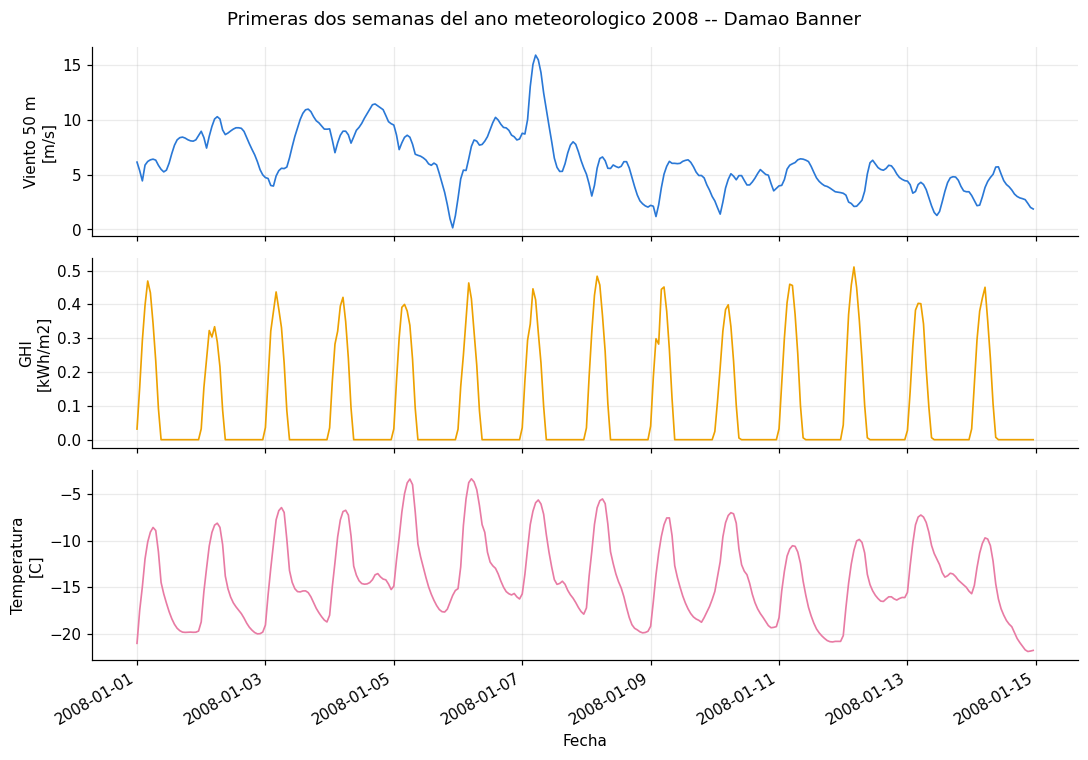
\includegraphics[width=0.92\textwidth]{figures/fig01_recurso_meteorologico.png}
\caption{Recurso meteorológico durante las dos primeras semanas del año 2008 en Damao Banner: velocidad de viento a 50 m, irradiancia global horizontal y temperatura ambiente.}
\label{fig:recurso}
\end{figure}

En el horizonte principal, el recurso reconstruido presenta una velocidad media a 50 m de 7,09 m/s y una irradiancia global horizontal acumulada de 1.658 kWh/m$^2$. Li et al. informa 7,56 m/s y 1.731 kWh/m$^2$; esta diferencia objetiva limita la reproducibilidad del caso antes de aplicar cualquier modelo de conversión.

\section{Decisiones de modelado justificadas por evidencia}
\label{sec:decisiones_modelado}

Tres decisiones del modelo se apartan de la lectura literal del artículo de referencia o resuelven ambigüedades que este deja abiertas. Se documentan aquí de forma explícita porque afectan a los resultados y porque su justificación es empírica y no de conveniencia.

\subsection{Selección de la serie de velocidad de viento}

El artículo declara una altura de buje de 105 m, pero no publica la curva de potencia real, las pérdidas de estela ni otros descuentos necesarios para reconstruir el parque. La serie a 50 m define el escenario principal y la extrapolación a 105 m se evalúa como sensibilidad. No se selecciona una de ellas por su cercanía posterior al LCOE publicado. Por tanto, una diferencia observada no permite concluir qué transformación aplicaron los autores.

\subsection{Corrección de la interpretación de la irradiancia}

Una versión anterior de la implementación interpretaba la irradiancia global horizontal en unidades incompatibles con el modelo térmico de la celda fotovoltaica, lo que producía temperaturas de celda físicamente imposibles y, como consecuencia, una producción fotovoltaica prácticamente nula: el factor de capacidad resultante era del 0,72\,\% frente al 19\,\% publicado. Corregida la interpretación, el factor de capacidad fotovoltaico pasa a 0,1874, con un desvío del $-1{,}34\,\%$.

El episodio se consigna por su valor metodológico. El error no producía excepciones ni resultados manifiestamente absurdos en las magnitudes agregadas: el simulador entregaba costos nivelados plausibles, y solo el contraste sistemático contra indicadores publicados permitió detectarlo. Es un argumento a favor de la verificación cuantitativa frente a la mera inspección de que el código «funciona».

\subsection{Reparto del costo de la batería entre potencia y energía}

El artículo de referencia expresa el costo de la batería exclusivamente por unidad de potencia instalada, imputación coherente con su modelo porque en él la duración está fijada en una hora y potencia y energía resultan numéricamente equivalentes. Al convertir la duración en variable de decisión, esa imputación deja de ser válida: alargar la batería de una a cuatro horas sería gratuito, y la variable carecería de contenido económico.

Se adopta por ello un reparto del costo entre una componente por potencia (30\,\%) y otra por energía (70\,\%), definido de modo que la suma reproduzca el costo original para una duración de una hora. Es una extensión económica introducida por esta tesis, no un parámetro publicado por Li et al.

\begin{table}[H]
\centering
\footnotesize
\caption{Reparto del costo de la batería entre componentes de potencia y de energía}
\label{tab:reparto_bateria}
\renewcommand{\arraystretch}{1.2}
\begin{tabular}{l r r r}
\hline
\textbf{Concepto} & \textbf{Por potencia} & \textbf{Por energía} & \textbf{Suma a 1 h} \\
 & \textbf{[CNY/kW]} & \textbf{[CNY/kWh]} & \textbf{[CNY/kW]} \\
\hline
Inversión inicial & 764{,}70 & 1784{,}30 & 2549{,}00 \\
Reemplazo & 150{,}00 & 350{,}00 & 500{,}00 \\
Operación y mantenimiento anual & 3{,}00 & 7{,}00 & 10{,}00 \\
\hline
\end{tabular}
\end{table}

\section{Modelos de generación y validación del recurso}

La generación eólica se calcula con una curva de potencia cúbica por tramos expresada por unidad de MW y escalada por la capacidad agregada continua $W$. No se redondea el número de turbinas ni se aplica un recorte posterior dependiente de ese redondeo. La generación fotovoltaica aplica un modelo de temperatura de celda basado en la temperatura nominal de operación, con corrección por coeficiente térmico, factor de pérdidas, sobredimensionamiento del generador respecto del inversor y recorte a la potencia nominal de este último.

\begin{figure}[H]
\centering
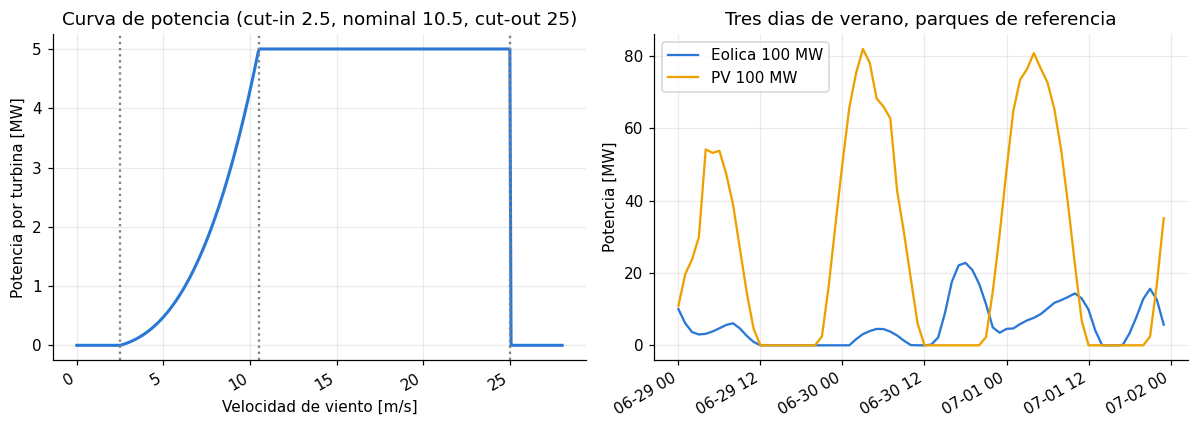
\includegraphics[width=\textwidth]{figures/fig02_curva_potencia_generacion.png}
\caption{Izquierda: curva de potencia de la turbina de 5 MW, con las velocidades de arranque, nominal y de corte. Derecha: perfiles de generación eólica y fotovoltaica de 100 MW durante tres días de verano, donde se aprecia la complementariedad temporal entre ambos recursos.}
\label{fig:generacion}
\end{figure}

La Figura~\ref{fig:generacion} ilustra la complementariedad que justifica la hibridación: la generación fotovoltaica se concentra en las horas centrales del día, mientras que la eólica presenta una distribución más uniforme y con frecuencia máximos nocturnos. Es esta complementariedad la que permite sostener el electrolizador por encima de su carga mínima durante una fracción mayor del año que la alcanzable con cualquiera de los dos recursos por separado.

\section{Modelo económico}

La evaluación económica sigue la estructura de costo presente neto habitual en el dimensionamiento de microrredes \cite{Lambert2006Homer}. Para cada componente se suman la inversión inicial, el valor presente de los reemplazos que correspondan dentro del horizonte de 25 años y el valor presente de los costos anuales de operación y mantenimiento, descontando el valor residual del componente al término del proyecto mediante depreciación lineal sobre la vida útil restante. Con una tasa de descuento real del 4,35\,\% y un horizonte de 25 años, el factor de recuperación de capital resulta de 0,066402.

El electrolizador, con una vida útil de 15 años, incorpora un reemplazo en el año 15; la batería, con una vida útil de 10 años, incorpora reemplazos en los años 10 y 20. El almacenamiento de hidrógeno se dimensiona en 10.000 kg fijos e ingresa al costo presente neto con su inversión y su operación, sin reemplazo ni valor residual por coincidir su vida útil con el horizonte del proyecto.

El costo anualizado se obtiene multiplicando el costo presente neto por el factor de recuperación de capital. El costo nivelado de la energía divide ese costo anualizado por la energía útil anual, definida como la suma de la energía entregada al electrolizador y la vendida a la red. El $\mathrm{LCOH}_{\mathrm{tesis}}$ divide el mismo costo anualizado por la producción anual de hidrógeno; es un indicador secundario con la asignación de costos propia ya declarada.

\section{Simulación horaria y despacho}

Cada configuración candidata se evalúa mediante una simulación secuencial de las 8.760 horas del horizonte principal. El estado de carga de la batería en cada hora depende del estado precedente; por ello el despacho se calcula cronológicamente. La sensibilidad de 8.784 horas ejecuta el mismo algoritmo sin retirar el 29 de febrero.

El despacho horario aplica una prioridad fija sobre la energía renovable disponible: primero alimentar el electrolizador, después cargar la batería con el excedente, a continuación exportar a la red y, finalmente, verter el remanente que exceda la capacidad de conexión. El modelo no permite compras de electricidad a la red; $P_{grid,t}$ representa solo exportación no negativa. La carga auxiliar de planta se fija en cero porque su magnitud no está publicada, mientras que las eficiencias del rectificador y del convertidor bidireccional se aplican explícitamente. Las dos políticas de gestión de la carga mínima del electrolizador, que constituyen una de las diferencias entre las dos instancias de optimización, se detallan en el capítulo de diseño experimental.

Concluida la simulación, se calculan los agregados anuales, se verifica la restricción sobre la fracción de energía vendida a la red y se evalúan los indicadores económicos. Cuando una configuración incumple una restricción verificable antes de simular, la función de evaluación retorna un resultado infactible acompañado del motivo textual del rechazo, lo que facilita la depuración y permite auditar por qué una región del dominio quedó excluida.

\section{Parámetros del escenario}

Las Tablas~\ref{tab:parametros_configuracion_replica}--\ref{tab:parametros_costos_conversion_replica} recogen los parámetros empleados. Se usan los valores publicados por Li et al. cuando están disponibles \cite{Li2024WPEB}; las coordenadas aproximadas, la serie meteorológica, la carga auxiliar nula, las reglas de despacho y el reparto del costo de batería se identifican expresamente como supuestos de reconstrucción o extensiones de esta tesis.

\begingroup
\setlength{\tabcolsep}{3pt}
\renewcommand{\arraystretch}{1.15}
\footnotesize

\begin{table}[H]
\centering
\caption{Emplazamiento y horizonte temporal}
\label{tab:parametros_configuracion_replica}
\begin{tabular}{p{4.2cm} p{3.0cm} p{8.1cm}}
\hline
\textbf{Parámetro} & \textbf{Valor} & \textbf{Descripción} \\
\hline
\textbf{Latitud} & 41,70 & Latitud aproximada de Damao Banner, Baotou, Mongolia Interior. \\
\textbf{Longitud} & 110,43 & Longitud aproximada del mismo emplazamiento. \\
\textbf{Zona horaria} & UTC+8 & Zona horaria local, relevante para la complementariedad viento-solar. \\
\textbf{Año de análisis} & 2008 & Año meteorológico empleado, por consistencia con el artículo de referencia. \\
\textbf{Horizonte principal} & 8.760 h & Reproducción del horizonte declarado por Li et al.; se retira el 29 de febrero. \\
\textbf{Sensibilidad temporal} & 8.784 h & Año bisiesto completo con resolución horaria. \\
\textbf{Fuente de datos} & NASA POWER & Serie horaria de viento, irradiancia y temperatura. \\
\hline
\end{tabular}
\end{table}

\begin{table}[H]
\centering
\caption{Restricciones del problema y resolución del barrido de la instancia base}
\label{tab:parametros_busqueda_replica}
\begin{tabular}{p{4.2cm} p{3.0cm} p{8.1cm}}
\hline
\textbf{Parámetro} & \textbf{Valor} & \textbf{Descripción} \\
\hline
\textbf{Capacidad renovable total} & 200,0 MW & Capacidad renovable fija del sistema, $W+P=200$ MW. \\
\textbf{AGSR máximo} & 0,20 & Límite de la fracción anual de energía renovable vendida a la red. \\
\textbf{Razón máxima del electrolizador} & 0,50 & Límite superior $E \leq 0{,}5(W+P)$, es decir 100 MW. \\
\textbf{Paso de capacidad eólica} & 10,0 MW & Discretización de la capacidad eólica en el barrido exhaustivo. \\
\textbf{Paso del electrolizador} & 5,0 MW & Discretización de la capacidad de electrólisis en el barrido. \\
\textbf{Razón batería/electrolizador} & 0,30 & Regla de dimensionamiento derivado de la batería en la instancia base. \\
\textbf{Redondeo de potencia de batería} & 2,5 MW & Paso de redondeo aplicado a la potencia derivada. \\
\hline
\end{tabular}
\end{table}

\begin{table}[H]
\centering
\caption{Supuestos técnicos y energéticos}
\label{tab:parametros_tecnicos_replica}
\begin{tabular}{p{4.2cm} p{3.0cm} p{8.1cm}}
\hline
\textbf{Parámetro} & \textbf{Valor} & \textbf{Descripción} \\
\hline
\textbf{HHV del hidrógeno} & 39,4 kWh/kg & Poder calorífico superior empleado para el balance de masa. \\
\textbf{Eficiencia del electrolizador} & 0,75 & Eficiencia energética; implica 52,53 kWh por kg de H$_2$. \\
\textbf{Carga mínima del electrolizador} & 0,30 & Fracción mínima de carga para operar. \\
\textbf{Módulo de electrólisis} & 5,0 MW & Tamaño unitario en la instancia mixta (10 a 20 módulos). \\
\textbf{Almacenamiento de H$_2$} & 10.000 kg & Capacidad fija del tanque; no es variable de decisión. \\
\textbf{Vida del proyecto} & 25 años & Horizonte económico. \\
\textbf{Tasa de descuento real} & 0,0435 & Tasa empleada en el descuento de flujos. \\
\textbf{Potencia nominal de turbina} & 5,0 MW & Potencia por unidad del parque eólico. \\
\textbf{Velocidades de la turbina} & 2,5 / 10,5 / 25,0 m/s & Arranque, nominal y corte. \\
\textbf{Serie de viento empleada} & \texttt{ws50m} & Velocidad medida a 50 m (véase Sección~\ref{sec:decisiones_modelado}). \\
\textbf{Relación DC/AC fotovoltaica} & 1,2 & Sobredimensionamiento del generador respecto del inversor. \\
\textbf{Coeficiente térmico FV} & $-0{,}5$ \%/$^\circ$C & Coeficiente de temperatura de potencia. \\
\textbf{NOCT} & 47,0 $^\circ$C & Temperatura nominal de operación de celda. \\
\textbf{Factor de reducción FV} & 0,90 & Pérdidas del sistema fotovoltaico. \\
\textbf{Eficiencias de conversión} & 0,95 & Inversor, rectificador y convertidor bidireccional. \\
\textbf{Eficiencia de la batería} & 0,90 & Eficiencia de ciclo completo. \\
\hline
\end{tabular}
\end{table}

\begin{table}[H]
\centering
\caption{Costos de los componentes de generación renovable}
\label{tab:parametros_costos_renovables_replica}
\begin{tabular}{p{4.2cm} p{3.0cm} p{8.1cm}}
\hline
\textbf{Parámetro} & \textbf{Valor} & \textbf{Descripción} \\
\hline
\textbf{Inversión eólica} & 5917,0 CNY/kW & Costo de inversión inicial del parque eólico. \\
\textbf{Reemplazo eólico} & 0,0 CNY/kW & Sin reemplazo dentro del horizonte de 25 años. \\
\textbf{O\&M eólico} & 40,2 CNY/kW-año & Costo anual de operación y mantenimiento. \\
\textbf{Vida útil eólica} & 25 años & Coincide con el horizonte del proyecto. \\
\textbf{Inversión fotovoltaica} & 4633,0 CNY/kW & Costo de inversión inicial del campo fotovoltaico. \\
\textbf{Reemplazo fotovoltaico} & 0,0 CNY/kW & Sin reemplazo dentro del horizonte. \\
\textbf{O\&M fotovoltaico} & 17,6 CNY/kW-año & Costo anual de operación y mantenimiento. \\
\textbf{Vida útil fotovoltaica} & 25 años & Coincide con el horizonte del proyecto. \\
\hline
\end{tabular}
\end{table}

\begin{table}[H]
\centering
\caption{Costos de conversión, almacenamiento electroquímico y almacenamiento de hidrógeno}
\label{tab:parametros_costos_conversion_replica}
\begin{tabular}{p{4.2cm} p{3.0cm} p{8.1cm}}
\hline
\textbf{Parámetro} & \textbf{Valor} & \textbf{Descripción} \\
\hline
\textbf{Inversión electrolizador} & 6964,0 CNY/kW & Costo de inversión inicial. \\
\textbf{Reemplazo electrolizador} & 5969,14 CNY/kW & Reemplazo aplicado en el año 15. \\
\textbf{O\&M electrolizador} & 208,92 CNY/kW-año & Costo anual de operación y mantenimiento. \\
\textbf{Vida útil electrolizador} & 15 años & Determina un reemplazo dentro del horizonte. \\
\textbf{Inversión batería} & 764,70 / 1784,30 & Por kW y por kWh respectivamente (Tabla~\ref{tab:reparto_bateria}). \\
\textbf{Reemplazo batería} & 150,00 / 350,00 & Por kW y por kWh; reemplazos en los años 10 y 20. \\
\textbf{O\&M batería} & 3,00 / 7,00 & Por kW-año y por kWh-año respectivamente. \\
\textbf{Vida útil batería} & 10 años & Determina dos reemplazos dentro del horizonte. \\
\textbf{Inversión almacenamiento H$_2$} & 6611,77 CNY/kg & Tanque de 10.000 kg; ingresa al costo presente neto. \\
\textbf{O\&M almacenamiento H$_2$} & 141,68 CNY/kg-año & Costo anual de operación y mantenimiento. \\
\textbf{Vida almacenamiento H$_2$} & 25 años & Sin reemplazo ni valor residual. \\
\hline
\end{tabular}
\end{table}

\endgroup

\chapter{Diseño experimental}

Este capítulo define las instancias, el óptimo exacto que sirve de referencia, la configuración de los nueve algoritmos y el protocolo de comparación. El simulador horario es común a todos los métodos y a todas las instancias; lo único que cambia entre competidores es el operador de búsqueda. Esta separación evita atribuir al algoritmo diferencias causadas por modelos energéticos distintos.

\section{Instancias de optimización}
\label{sec:instancias_experimento}

El Capítulo 2 formuló el problema sobre el dominio mixto de la ecuación~\eqref{eq:dominio} y definió una instancia como la tupla $(C_{tot},\mathrm{AGSR}_{max},u,n_{min},n_{max},\Delta_B,B_{max},\{h_k\})$. Las cuatro instancias de la Tabla~\ref{tab:instancias_auto} derivan de la de referencia cambiando un aspecto cada vez, de modo que cualquier diferencia de comportamiento entre instancias tiene una causa declarada:

\begin{itemize}
    \item \textbf{I1, instancia mixta de referencia.} $C_{tot}=200$ MW, $\mathrm{AGSR}_{max}=0{,}20$, módulos de electrólisis de 5 MW ($n_E\in\{10,\ldots,20\}$), batería de 0 a 50 MW en pasos de 5 MW y duraciones de 1, 2 y 4 h: \InstCatalogsA{} catálogos discretos por valor de $W$.
    \item \textbf{I2, región factible estrecha.} Igual que I1 con $\mathrm{AGSR}_{max}=0{,}10$. Sólo cambia la restricción C5, que es la activa en el óptimo; la fracción factible del dominio cae de \BFAFeasiblePct\,\% a \BFBFeasiblePct\,\%.
    \item \textbf{I3, catálogos finos.} Igual que I1 con módulos de 2,5 MW ($n_E\in\{20,\ldots,40\}$), pasos de batería de 2,5 MW y duraciones de 1, 2, 4 y 8 h: \InstCatalogsC{} catálogos sobre la misma región física, lo que multiplica por cinco las combinaciones discretas que un método debe discriminar.
    \item \textbf{I4, escala.} $C_{tot}=300$ MW con electrolizador de hasta 150 MW ($n_E\in\{10,\ldots,30\}$) y el catálogo de batería de I1, para aislar el efecto de escala sobre $W$ y $E$: \InstCatalogsD{} catálogos.
\end{itemize}

La \textbf{instancia base} de Li et al. \cite{Li2024WPEB}, en la que $W$ y $E$ son los grados de libertad efectivos, $P=200-W$ y la batería se deriva como el 30\,\% del electrolizador redondeado a módulos de 2,5 MW con política de despacho \texttt{TOP\_UP}, se conserva únicamente como caso de validación y para los barridos de sensibilidad. Sus 420 puntos se enumeran y su mejor valor sólo puede llamarse óptimo \emph{sobre esa malla}. Los algoritmos no se comparan sobre ella: la política de despacho (\texttt{THRESHOLD}) y el espacio de batería de las instancias mixtas son distintos, y comparar sus valores con los de la instancia base no mediría una mejora producida por las metaheurísticas.

\section{Espacio de decisión}

Los optimizadores manipulan $\mathbf{x}\in\mathbb{R}^4$. Antes de simular, el vector se recorta a sus límites y se decodifica según la Tabla~\ref{tab:espacio_decision}; los límites y pasos dependen de la instancia.

\begin{table}[H]
\centering
\footnotesize
\caption{Variables de decisión y su decodificación en las instancias mixtas}
\label{tab:espacio_decision}
\renewcommand{\arraystretch}{1.2}
\begin{tabular}{c p{3.7cm} c c p{5.6cm}}
\hline
\textbf{Índice} & \textbf{Variable} & \textbf{Lím. inf.} & \textbf{Lím. sup.} & \textbf{Decodificación} \\
\hline
$x_0$ & Capacidad eólica $W$ [MW] & 0 & $C_{tot}$ & Continua; $P=C_{tot}-W$ \\
$x_1$ & Módulos de electrólisis $n_E$ & $n_{min}$ & $n_{max}$ & Entero más cercano; $E=u\,n_E$ MW \\
$x_2$ & Potencia de batería $B^P$ [MW] & 0 & $B_{max}$ & Múltiplo de $\Delta_B$ más cercano \\
$x_3$ & Índice de duración $k$ & 0 & $K-1$ & Entero más cercano; $h_B=h_k$ si $B^P>0$ \\
\hline
\end{tabular}
\end{table}

Cuando $B^P=0$, la duración se fija en cero: las $K$ etiquetas de duración describirían el mismo diseño físico y no deben contarse como alternativas distintas. Por ello el número de catálogos efectivos por valor de $W$ es $(n_{max}-n_{min}+1)\,(1+K\,B_{max}/\Delta_B)$, que da \InstCatalogsA{}, \InstCatalogsB{}, \InstCatalogsC{} e \InstCatalogsD{} para I1 a I4. Todo vector tiene un \textbf{representante canónico}, obtenido al decodificar y volver a codificar, que la búsqueda local de los híbridos usa como punto de partida.

La potencia eólica se modela como capacidad agregada continua. Si $p_{wt,t}^{pu}$ es la curva de potencia de una turbina normalizada por su potencia nominal, entonces
\begin{equation}
P_{wt,t}=W\,p_{wt,t}^{pu}.
\end{equation}
No se redondea $W$ a un número entero de turbinas. Esta idealización debe interpretarse como planificación de capacidad agregada, no como selección final de equipos.

\section{Función objetivo e indicadores}

El problema es monoobjetivo, ecuación~\eqref{eq:problema}: se minimiza el LCOE, cociente entre el costo anualizado y la energía útil anual (entregada al electrolizador más vendida a la red), con el factor 1000 que convierte MWh en kWh. El NPC y el LCOH se calculan como indicadores secundarios y no intervienen en el orden de aptitud. En particular,
\begin{equation}
\mathrm{LCOH}_{tesis}=\frac{C_{ann}}{M_{H_2}},
\end{equation}
asigna el costo anualizado total a la producción de hidrógeno, sin acreditar la electricidad exportada. Por esta diferencia de asignación y por la información incompleta del artículo antecedente \cite{Li2023TechnoEconomic}, se denomina ``LCOH según esta tesis'' y no se trata como una reproducción directa del LCOH publicado.

\section{Cinco grupos de restricciones}

\begin{table}[H]
\centering
\scriptsize
\caption{Restricciones, procedencia y mecanismo de cumplimiento}
\label{tab:restricciones}
\renewcommand{\arraystretch}{1.22}
\begin{tabular}{@{}p{0.6cm} p{4.3cm} p{2.2cm} p{2.2cm} p{3.0cm}@{}}
\hline
\textbf{ID} & \textbf{Formulación} & \textbf{Unidad} & \textbf{Procedencia} & \textbf{Tratamiento} \\
\hline
C1 & $P_{ren,t}+P_{desc,t}=P_{E,t}+P_{carga,t}+P_{grid,t}+P_{vert,t}$ & MW, cada hora & Balance de Li et al. y simulador & Ecuación de estado; residuo auditado \\
C2 & $W+P=C_{tot}$, $W\geq0$, $P\geq0$ & MW & Li et al. & Parametrización $P=C_{tot}-W$ y recorte \\
C3 & $0<E\leq0{,}5\,C_{tot}$ & MW & Li et al. & Límites del catálogo y decodificación \\
C4 & $0\leq SOC_t\leq B^E$; $P_{carga,t}\leq B^P$; $P_{desc,t}\leq B^P$; carga del electrolizador nula o superior al mínimo & MWh y MW & Modelo operacional de esta tesis & Despacho horario y verificación posterior \\
C5 & $\mathrm{AGSR}=E_{grid}/E_{ren}\leq\mathrm{AGSR}_{max}$ & fracción anual & Li et al.; $\mathrm{AGSR}_{max}$ según la instancia & Verificación tras la simulación \\
\hline
\end{tabular}
\end{table}

La factibilidad se compara mediante las reglas de Deb \cite{Deb2000Constraint}. Toda solución factible domina a una infactible; entre dos infactibles se prefiere la menor suma de violaciones normalizadas, y entre dos factibles se minimiza LCOE. Esto elimina el peso arbitrario $10^6$ empleado en la versión preliminar. El residuo máximo de C1 y las violaciones de C2--C5 se almacenan por separado.

\section{Óptimo exacto por fuerza bruta}
\label{sec:fuerza_bruta}

Para cada instancia se enumeran \textbf{todos} los catálogos discretos efectivos sobre \textbf{todos} los valores $W\in\{0;\,0{,}01;\,\ldots;\,C_{tot}\}$ MW, sin muestreo ni poda: entre \BFADesigns{} (I1) y \BFCDesigns{} (I3) diseños anuales por instancia, \BruteForceDesignsTotal{} en total. El mejor diseño factible de esa enumeración es el \textbf{óptimo exacto del dominio discretizado}, único referente de las brechas y tasas de éxito.

Ese volumen es abordable porque el despacho \texttt{THRESHOLD} se reescribe de forma vectorizada: el bucle horario sigue siendo secuencial por el estado de carga, pero cada hora se resuelve simultáneamente para todos los diseños de un bloque de 150 valores de $W$, y el costo presente neto, lineal en cada capacidad, se obtiene del aporte unitario por kW y por kWh. Cada bloque se reduce al vuelo al mejor $W$ por catálogo y a la envolvente inferior por $W$, de modo que nunca se retienen matrices completas. Tres verificaciones preceden a la aceptación de un óptimo: la réplica vectorizada se contrasta contra el simulador oficial en 200 celdas aleatorias de la malla, con diferencia relativa máxima de LCOE de \MaxControlRelDiff{}; los diez mejores catálogos se recalculan con el simulador oficial, que verifica los cinco grupos de restricciones; y se evalúa el diseño un paso de malla más allá del óptimo, dentro del mismo catálogo, para comprobar que la restricción C5 es la que detiene la mejora. El resultado reducido de cada instancia se guarda en disco con una huella del escenario, de los datos y del paso, de modo que repetir el cuaderno tras modificar un algoritmo no vuelve a pagar las horas de enumeración.

Como $W$ es continuo en los optimizadores y discretizado a 0,01 MW en la enumeración, un optimizador puede terminar marginalmente por debajo del óptimo exacto; la brecha se informa con signo y se tolera hasta $-0{,}01$\,\%.

\section{Selección y configuración de los algoritmos}

La selección busca diversidad de mecanismos, no representatividad exhaustiva de toda la literatura. Entre los clásicos, PSO y GA actúan como referencias consolidadas; GWO combina tres líderes; WOA alterna cerco, exploración aleatoria y espiral; SHO incorpora una agrupación dinámica; y la búsqueda aleatoria establece cuánto puede lograrse sin aprendizaje. WOA cuenta además con aplicaciones publicadas en sistemas renovables con hidrógeno \cite{Sun2022WOA}, mientras que SHO dispone de estudios específicos sobre tamaño de población y terminación \cite{Vega2022SHO}; estas referencias motivan su inclusión, no garantizan su desempeño en estas instancias. Los tres híbridos se construyen sobre esos clásicos sin modificarlos, de modo que cada uno tiene un padre identificable con el que compararse. La Tabla~\ref{tab:hiperparametros_auto} se genera desde la configuración efectivamente ejecutada.

\TablaHiperparametrosAuto

No se ajustaron hiperparámetros después de observar los resultados, ni en los clásicos ni en los híbridos. La regla de vecindad usada para operacionalizar \texttt{count\_nos} en SHO se declara porque el artículo original no la define inequívocamente: se normalizan las distancias a la mejor hiena, se sortea un radio en $[0{,}5,1]$ y se incluyen las soluciones dentro de él, siempre con al menos la mejor. Por ello la implementación sigue las fases y ecuaciones publicadas, pero no se presenta esa regla particular como información proporcionada por los autores \cite{Dhiman2017SHO}.

\subsection{Infraestructura de hibridación}

Los seis clásicos consumen exactamente $\text{población}\times\text{iteraciones}$ solicitudes por construcción y registran su historial al cierre de cada iteración. Un híbrido con búsqueda local no tiene un número fijo de generaciones, así que la clase base de los optimizadores incorpora un \textbf{contrato de presupuesto}: toda solicitud de los híbridos pasa por un método que rechaza cualquier evaluación por encima de las \RequestsPerRun{} de la corrida y que registra un punto de control del historial cada \Population{} solicitudes. Así el historial de un híbrido tiene exactamente \Iterations{} filas y es comparable, a igual número de solicitudes, con el de los clásicos; la figura de convergencia usa por ello las solicitudes acumuladas como abscisa. Al cierre de cada corrida se verifica que el número de solicitudes coincide con el presupuesto.

La \textbf{búsqueda local} es común a GA+LS y SHO+LS. Parte del representante canónico de un diseño ya evaluado y recorre, en orden fijo, los vecinos $W\pm\delta_W$, $n_E\pm1$, $B^P\pm\Delta_B$ y $k\pm1$; cada coordenada recuerda la dirección del último éxito y la prueba primero. Acepta el \textbf{primer vecino que mejora} según las reglas de Deb y reanuda desde él (mejora lamarckiana: el vector mejorado reemplaza al individuo o presa que la originó). El paso continuo $\delta_W$ empieza en el 1\,\% del rango de $W$ y se contrae a la mitad cada vez que el vecindario completo falla, hasta un mínimo igual al paso de la fuerza bruta, 0,01 MW, de modo que la búsqueda local nunca resuelve $W$ más fino que el óptimo certificado. Los vecinos fuera de límites, los que decodifican al mismo diseño (por ejemplo $k\pm1$ con $B^P=0$) y los que ya están en el caché de la corrida se omiten sin solicitar nada; si todo el vecindario está agotado y $\delta_W$ es mínimo, la búsqueda devuelve sin gastar y el presupuesto sobrante lo consume el bucle poblacional. Cada llamada dispone de a lo sumo 4 solicitudes y se registran las solicitudes y mejoras que efectivamente consumió.

\subsection{Los tres híbridos}

\begin{itemize}
    \item \textbf{GA+LS (algoritmo genético memético).} Conserva íntegro el GA: mismo torneo, mismo cruce BLX-$\alpha$, misma mutación gaussiana y mismo elitismo. En cada generación, tras evaluar los \Population{} individuos, el mejor recibe la búsqueda local y la generación siguiente se produce con los operadores del GA. Cada generación cuesta hasta 24 solicitudes, de modo que el presupuesto alcanza para 25 en lugar de las 30 del GA puro; la hipótesis sometida a prueba es que la intensificación compensa las generaciones de exploración perdidas.
    \item \textbf{PSO+GA (enjambre con operadores genéticos).} Conserva íntegro el bucle del PSO, incluida la actualización de velocidad con constricción. Al final de cada iteración, las 5 partículas de peor mérito actual se reemplazan por hijos producidos con los operadores del GA: padres por torneo ($k=3$) sobre las mejores posiciones personales del enjambre, cruce BLX-$\alpha$ con $p_c=0{,}9$ y mutación gaussiana. El hijo arranca con velocidad nula y sin memoria personal. No hay búsqueda local, así que mantiene las 30 iteraciones de 20 solicitudes.
    \item \textbf{SHO+LS (SHO con búsqueda local).} Conserva íntegro el SHO, incluida la regla declarada para \texttt{count\_nos}. Tras evaluar las 20 hienas, la presa recibe la búsqueda local y la presa mejorada guía el cerco. El coeficiente $h$ decae de $h_{max}$ a 0 sobre las 25 generaciones que caben en el presupuesto. SHO se eligió por ser el enjambre clásico de mejor mediana en la comparativa preliminar sobre I1; la elección se fijó antes de correr el experimento de cuatro instancias.
\end{itemize}

Los tres son híbridos integrativos de bajo nivel (LTH) en la taxonomía de Talbi \cite{Talbi2002Taxonomy}; PSO+GA es además heterogéneo. GWO+LS sería la alternativa inmediata con la misma infraestructura; se deja fuera para mantener un híbrido por familia.

\section{Presupuesto, referencia y reproducibilidad}

Cada método recibe \RequestsPerRun{} solicitudes de función objetivo por ejecución, incluida la población inicial: \Population{} individuos durante \Iterations{} iteraciones, o su equivalente en solicitudes para los híbridos. Las propuestas repetidas cuentan contra el presupuesto; se informan además diseños únicos, duplicados, solicitudes de la búsqueda local, llamadas reales al simulador y tiempo. Se realizan \Replicates{} ejecuciones independientes por método y por instancia: \RequestsPerInstance{} evaluaciones de diseños anuales por instancia y \TotalDesignRequests{} en total, en \TotalRuns{} corridas. Los identificadores 42--71 generan flujos separados mediante la pareja algoritmo--réplica, independientes de la instancia; no constituyen bloques pareados. Como los clásicos no se modifican y el flujo aleatorio no depende de la instancia, la corrida de I1 reproduce bit a bit la comparativa previa de seis algoritmos, lo que se verificó antes de ejecutar el experimento.

Las implementaciones se someten previamente a pruebas deterministas: una actualización de GWO, SHO, WOA y de la inyección genética de PSO+GA contrastada contra sus ecuaciones con semilla fija; la búsqueda local sobre un bol cuadrático con una coordenada discreta, donde debe alcanzar el óptimo a la resolución mínima y terminar sin agotar el presupuesto; la ausencia de solicitudes duplicadas de la búsqueda local sobre el objetivo real; el presupuesto e historial exactos de los tres híbridos; y pruebas de límites, presupuesto y dirección de minimización de clásicos e híbridos sobre Sphere y Rastrigin. El simulador exige además 8.760 registros en el caso principal, 8.784 en la sensibilidad y un residuo de balance inferior a $10^{-8}$ MW.

\section{Análisis comparativo}

Dentro de cada instancia, el análisis descriptivo usa mediana, rango intercuartílico, mejor y peor valor, brecha respecto del óptimo exacto y probabilidades empíricas de quedar a menos de 0,1\,\%, 0,5\,\% y 1\,\% de él. La desviación típica se conserva como descriptor, pero no se interpreta aisladamente como consistencia.

Las \Replicates{} ejecuciones por algoritmo e instancia se tratan como muestras independientes. La inferencia se hace dentro de cada instancia con Kruskal--Wallis como contraste global y Mann--Whitney bilateral por pares, con $A_{12}$ de Vargha--Delaney e intervalos bootstrap al 95\,\%. Con nueve algoritmos hay 36 pares por instancia y corregir por Holm sobre los 36 sacrifica potencia en contrastes que no interesan; por eso el análisis principal usa una \textbf{familia planificada de 12 contrastes por instancia}, fijada antes de ejecutar el experimento: cada una de las ocho metaheurísticas frente a RANDOM y cada híbrido frente a su padre o padres (GA+LS vs GA, PSO+GA vs PSO, PSO+GA vs GA, SHO+LS vs SHO), con Holm dentro de la familia. La matriz completa se calcula igualmente, con Holm sobre los 36 pares, y se relega al anexo.

La lectura transversal resume las cuatro instancias mediante el rango por mediana de cada algoritmo en cada instancia y su rango medio. Es descriptiva: cuatro instancias no justifican un contraste de Friedman, y las instancias no se comparan entre sí porque difieren en región factible y en escala. Ninguna comparación establece superioridad general entre algoritmos fuera de estas instancias, presupuesto e hiperparámetros.

\section{Protocolo de reproducción de Li et al.}

El artículo declara un año de 8.760 horas, aunque 2008 fue bisiesto \cite{Li2024WPEB}. La reproducción principal elimina exactamente las 24 marcas del 29 de febrero; la serie íntegra de 8.784 horas se evalúa por separado. Se mantienen las coordenadas aproximadas $(41{,}70;110{,}43)$ sin calibrarlas contra las salidas publicadas.

Para W190--P10--E95--B30, W120--P80--E80--B25 y W60--P140--E85--B27,5 se reportan recurso, generación, hidrógeno, NPC, LCOE, LCOH según esta tesis y AGSR. Cada magnitud comparable incluye diferencia absoluta y error relativo; las etiquetas ``estrecha'' ($\leq5$\,\%), ``parcial'' ($5$--$25$\,\%) y ``no reproducida'' ($>25$\,\%) son descripciones, no criterios de aceptación pre-registrados.

La serie de viento a 50 m define el caso principal y la extrapolada a 105 m constituye una sensibilidad. Las coordenadas, la versión del recurso, el año bisiesto, las pérdidas, la carga auxiliar y el despacho se reconocen como fuentes conjuntas de incertidumbre. Ninguna discrepancia se atribuye de manera exclusiva al artículo. Asimismo, cualquier exceso de AGSR se redacta como resultado condicionado a los datos y al despacho reconstruidos.

\chapter{Resultados}

Este capítulo presenta los resultados en seis bloques: reproducción de Li et al. \cite{Li2024WPEB}, óptimo exacto de cada instancia, comparación de los nueve algoritmos dentro de cada instancia, lectura transversal, híbridos frente a sus padres y sensibilidad. Todas las cifras producidas por esta investigación se generan desde los archivos CSV exportados por el cuaderno; los dos valores transcritos directamente de la fuente se identifican como tales.

\section{Reproducción del modelo publicado}

\subsection{Recurso meteorológico y casos de contraste}

La reproducción principal utiliza \HoursMain{} horas. Se retiraron exactamente las 24 observaciones del 29 de febrero de 2008 de la serie original y se mantuvieron las coordenadas aproximadas $(41{,}70;110{,}43)$ sin ajustarlas para acercar las salidas al artículo. La serie local procede de NASA POWER; el archivo de procedencia registra columnas, coordenadas y resolución, pero declara la versión de API como no registrada en el artefacto original. Esta limitación no se oculta ni se completa retrospectivamente con una versión actual.

\TablaValidacionAuto

Los errores no respaldan una declaración de reproducción exacta. La mayoría de los indicadores presenta proximidad estrecha o parcial, pero esa concordancia depende de una reconstrucción que no dispone de la coordenada exacta, de la serie meteorológica de los autores ni de todos sus detalles de despacho. Por ello el resultado se califica como \textbf{reproducción parcial bajo supuestos explícitos}.

\TablaCasosAuto

La Tabla~\ref{tab:casos_auto} separa magnitudes energéticas y económicas del juicio de factibilidad. Cuando AGSR supera 0,20, la conclusión correcta es que la configuración excede el límite \emph{bajo los datos y el despacho reconstruidos}; no demuestra que la solución publicada sea intrínsecamente infactible.

El LCOH no admite una validación directa. Li et al. informa para W190 dos cifras incompatibles, 10,6248 CNY/kg en la Sección 3.2 y 14,1574 CNY/kg en las conclusiones. Además, la asignación de costos no puede reconstruirse inequívocamente a partir del artículo de 2024 y su antecedente de 2023 \cite{Li2023TechnoEconomic}. En consecuencia, el cuaderno reporta $\mathrm{LCOH}_{\mathrm{tesis}}$ como indicador secundario y no lo usa para afirmar concordancia con la fuente.

\begin{table}[H]
\centering
\footnotesize
\caption{Valores de LCOH publicados por Li et al. para el caso W190}
\label{tab:lcoh_inconsistente}
\begin{tabular}{l r}
\hline
\textbf{Ubicación en la fuente} & \textbf{LCOH [CNY/kg]} \\
\hline
Sección 3.2 & 10,6248 \\
Conclusiones & 14,1574 \\
\hline
\end{tabular}
\end{table}

\subsection{Efecto del año bisiesto y de la altura del viento}

\TablaHorizonteAuto

La serie completa de \HoursSensitivity{} horas se interpreta exclusivamente como sensibilidad. Para la mejor corrida de I1, incluir el 29 de febrero modifica el LCOE en \BestHorizonDeltaPct\,\%. Esta magnitud permite acotar el efecto temporal sin presentar 8.784 horas como el horizonte declarado por Li et al.

\TablaAlturaVientoAuto

La extrapolación desde 50 m hasta 105 m altera simultáneamente generación, AGSR y LCOE. Se muestran ambas alternativas y se conserva la serie bruta a 50 m como caso principal; no se selecciona retrospectivamente la que reproduce mejor un indicador económico.

\subsection{Evolución de la reconstrucción}

\TablaEvolucionAuto

La discrepancia preliminar de hasta 95,16\,\% se conserva como antecedente. La reducción posterior del error coincide con cambios documentados en horizonte, escalamiento de la capacidad eólica y auditoría de supuestos. Esta trazabilidad evita presentar la versión final como si hubiera sido obtenida sin iteraciones y, al mismo tiempo, impide atribuir inequívocamente la discrepancia inicial a una sola causa.

\section{Las instancias y su óptimo exacto}

\subsection{Malla base de Li et al.}

La malla base contiene \BaseEvaluated{} puntos, de los cuales \BaseFeasible{} (\BaseFeasiblePct\,\%) satisfacen las restricciones bajo la reconstrucción. El mejor punto de esa malla tiene $W=\BaseBestWind$ MW, $E=\BaseBestElectrolyzer$ MW y LCOE de \BaseBestLCOE{} CNY/kWh. Esta es una afirmación de optimalidad limitada a la malla base finita.

\begin{figure}[H]
\centering
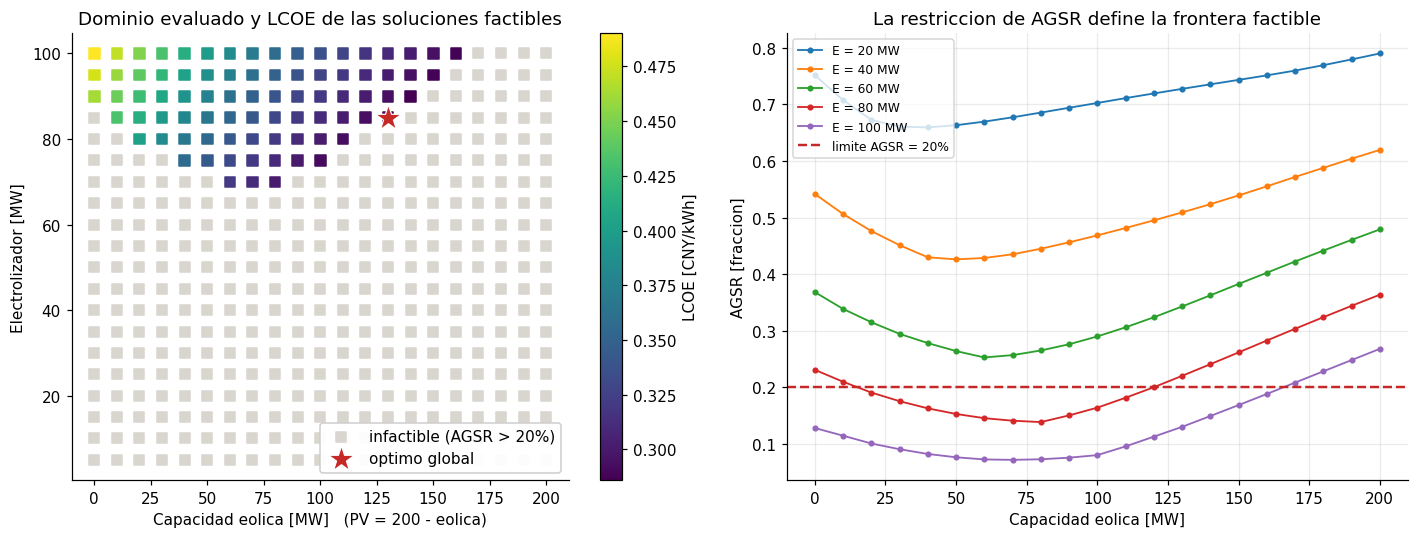
\includegraphics[width=0.95\textwidth]{figures/fig03_dominio_instancia_base.png}
\caption{LCOE y factibilidad de los 420 puntos de la instancia base de Li et al. La estrella identifica el mejor punto de esta malla, no un óptimo del dominio mixto.}
\label{fig:dominio_base}
\end{figure}

\subsection{Óptimos por fuerza bruta}

La Tabla~\ref{tab:fuerza_bruta_auto} resume la enumeración completa de cada instancia: diseños evaluados, fracción factible, óptimo exacto y tiempo de cómputo. En total se evaluaron \BruteForceDesignsTotal{} diseños anuales en \BruteForceElapsedHours{} horas de cómputo, con una diferencia relativa máxima de \MaxControlRelDiff{} entre la réplica vectorizada y el simulador oficial en las celdas de control.

\TablaFuerzaBrutaAuto

Los óptimos exactos son LCOE $=\BFALCOE$ CNY/kWh en I1 ($W=\BFAWind$ MW, $E=\BFAElectrolyzer$ MW, batería de \BFABattery{} MW durante \BFADuration{} h), \BFBLCOE{} en I2 ($W=\BFBWind$, $E=\BFBElectrolyzer$, \BFBBattery{} MW $\times$ \BFBDuration{} h), \BFCLCOE{} en I3 ($W=\BFCWind$, $E=\BFCElectrolyzer$, \BFCBattery{} MW $\times$ \BFCDuration{} h) y \BFDLCOE{} en I4 ($W=\BFDWind$, $E=\BFDElectrolyzer$, \BFDBattery{} MW $\times$ \BFDDuration{} h). En las cuatro instancias el óptimo se sitúa sobre el borde de la restricción C5, con AGSR de \BFAAGSR, \BFBAGSR, \BFCAGSR{} y \BFDAGSR{} respectivamente, y el diseño un paso de malla más allá en $W$ viola esa restricción: la fracción vendida a la red es lo que detiene la mejora, no el costo. Reducir el límite a 0,10 (I2) encarece el óptimo en más de un diez por ciento y desplaza el diseño hacia menos eólica y más electrólisis; refinar los catálogos (I3) permite un óptimo marginalmente mejor que el de I1 al disponer de combinaciones intermedias; y la escala de 300 MW (I4) reduce el LCOE por el reparto del almacenamiento de hidrógeno fijo sobre más energía.

\begin{figure}[H]
\centering
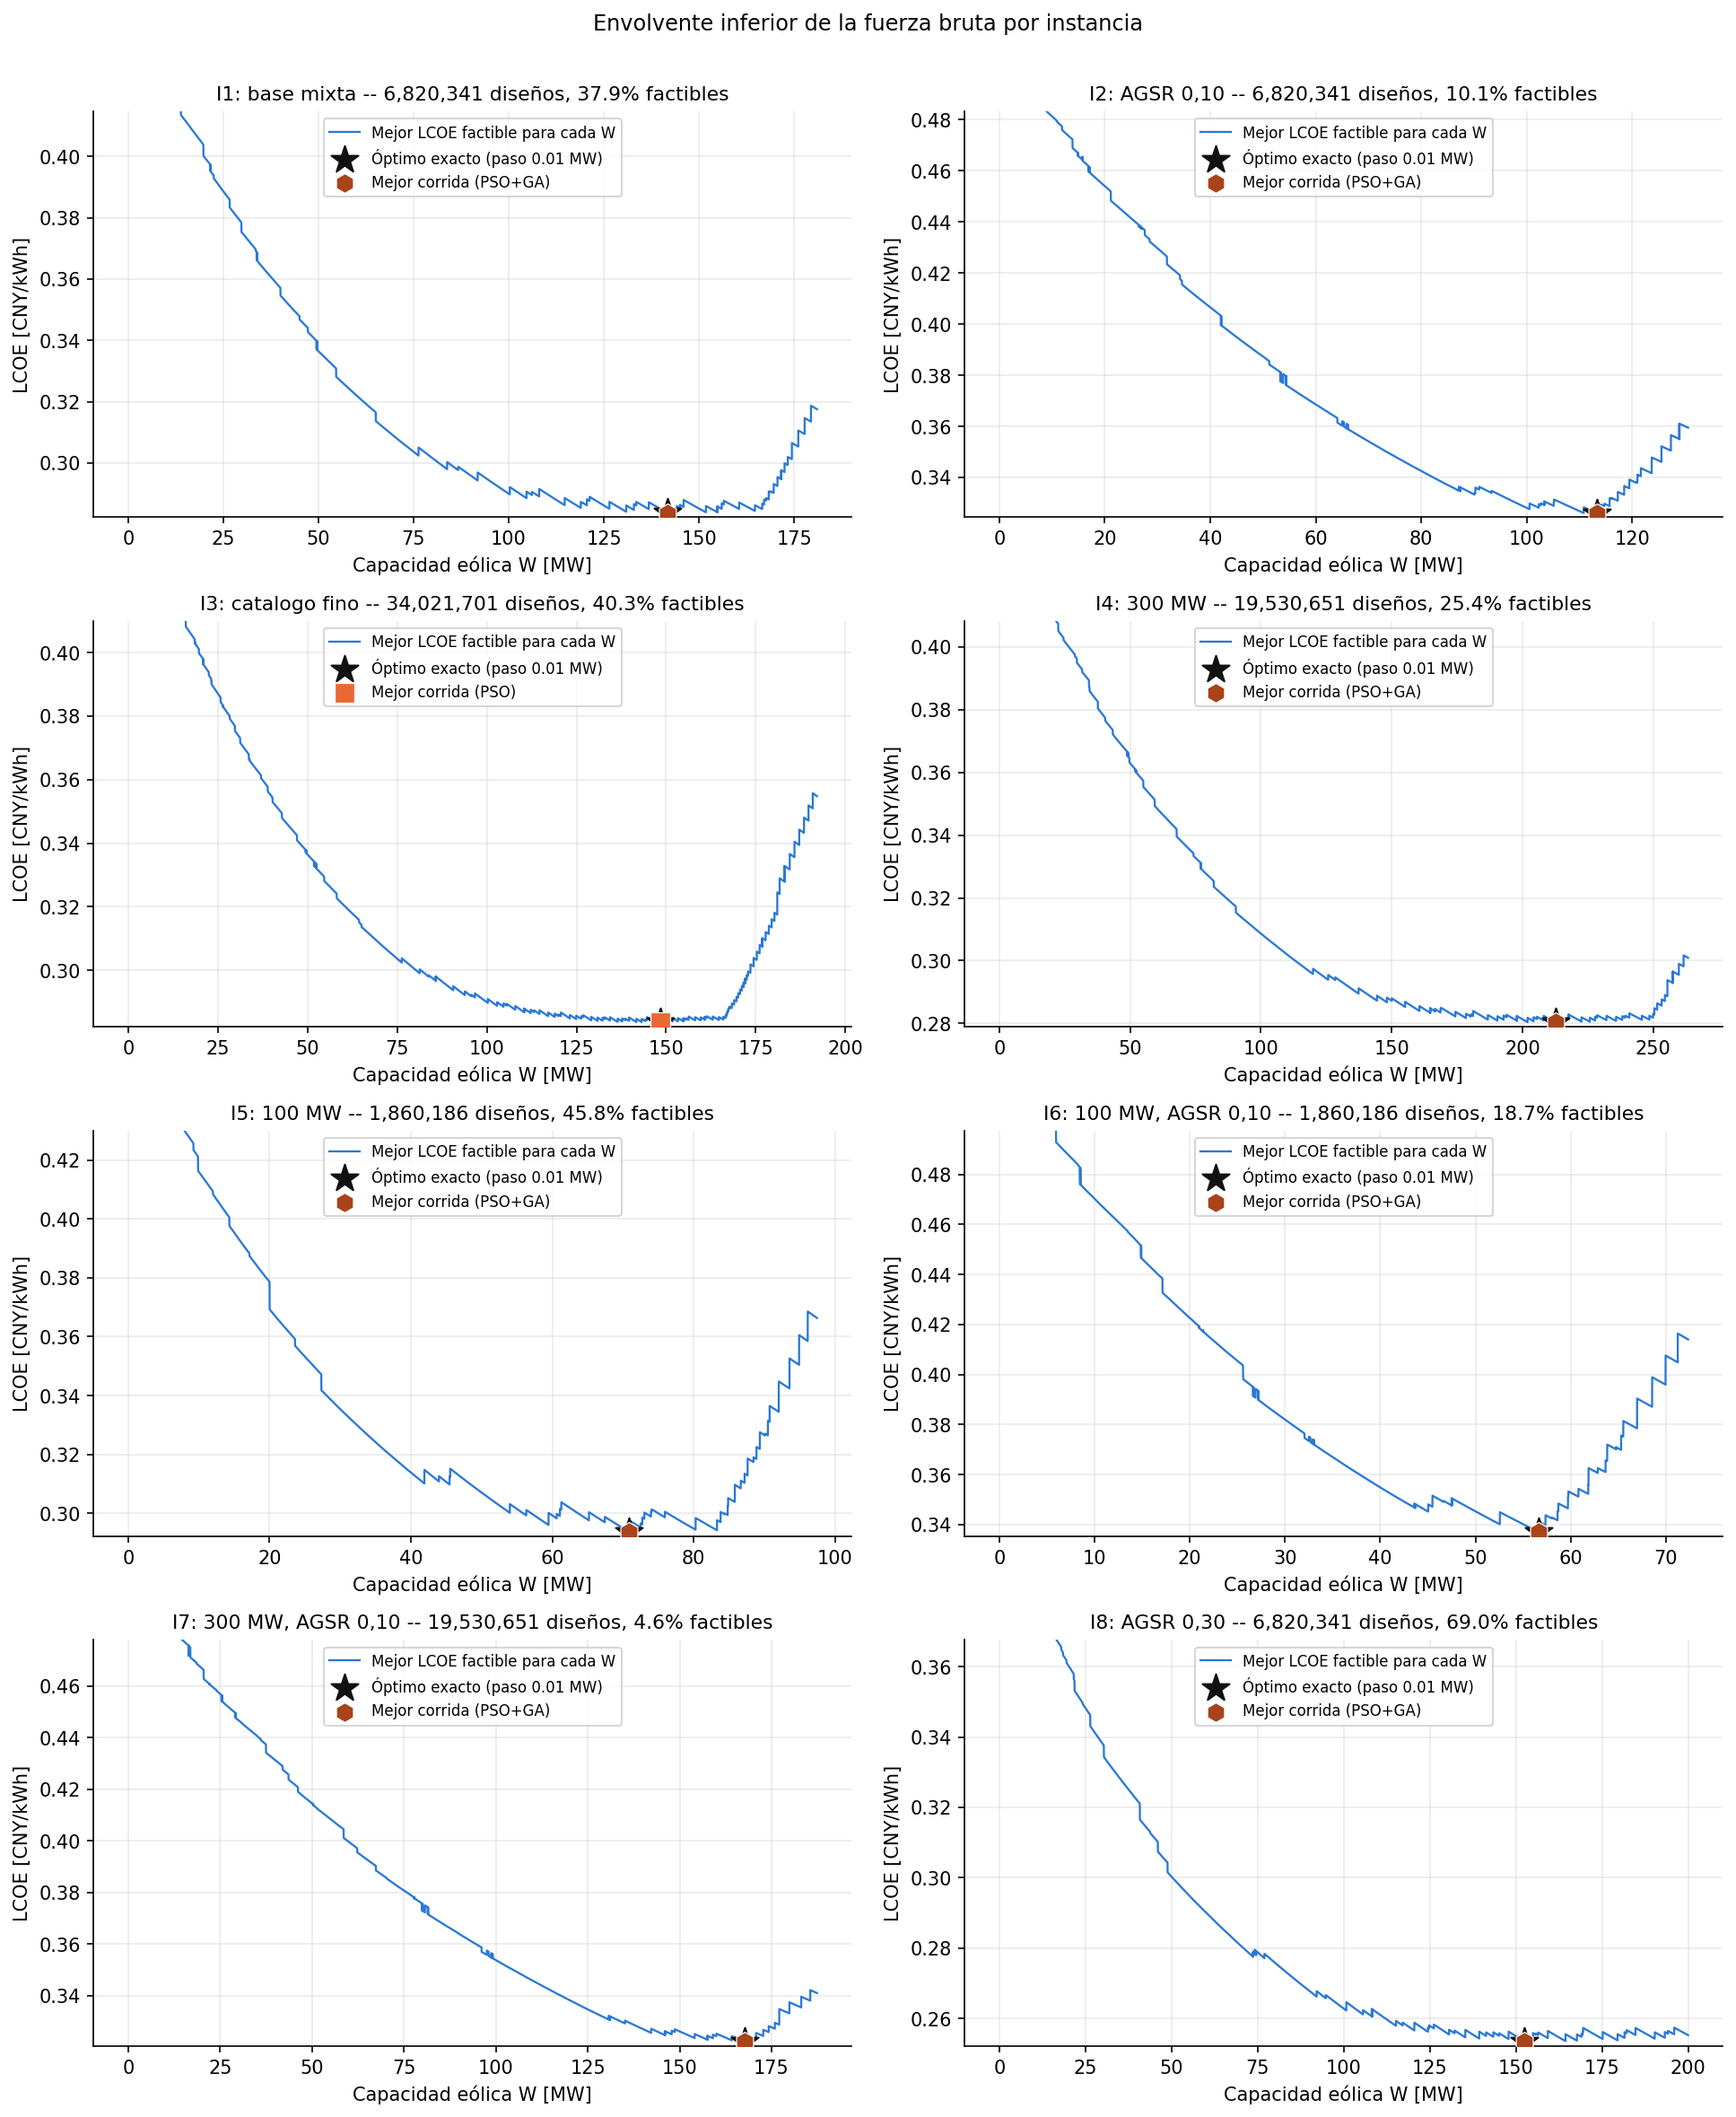
\includegraphics[width=0.98\textwidth]{figures/fig10_envolvente_fuerza_bruta.png}
\caption{Envolvente inferior de la fuerza bruta por instancia: mejor LCOE factible entre todos los catálogos para cada valor de $W$. La estrella es el óptimo exacto y el marcador coloreado la mejor corrida estocástica de la instancia.}
\label{fig:envolvente}
\end{figure}

La Figura~\ref{fig:envolvente} muestra la geometría que los algoritmos deben recorrer: la envolvente sólo existe donde hay diseños factibles, desciende suavemente hasta el óptimo y termina abruptamente en el borde de C5. La Tabla~\ref{tab:comparacion_optimo_auto} compara el óptimo exacto con la mejor corrida estocástica de cada instancia; las brechas son de \BestRunAGapPct\,\% (I1, \BestRunAAlgorithm), \BestRunBGapPct\,\% (I2, \BestRunBAlgorithm), \BestRunCGapPct\,\% (I3, \BestRunCAlgorithm) y \BestRunDGapPct\,\% (I4, \BestRunDAlgorithm). Una brecha negativa significa que el optimizador, con $W$ continuo, halló un diseño entre dos nodos de la malla de 0,01 MW.

\TablaComparacionOptimoAuto

\section{Comparación de los optimizadores por instancia}

Se ejecutaron \TotalRuns{} corridas y \TotalDesignRequests{} solicitudes de evaluación de diseños anuales. Cada una recorre 8.760 pasos horarios, por lo que el total solicitado equivale aproximadamente a \RequestedHourlySteps{} pasos; las propuestas duplicadas se contabilizan dentro del presupuesto aunque la memoria intermedia evite repetir la simulación. Las Figuras~\ref{fig:convergencia} y~\ref{fig:dispersion} muestran la convergencia y la distribución final en las cuatro instancias; las tablas siguientes detallan cada una.

\begin{figure}[H]
\centering
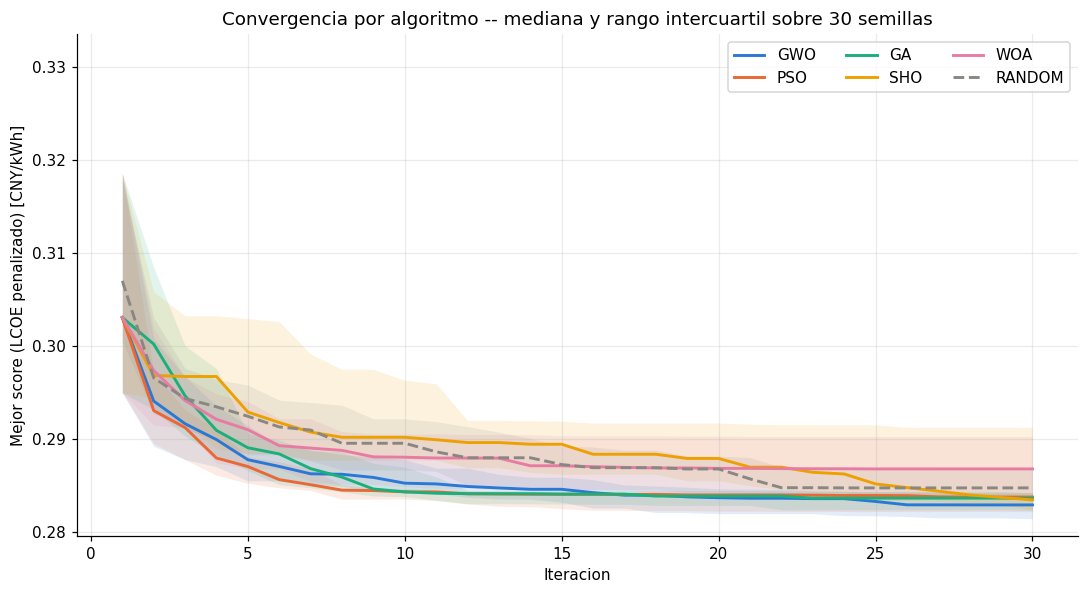
\includegraphics[width=0.98\textwidth]{figures/fig05_convergencia.png}
\caption{Mediana e intervalo intercuartílico del mejor LCOE factible a igual número de solicitudes, por instancia. La línea punteada es el óptimo exacto.}
\label{fig:convergencia}
\end{figure}

\begin{figure}[H]
\centering
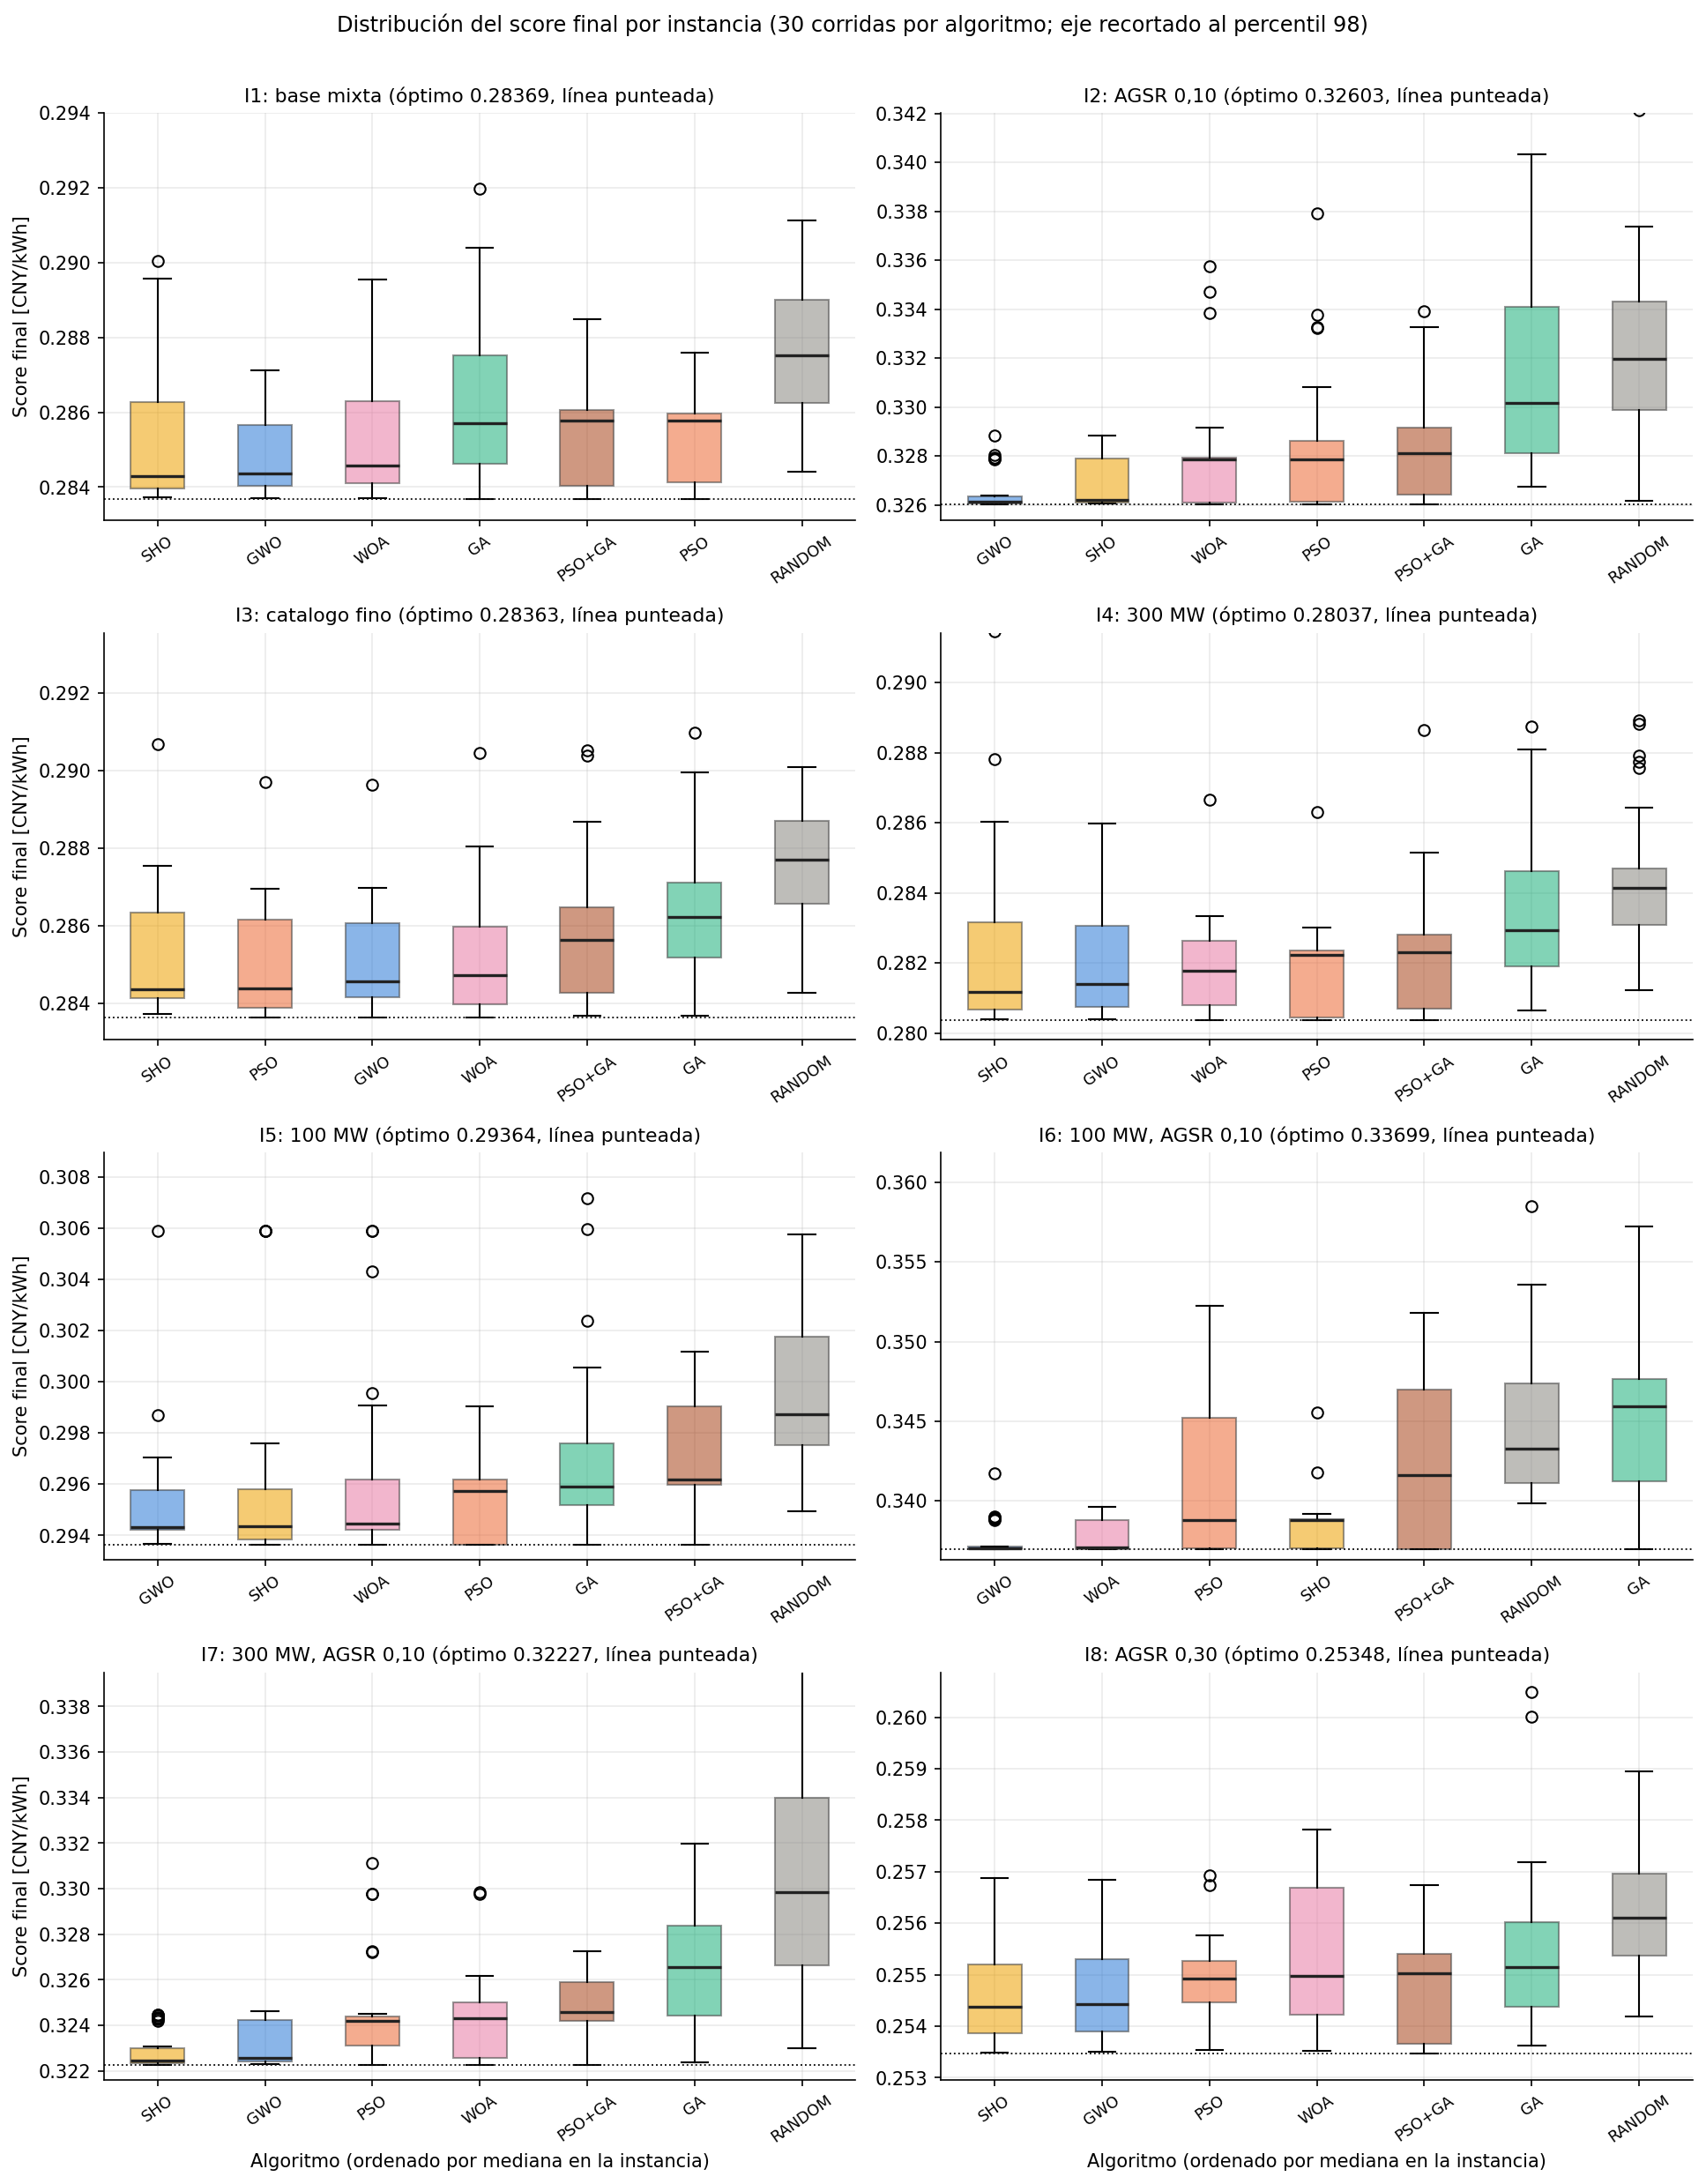
\includegraphics[width=0.98\textwidth]{figures/fig06_distribucion_scores.png}
\caption{Distribución del LCOE final de las \Replicates{} ejecuciones independientes por algoritmo e instancia, ordenadas por mediana dentro de cada instancia.}
\label{fig:dispersion}
\end{figure}

\subsection{I1: instancia mixta de referencia}

\TablaRankingAutoA
\TablaExitoAutoA
\TablaComputoAutoA
\TablaParesPlanificadosAutoA

Por mediana, \TopMedianA{} ocupa la primera posición con una brecha mediana de \TopMedianGapA\,\% respecto del óptimo exacto, seguido de \SecondMedianA; \BottomMedianA{} ocupa la última y la búsqueda aleatoria el lugar \RandomRankA{} con brecha mediana de \RandomMedianGapA\,\%. Frente a esa línea base, muestran ventaja detectable tras Holm \BetterThanRandomA; sin diferencia detectable, \NoDifferenceFromRandomA; con desventaja detectable, \WorseThanRandomA. Esta última categoría expresa ausencia de evidencia y no igualdad algorítmica. Entre los híbridos, superan la mediana de su padre \HybridsBeatParentA; los contrastes híbrido--padre significativos son \HybridsSignificantA.

\subsection{I2: región factible estrecha}

\TablaRankingAutoB
\TablaExitoAutoB
\TablaComputoAutoB
\TablaParesPlanificadosAutoB

Con el límite de ventas a red reducido a la mitad, \TopMedianB{} ocupa la primera posición (brecha mediana \TopMedianGapB\,\%), seguido de \SecondMedianB; \BottomMedianB{} ocupa la última y la búsqueda aleatoria el lugar \RandomRankB{} (brecha mediana \RandomMedianGapB\,\%). Ventaja detectable frente a la línea base: \BetterThanRandomB; sin diferencia detectable: \NoDifferenceFromRandomB; desventaja detectable: \WorseThanRandomB. Superan la mediana de su padre \HybridsBeatParentB; contrastes híbrido--padre significativos: \HybridsSignificantB. Como mínimo \FeasibleRunsMinB{} de las \Replicates{} corridas de cada algoritmo terminaron en un diseño factible.

\subsection{I3: catálogos finos}

\TablaRankingAutoC
\TablaExitoAutoC
\TablaComputoAutoC
\TablaParesPlanificadosAutoC

Con cinco veces más combinaciones discretas sobre la misma región física, \TopMedianC{} ocupa la primera posición (brecha mediana \TopMedianGapC\,\%), seguido de \SecondMedianC; \BottomMedianC{} ocupa la última y la búsqueda aleatoria el lugar \RandomRankC{} (brecha mediana \RandomMedianGapC\,\%). Ventaja detectable frente a la línea base: \BetterThanRandomC; sin diferencia detectable: \NoDifferenceFromRandomC; desventaja detectable: \WorseThanRandomC. Superan la mediana de su padre \HybridsBeatParentC; contrastes híbrido--padre significativos: \HybridsSignificantC.

\subsection{I4: escala de 300 MW}

\TablaRankingAutoD
\TablaExitoAutoD
\TablaComputoAutoD
\TablaParesPlanificadosAutoD

A escala de 300 MW, \TopMedianD{} ocupa la primera posición (brecha mediana \TopMedianGapD\,\%), seguido de \SecondMedianD; \BottomMedianD{} ocupa la última y la búsqueda aleatoria el lugar \RandomRankD{} (brecha mediana \RandomMedianGapD\,\%). Ventaja detectable frente a la línea base: \BetterThanRandomD; sin diferencia detectable: \NoDifferenceFromRandomD; desventaja detectable: \WorseThanRandomD. Superan la mediana de su padre \HybridsBeatParentD; contrastes híbrido--padre significativos: \HybridsSignificantD.

\section{Lectura transversal}

\TablaRankingTransversalAuto

El rango medio sobre las cuatro instancias sitúa en primer lugar a \BestMeanRankAlgorithm{} (rango medio \BestMeanRank) y en segundo a \SecondMeanRankAlgorithm{} (\SecondMeanRank); \WorstMeanRankAlgorithm{} ocupa el último lugar y la búsqueda aleatoria obtiene un rango medio de \RandomMeanRank. El orden es descriptivo: resume cuatro instancias paramétricas del mismo sitio y año, no una población de problemas, y las diferencias de rango entre algoritmos vecinos no son evidencia de superioridad. Las columnas de brecha y éxito medios permiten leer el mismo cuadro en términos prácticos: cuán lejos del óptimo queda una corrida típica y con qué frecuencia queda a menos de 0,5\,\% de él.

Los mecanismos de movimiento ofrecen hipótesis para interpretar las curvas: memoria personal y social en PSO, tres líderes en GWO, recombinación en GA, cambios de rama o agrupación en WOA y SHO, intensificación local en GA+LS y SHO+LS, y diversidad estructurada en PSO+GA. Sin embargo, el experimento sólo contiene ablaciones para el componente añadido por cada híbrido; en los clásicos la explicación causal por operador se mantiene como vacío metodológico, no como conclusión demostrada.

\section{Híbridos frente a sus padres}

\TablaHibridosAuto

\begin{figure}[H]
\centering
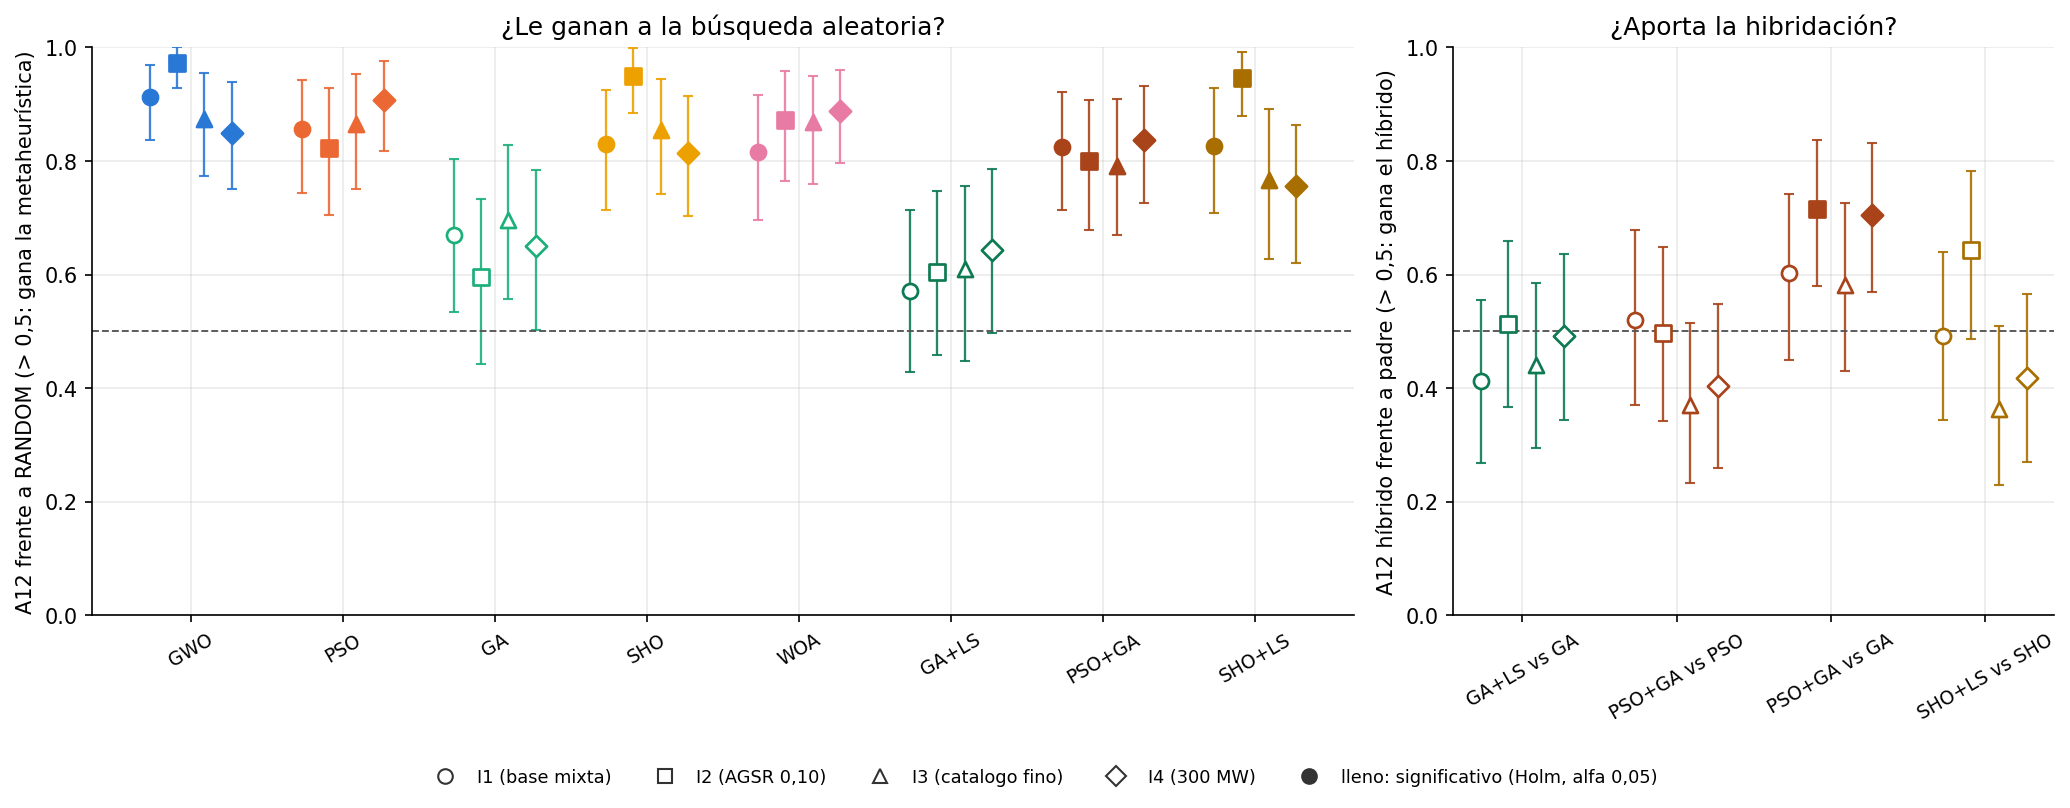
\includegraphics[width=0.98\textwidth]{figures/fig07_contrastes_planificados.png}
\caption{Contrastes planificados: $A_{12}$ con intervalo bootstrap al 95\,\% de cada metaheurística frente a RANDOM (izquierda) y de cada híbrido frente a su padre (derecha), por instancia. Marcador lleno: significativo tras Holm en la familia de la instancia.}
\label{fig:contrastes}
\end{figure}

La pregunta central de la extensión es si la hibridación aporta algo respecto del método del que parte. De los \HybridContrastsTotal{} contrastes híbrido--padre (cuatro por instancia), el híbrido obtiene mejor mediana que su padre en \HybridWinsCount{} y la diferencia es significativa tras Holm en \HybridSignificantCount{}: \HybridSignificantWins{} a favor del híbrido y \HybridSignificantLosses{} en su contra. La Tabla~\ref{tab:hibridos_auto} y la Figura~\ref{fig:contrastes} muestran que el efecto depende del par y de la instancia, lo que es coherente con el teorema de la no existencia de almuerzo gratis: añadir una búsqueda local o un operador genético redistribuye el presupuesto entre exploración y explotación, y el saldo de esa redistribución cambia con la geometría de la región factible. Las columnas de solicitudes de búsqueda local de las tablas de cómputo cuantifican cuánto presupuesto consumió la intensificación en cada instancia.

Tres patrones concretos se desprenden de la tabla. Primero, los dos contrastes significativos corresponden a PSO+GA frente a GA (I2 e I4), ambos a favor del híbrido, mientras que PSO+GA frente a PSO no se distingue en ninguna instancia ($A_{12}$ entre 0,37 y 0,52): el híbrido hereda la calidad del bucle del enjambre, y reemplazar el cuarto peor de las partículas por hijos genéticos ni mejora ni empeora al PSO puro bajo este presupuesto. Segundo, SHO+LS ocupa el primer lugar por mediana en I2, la instancia de región factible estrecha, y supera a SHO en mediana sólo allí; en I3 e I4 cae al sexto lugar. La búsqueda local consume entre 66 y 69 solicitudes por corrida, un 11\,\% del presupuesto, que en una región estrecha se invierten en afinar $W$ sobre el borde de C5 y que en un espacio discreto cinco veces mayor se restan a la exploración. Tercero, GA+LS no mejora a GA en ninguna instancia de forma detectable: parte de un método cuyo presupuesto ya se gasta en más de un 30\,\% en diseños repetidos (unas 180 a 207 solicitudes duplicadas por corrida en GA, 143 a 153 en GA+LS), y la búsqueda local añade cerca de 97 solicitudes más de intensificación sobre un individuo que el elitismo ya conserva. Las mejores corridas individuales de I1, I2 e I4 corresponden, sin embargo, a PSO+GA, y la de I3 a PSO, todas por debajo del óptimo discretizado gracias a $W$ continuo.

\section{Análisis de sensibilidad}

\TablaSensAGSRAuto
\TablaSensCargaAuto

\begin{figure}[H]
\centering
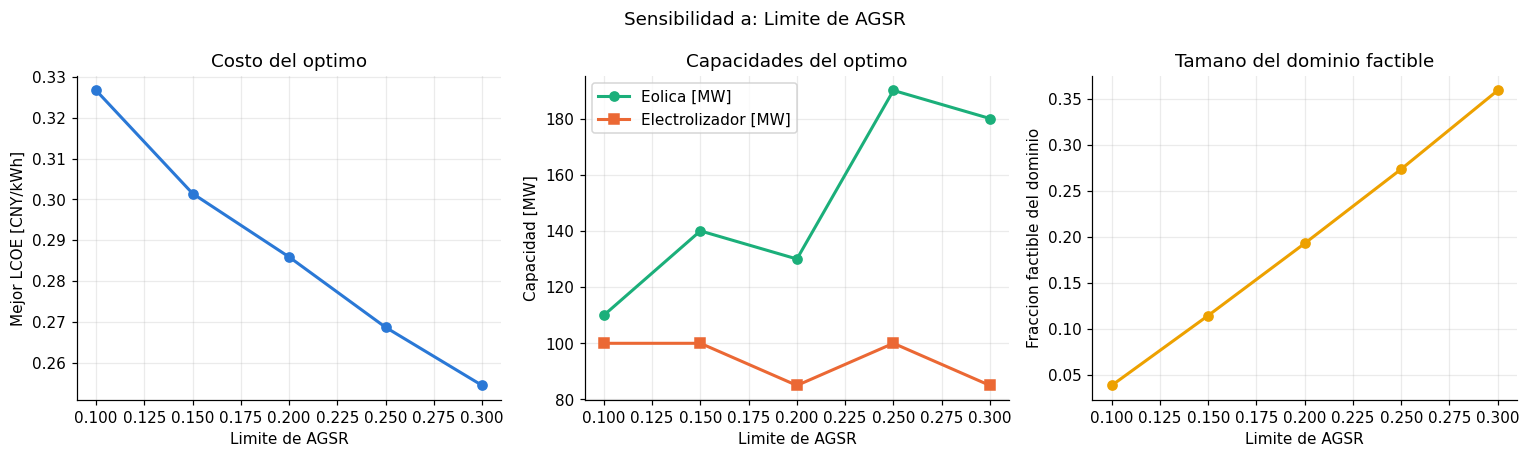
\includegraphics[width=0.96\textwidth]{figures/fig08_sensibilidad_agsr.png}
\caption{Sensibilidad determinista de la malla base al límite de fracción anual vendida a red.}
\label{fig:sens_agsr}
\end{figure}

\begin{figure}[H]
\centering
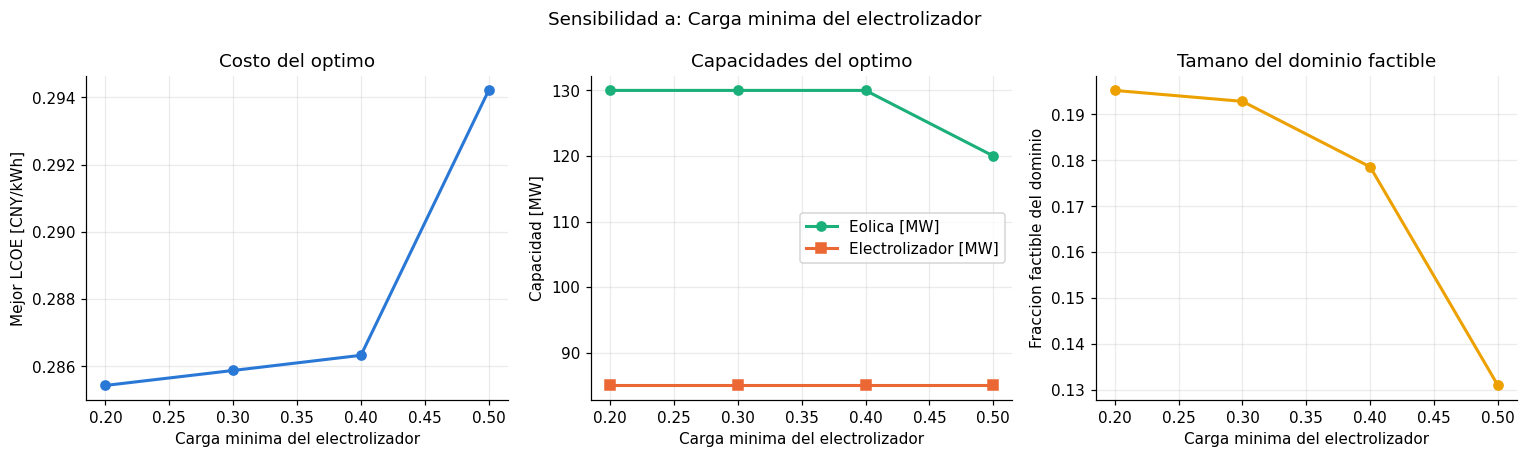
\includegraphics[width=0.96\textwidth]{figures/fig09_sensibilidad_carga_minima.png}
\caption{Sensibilidad determinista de la malla base a la carga mínima del electrolizador.}
\label{fig:sens_carga}
\end{figure}

Los barridos separan el efecto de las restricciones del ruido de los optimizadores. Muestran cómo cambian simultáneamente el tamaño de la región factible y el mejor punto de la malla base; no constituyen una prueba de robustez del ranking algorítmico. El barrido del límite de AGSR anticipa, sobre la malla base, el estrechamiento que la instancia I2 impone al dominio mixto.

\section{Verificaciones y alcance de los resultados}

Las \TotalRuns{} corridas registraron exactamente \RequestsPerRun{} solicitudes cada una y el residuo máximo de balance observado fue \texttt{\MaxBalanceResidual} MW; como mínimo \MinFeasibleRuns{} de las \Replicates{} corridas de cada algoritmo e instancia terminaron en un diseño factible. GWO, SHO, WOA y la inyección genética de PSO+GA superaron pruebas de una actualización determinista contra sus ecuaciones; la búsqueda local superó las pruebas de convergencia, presupuesto y ausencia de duplicados; los tres híbridos produjeron exactamente \Iterations{} puntos de control por corrida; y clásicos e híbridos superaron las pruebas de dirección y límites sobre Sphere y Rastrigin. La corrida de I1 reproduce bit a bit la comparativa previa de seis algoritmos.

Los resultados continúan condicionados por un solo emplazamiento aproximado y un solo año meteorológico; por instancias que varían una restricción, la finura de los catálogos y la escala, pero no el recurso ni la estructura de costos; por la ausencia de una demanda explícita de hidrógeno; por la idealización continua de $W$; por la regla declarada para operacionalizar la agrupación de SHO; y por valores de la búsqueda local y de la inyección genética fijados a priori y sin ablación por operador. El experimento compara implementaciones concretas bajo un presupuesto concreto, no familias algorítmicas en general.

\chapter{Conclusiones}

\section{Cumplimiento de los objetivos}

El trabajo desarrollado permite evaluar el grado de cumplimiento de cada uno de los objetivos específicos planteados.

El \textbf{análisis de la estructura matemática} del modelo WPEB (objetivo 1) se materializó en la formulación completa recogida en el marco teórico, que identifica las variables de decisión, las cinco restricciones operacionales, los modelos de conversión eólica y fotovoltaica, la dinámica del almacenamiento y los cuatro indicadores económicos del sistema.

La \textbf{implementación y verificación} del modelo (objetivo 2) se completó con un resultado de nueve indicadores dentro de tolerancia sobre diez contrastados. El proceso de verificación aportó además dos hallazgos no previstos: la tabla de costos del artículo de referencia resulta internamente inconsistente en uno de sus casos de comparación, y la configuración que dicho artículo presenta como óptima es infactible bajo la restricción de venta a red que él mismo establece, con un valor de 0,270 frente a un límite declarado de 0,20.

La \textbf{evaluación crítica de los supuestos} (objetivo 3) condujo a tres decisiones de modelado documentadas con evidencia empírica: la adopción de la serie de viento medida a 50 m frente a su extrapolación a altura de buje, la corrección de la interpretación de la irradiancia --- cuyo efecto sobre el factor de capacidad fotovoltaico fue de dos órdenes de magnitud --- y el reparto del costo de la batería entre componentes de potencia y de energía.

La \textbf{formulación de la instancia discreta} (objetivo 4) amplió el dominio admisible de 420 a 14.883 configuraciones, incorporando la potencia y la duración del almacenamiento como variables de diseño, con una estrategia mixta de proyección y penalización proporcional para el tratamiento de restricciones.

La \textbf{comparación entre metaheurísticas} (objetivo 5) se ejecutó sobre 108.000 simulaciones horarias, con las 180 corridas concluyendo en soluciones factibles. La \textbf{significancia estadística} (objetivo 6) se estableció mediante contrastes de Wilcoxon con corrección de Holm--Bonferroni y tamaños de efecto $A_{12}$, identificando cinco pares distinguibles de quince. El \textbf{análisis de sensibilidad y robustez} (objetivo 7) cuantificó la influencia de las dos restricciones operacionales y demostró la inestabilidad del ranking frente a una decisión de modelado.

El objetivo 8, relativo al \textbf{establecimiento de bases para una formulación multiobjetivo}, se cumple parcialmente: el simulador calcula ya los indicadores necesarios y la arquitectura del software admite la sustitución de la función de aptitud, pero la formulación multiobjetivo propiamente dicha queda como línea de trabajo futuro.

\section{Conclusiones sobre el problema de dimensionamiento}

El dimensionamiento óptimo del sistema estudiado está gobernado por una restricción regulatoria y no tecnológica. El límite sobre la fracción anual de energía vendida a la red determina la ubicación del óptimo con una influencia un orden de magnitud superior a la de la carga mínima del electrolizador: relajarlo del 10\,\% al 30\,\% reduce el costo nivelado óptimo en 0,0723 CNY/kWh, mientras que variar la carga mínima entre el 20\,\% y el 50\,\% lo altera en 0,0088 CNY/kWh. El óptimo se sitúa siempre sobre la frontera de esa restricción, porque el costo nivelado decrece con la capacidad eólica mientras la fracción vendida a la red crece con ella.

El paisaje de optimización presenta una meseta de soluciones prácticamente equivalentes a lo largo de dicha frontera. Las cuatro mejores configuraciones de la instancia base difieren en menos del 0,5\,\% de costo nivelado pese a cubrir un rango de 30 MW de capacidad eólica. Esta característica tiene una consecuencia directa sobre la elección del optimizador, que se aborda a continuación.

\section{Conclusiones sobre el desempeño de las metaheurísticas}

Sobre la instancia discreta estudiada, la evidencia sostiene cuatro conclusiones.

\textbf{Primera: las diferencias entre algoritmos son estadísticamente detectables pero prácticamente marginales.} Los seis optimizadores alcanzan valores comprendidos en un rango del 0,25\,\%, y solo cinco de quince pares resultan distinguibles tras la corrección por comparaciones múltiples. En un problema con la estructura descrita, la elección del algoritmo importa considerablemente menos de lo que sugiere la literatura.

\textbf{Segunda: la consistencia es un criterio más informativo que el mejor valor alcanzado.} El algoritmo genético obtuvo el mejor resultado absoluto del experimento y, sin embargo, no se distingue estadísticamente de la búsqueda aleatoria. PSO y GWO, con desviaciones típicas de 0,001426 y 0,001595, son las opciones defendibles para un uso real, en el que el optimizador se ejecuta una sola vez y lo que importa es el resultado esperable de una ejecución cualquiera, no el mejor de treinta.

\textbf{Tercera: dos de las cinco metaheurísticas no superan a la búsqueda aleatoria.} WOA queda por debajo de la línea base en mejor valor, en media y en consistencia, con una desviación típica más de tres veces superior a la de PSO. SHO no se distingue estadísticamente de ella y presenta un modo de fallo identificable, consistente en converger a configuraciones sin almacenamiento. Ninguno de los dos justifica su complejidad adicional en este problema.

\textbf{Cuarta: el ordenamiento entre algoritmos no es una propiedad de los algoritmos.} Al fijar la duración de la batería en una hora e imputar su costo íntegramente a la potencia, el algoritmo genético desciende del primer al cuarto lugar y WOA asciende del sexto al tercero, mientras el número de pares significativos pasa de cinco a ocho. Lo que se mide al comparar metaheurísticas es el comportamiento de la pareja algoritmo--formulación, y un ranking reportado sin análisis de robustez afirma más de lo que sus datos respaldan.

\section{Aporte a la Ingeniería Informática}

La contribución de este trabajo a la disciplina se articula en cuatro ejes.

\subsection{Aporte metodológico}

El trabajo propone y aplica un protocolo reproducible para la comparación empírica de metaheurísticas sobre problemas de ingeniería con evaluación costosa, construido sobre cinco requisitos: equiparación del presupuesto de evaluaciones como unidad de comparación, inclusión obligatoria de una línea base no informada, diseño pareado por semilla que permite descontar el efecto de la inicialización, contrastes no paramétricos con control de la tasa de error por familia, y verificación de la estabilidad del ordenamiento frente a las decisiones de modelado.

Ninguno de estos elementos es original por separado; su valor reside en su aplicación conjunta y sistemática a un problema de ingeniería real, y en la demostración de que su omisión conduce a conclusiones distintas. El protocolo es transferible a cualquier problema de dimensionamiento o de optimización de caja negra con evaluación costosa, y no depende del dominio energético.

\subsection{Aporte empírico}

El hallazgo central es de signo negativo, y ese es precisamente su valor. En un problema representativo del dominio, dos metaheurísticas ampliamente citadas y aplicadas no superan a un muestreo uniforme del espacio de búsqueda. Este resultado no contradice la teoría --- es de hecho lo que anticipa el teorema de la no existencia de almuerzo gratis \cite{Wolpert1997NFL} --- pero contradice una práctica extendida: la adopción de algoritmos bioinspirados por su popularidad o por la elegancia de su metáfora, sin verificar que aporten algo sobre una referencia trivial.

Los resultados negativos están sistemáticamente subrepresentados en la literatura de metaheurísticas, sesgo que dificulta la acumulación de conocimiento fiable sobre qué algoritmos funcionan y en qué condiciones. Reportar este hallazgo, en lugar de seleccionar la configuración experimental que hubiera favorecido una conclusión positiva, constituye una contribución en sí misma.

\subsection{Aporte a la replicabilidad}

La réplica verificada de un artículo indexado, con nueve de diez indicadores dentro de tolerancia, aporta a la comunidad un modelo cuya corrección está establecida y no supuesta. Durante el proceso se detectaron dos problemas en el artículo original: una inconsistencia interna en su tabla de costos, y la infactibilidad de su configuración óptima respecto de su propia restricción operacional.

El caso ilustra además un punto metodológico de alcance general. El error de interpretación de la irradiancia detectado durante la verificación no producía excepciones ni resultados manifiestamente absurdos: el simulador entregaba costos nivelados plausibles mientras la producción fotovoltaica era prácticamente nula. Solo el contraste cuantitativo sistemático contra indicadores publicados permitió descubrirlo. En software científico, la ausencia de errores visibles no constituye evidencia de corrección.

\subsection{Aporte en ingeniería de software científico}

Las decisiones de arquitectura adoptadas --- configuración inmutable con validación en construcción, separación entre la definición de la instancia y la estrategia de búsqueda mediante una clase base con contrato explícito, registro extensible de optimizadores, memoización de perfiles de generación y ejecución conmutable entre dos escalas de presupuesto --- son las que hacen el experimento auditable y reproducible.

La decisión de mantener el artefacto computacional autocontenido, sin dependencias de una estructura de paquetes propia, permite que la totalidad de los resultados de esta tesis sea reproducible a partir de dos archivos. Esta propiedad, habitualmente sacrificada en favor de la modularidad, resulta especialmente valiosa en el contexto de un trabajo académico destinado a ser verificado por terceros.

\section{Limitaciones}

Los resultados deben interpretarse dentro de los siguientes límites, declarados de forma explícita.

\begin{itemize}
    \item \textbf{Alcance del sistema modelado.} El sistema WPEB no incluye pila de combustible ni reelectrificación del hidrógeno, por lo que no constituye una cadena HRES-H$_2$ completa. El almacenamiento de hidrógeno se fija en 10.000 kg y no es variable de decisión.

    \item \textbf{Formulación monoobjetivo.} Se optimiza exclusivamente el costo nivelado de la energía. El costo nivelado del hidrógeno y el costo presente neto se reportan pero no intervienen en la función de aptitud, y no se consideran criterios ambientales ni de confiabilidad.

    \item \textbf{Capacidad renovable total fija.} La suma de capacidad eólica y fotovoltaica permanece fija en 200 MW, restricción heredada del modelo de referencia que impide explorar el compromiso entre tamaño total del sistema y costo unitario.

    \item \textbf{Un único año meteorológico.} Los resultados se basan en el año 2008. No se evalúa la variabilidad interanual del recurso ni la robustez de las soluciones frente a años meteorológicos distintos.

    \item \textbf{Ausencia de demanda explícita de hidrógeno.} Se asume que la totalidad del hidrógeno producido encuentra colocación, sin perfil de demanda ni restricciones de logística o de precio.

    \item \textbf{Hiperparámetros sin ajuste fino.} Los algoritmos emplean los valores canónicos de sus publicaciones originales. Un ajuste específico para este problema podría modificar el ordenamiento, si bien tal ajuste requeriría un presupuesto computacional propio que debería contabilizarse en la comparación.

    \item \textbf{Escala del problema.} Con 600 evaluaciones sobre 14.883 configuraciones, el dominio resulta lo bastante pequeño para que la búsqueda aleatoria sea competitiva. Las conclusiones sobre desempeño relativo no son extrapolables a instancias de mayor dimensionalidad sin verificación adicional.

    \item \textbf{Coordenadas aproximadas del emplazamiento.} El artículo de referencia no publica la latitud y longitud exactas, por lo que el recurso meteorológico empleado es una aproximación razonable pero no idéntica al del estudio original.
\end{itemize}

\section{Trabajo futuro}

Las líneas de continuación se ordenan por su proximidad a lo ya desarrollado.

\textbf{Escalado de la instancia.} La limitación más relevante de este trabajo es que el problema resulta demasiado sencillo para discriminar entre optimizadores. Liberar la capacidad renovable total, incorporar el dimensionamiento del almacenamiento de hidrógeno y añadir una etapa de compresión elevaría la dimensionalidad hasta un régimen donde la enumeración deje de ser viable y donde las diferencias entre metaheurísticas puedan manifestarse con magnitud práctica.

\textbf{Formulación multiobjetivo.} La extensión natural consiste en optimizar simultáneamente el costo nivelado de la energía, el costo nivelado del hidrógeno y un indicador de emisiones evitadas, mediante algoritmos de frente de Pareto como NSGA-II o MOPSO. El simulador ya calcula los indicadores necesarios y la arquitectura del software admite la sustitución de la función de aptitud sin modificaciones estructurales.

\textbf{Hibridación con componentes de aprendizaje.} La integración de redes neuronales artificiales como modelos sustitutos de la función objetivo permitiría reducir el número de simulaciones horarias requeridas, aprovechando que el costo dominante del problema es precisamente la evaluación. Esta línea resulta particularmente pertinente una vez escalada la instancia.

\textbf{Optimización de la memoización.} La cuantización de la capacidad eólica a una malla fina elevaría la tasa de acierto de la memoria intermedia del 18,2\,\% actual a valores superiores al 95\,\%, reduciendo sustancialmente el tiempo de experimentación sin alterar apreciablemente la resolución del espacio de búsqueda.

\textbf{Robustez frente a la variabilidad del recurso.} Evaluar las soluciones óptimas sobre múltiples años meteorológicos permitiría distinguir los diseños genuinamente robustos de aquellos ajustados a las particularidades de un año concreto, incorporando la incertidumbre del recurso al propio proceso de optimización.


\clearpage
\printbibliography[title={Referencias bibliográficas}, heading=bibintoc]

\appendix
\chapter{Identidad visual de los algoritmos}

Las figuras comparativas de este documento emplean una codificación visual consistente: cada algoritmo mantiene el mismo color y el mismo marcador en todas las representaciones, de modo que el lector pueda seguir un competidor concreto a través de las distintas figuras sin recurrir a la leyenda en cada caso.

\begin{figure}[H]
\centering
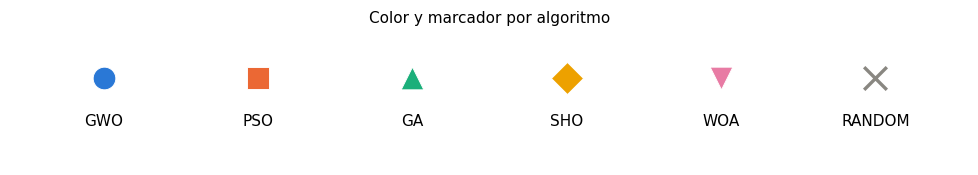
\includegraphics[width=0.82\textwidth]{figures/fig04_identidad_visual.png}
\caption{Correspondencia entre algoritmo, color y marcador empleada de forma consistente en todas las figuras comparativas.}
\label{fig:identidad_visual}
\end{figure}

La forma del marcador actúa como codificación primaria y el color como refuerzo secundario. Esta redundancia evita que la identificación de nueve series dependa exclusivamente de la percepción cromática y mantiene la lectura al imprimir en escala de grises. Los tres híbridos heredan el tono de su padre y se distinguen por un patrón de línea de puntos y rayas y por un marcador propio.

\chapter{Plan de trabajo del proyecto}

El trabajo recogido en esta tesis corresponde a la ejecución completa del primer paquete de trabajo de un proyecto de investigación de mayor alcance, cuya estructura se documenta aquí para situar el aporte realizado.

\section{WP1: Evaluación de metaheurísticas para HRES-H$_2$}

Su propósito es evaluar la aplicabilidad, flexibilidad y limitaciones de las metaheurísticas de población aplicadas a configuraciones HRES-H$_2$, identificando las características críticas del problema y las limitaciones de los enfoques existentes.

\begin{itemize}
    \item \textbf{Tarea 1.1:} revisión del estado del arte sobre modelos HRES-H$_2$ y análisis de su complejidad computacional. \textit{Completada}, véase el marco teórico.
    \item \textbf{Tarea 1.2:} revisión del estado del arte sobre metaheurísticas modernas basadas en población. \textit{Completada}, con la incorporación de GWO \cite{Mirjalili2014GWO}, PSO \cite{Kennedy1995PSO}, GA \cite{Goldberg1989GA}, SHO \cite{Dhiman2017SHO} y WOA \cite{Mirjalili2016WOA}.
    \item \textbf{Tarea 1.3:} análisis de enfoques híbridos de optimización basados en población. \textit{Completada}, con la taxonomía de Talbi \cite{Talbi2002Taxonomy} y tres híbridos integrativos de bajo nivel: GA+LS \cite{Moscato1989Memetic}, PSO+GA \cite{Kao2008HybridGAPSO} y SHO+LS. La integración de componentes de aprendizaje se traslada al WP2.
    \item \textbf{Tarea 1.4:} implementación, experimentación y evaluación de los enfoques seleccionados. \textit{Completada} para las cuatro instancias y las sensibilidades declaradas; véanse los capítulos de diseño experimental y de resultados.
\end{itemize}

\section{WP2: Integración de componentes de aprendizaje basados en ANN}

Orientado al diseño e integración de redes neuronales artificiales dentro de marcos de optimización híbrida, con el objetivo de reducir el número de evaluaciones costosas mediante modelos sustitutos de la función objetivo. Su pertinencia queda reforzada por los resultados de esta tesis: siendo la simulación horaria el costo dominante, un modelo sustituto suficientemente preciso permitiría ampliar el presupuesto efectivo de búsqueda en órdenes de magnitud.

\section{WP3: Extensión ambiental y multiobjetivo}

Aborda la incorporación de métricas de sostenibilidad al proceso de optimización, complementando los criterios técnicos y económicos con indicadores ambientales bajo una formulación multiobjetivo de frente de Pareto.

\section{WP4: Difusión y comunicación de resultados}

Contempla la comunicación de los avances metodológicos y de los resultados obtenidos a audiencias académicas y técnicas.

\chapter{Reproducibilidad del experimento}

\section{Artefactos computacionales}

La totalidad de los resultados reportados en esta tesis se regenera a partir de los siguientes artefactos:

\begin{itemize}
    \item \texttt{notebooks/H2\_HRES\_trabajo.ipynb} --- cuaderno autocontenido de 22 secciones que incluye configuración, modelos físicos y económicos, pruebas deterministas, reproducción parcial, las cuatro instancias y su óptimo exacto por fuerza bruta, seis optimizadores clásicos y tres híbridos, análisis estadístico y sensibilidades.
    \item \texttt{notebooks/src/hourly\_2008.csv} --- serie meteorológica de 8.784 registros obtenida de NASA POWER \cite{NasaPower}; el caso principal excluye las 24 horas del 29 de febrero.
    \item \texttt{notebooks/src/data\_provenance.csv} --- procedencia disponible del archivo horario y declaración explícita de que la versión de API no quedó registrada.
    \item \texttt{scripts/execute\_notebook.py} --- ejecutor reproducible de los modos rápido y completo.
    \item \texttt{notebooks/results/} --- tablas CSV de validación, instancias, fuerza bruta, corridas, historiales, semillas, estadística y sensibilidades exportadas por el cuaderno, con una columna \texttt{instance} donde corresponde.
    \item \texttt{notebooks/cache/} --- resultados reducidos de la fuerza bruta por instancia (mejor $W$ por catálogo, envolvente y celdas de control), indexados por una huella del escenario, de los datos y del paso. No se versiona; se regenera.
    \item \texttt{scripts/generar\_tablas\_latex.py} y \texttt{scripts/extraer\_figuras.py} --- generación automática de tablas y figuras para el documento.
\end{itemize}

\section{Requisitos y ejecución}

El cuaderno requiere Python 3.13, \texttt{numpy}, \texttt{pandas}, \texttt{matplotlib}, \texttt{scipy}, \texttt{nbformat} y \texttt{nbclient}. No requiere conexión de red en tiempo de ejecución ni la instalación de paquetes propios del proyecto.

La ejecución se controla mediante el argumento \texttt{--mode} del script o el interruptor equivalente situado en la primera celda de código:

\begin{itemize}
    \item \texttt{MODO = "rapido"} --- 3 semillas, 8 individuos y 8 iteraciones, con fuerza bruta a paso de 1 MW. Unos diez minutos de ejecución. Destinado a verificar que el cuaderno se ejecuta de principio a fin sin errores.
    \item \texttt{MODO = "completo"} --- \Replicates{} semillas, \Population{} individuos y \Iterations{} iteraciones: \RequestsPerInstance{} solicitudes de evaluación de diseños anuales por instancia, \TotalDesignRequests{} en total, más \BruteForceDesignsTotal{} diseños de fuerza bruta (unas \BruteForceElapsedHours{} horas). El tiempo depende del equipo empleado. Es el modo con el que se generaron las cifras y figuras de este documento.
\end{itemize}

\section{Determinismo}

Cada corrida se inicializa con un generador de números pseudoaleatorios propio, derivado de una semilla explícita del conjunto $\{42, 43, \ldots, 71\}$. La reproducibilidad no depende por tanto del estado global del intérprete ni del orden de ejecución de las celdas. Dos ejecuciones del cuaderno en modo completo producen resultados numéricamente idénticos.

\section{Extracción de las figuras}

Las once figuras incluidas en este documento se extraen directamente de las salidas persistidas en el cuaderno ejecutado mediante el script \texttt{scripts/extraer\_figuras.py}. Cada celda que produce una figura lleva un marcador \texttt{\# FIG: nombre} en su código, de modo que la correspondencia no depende de la posición de la celda y las imágenes corresponden exactamente a la misma ejecución de la que provienen las cifras citadas en el texto.

\chapter{Contrastes completos por instancia}

El análisis principal usa la familia planificada de 12 contrastes por instancia. Para completitud se reportan aquí los 36 pares de cada instancia, con Mann--Whitney bilateral, corrección de Holm sobre los 36 pares y $A_{12}$ con intervalo bootstrap al 95\,\%, junto con las matrices de $A_{12}$.

\begin{figure}[H]
\centering
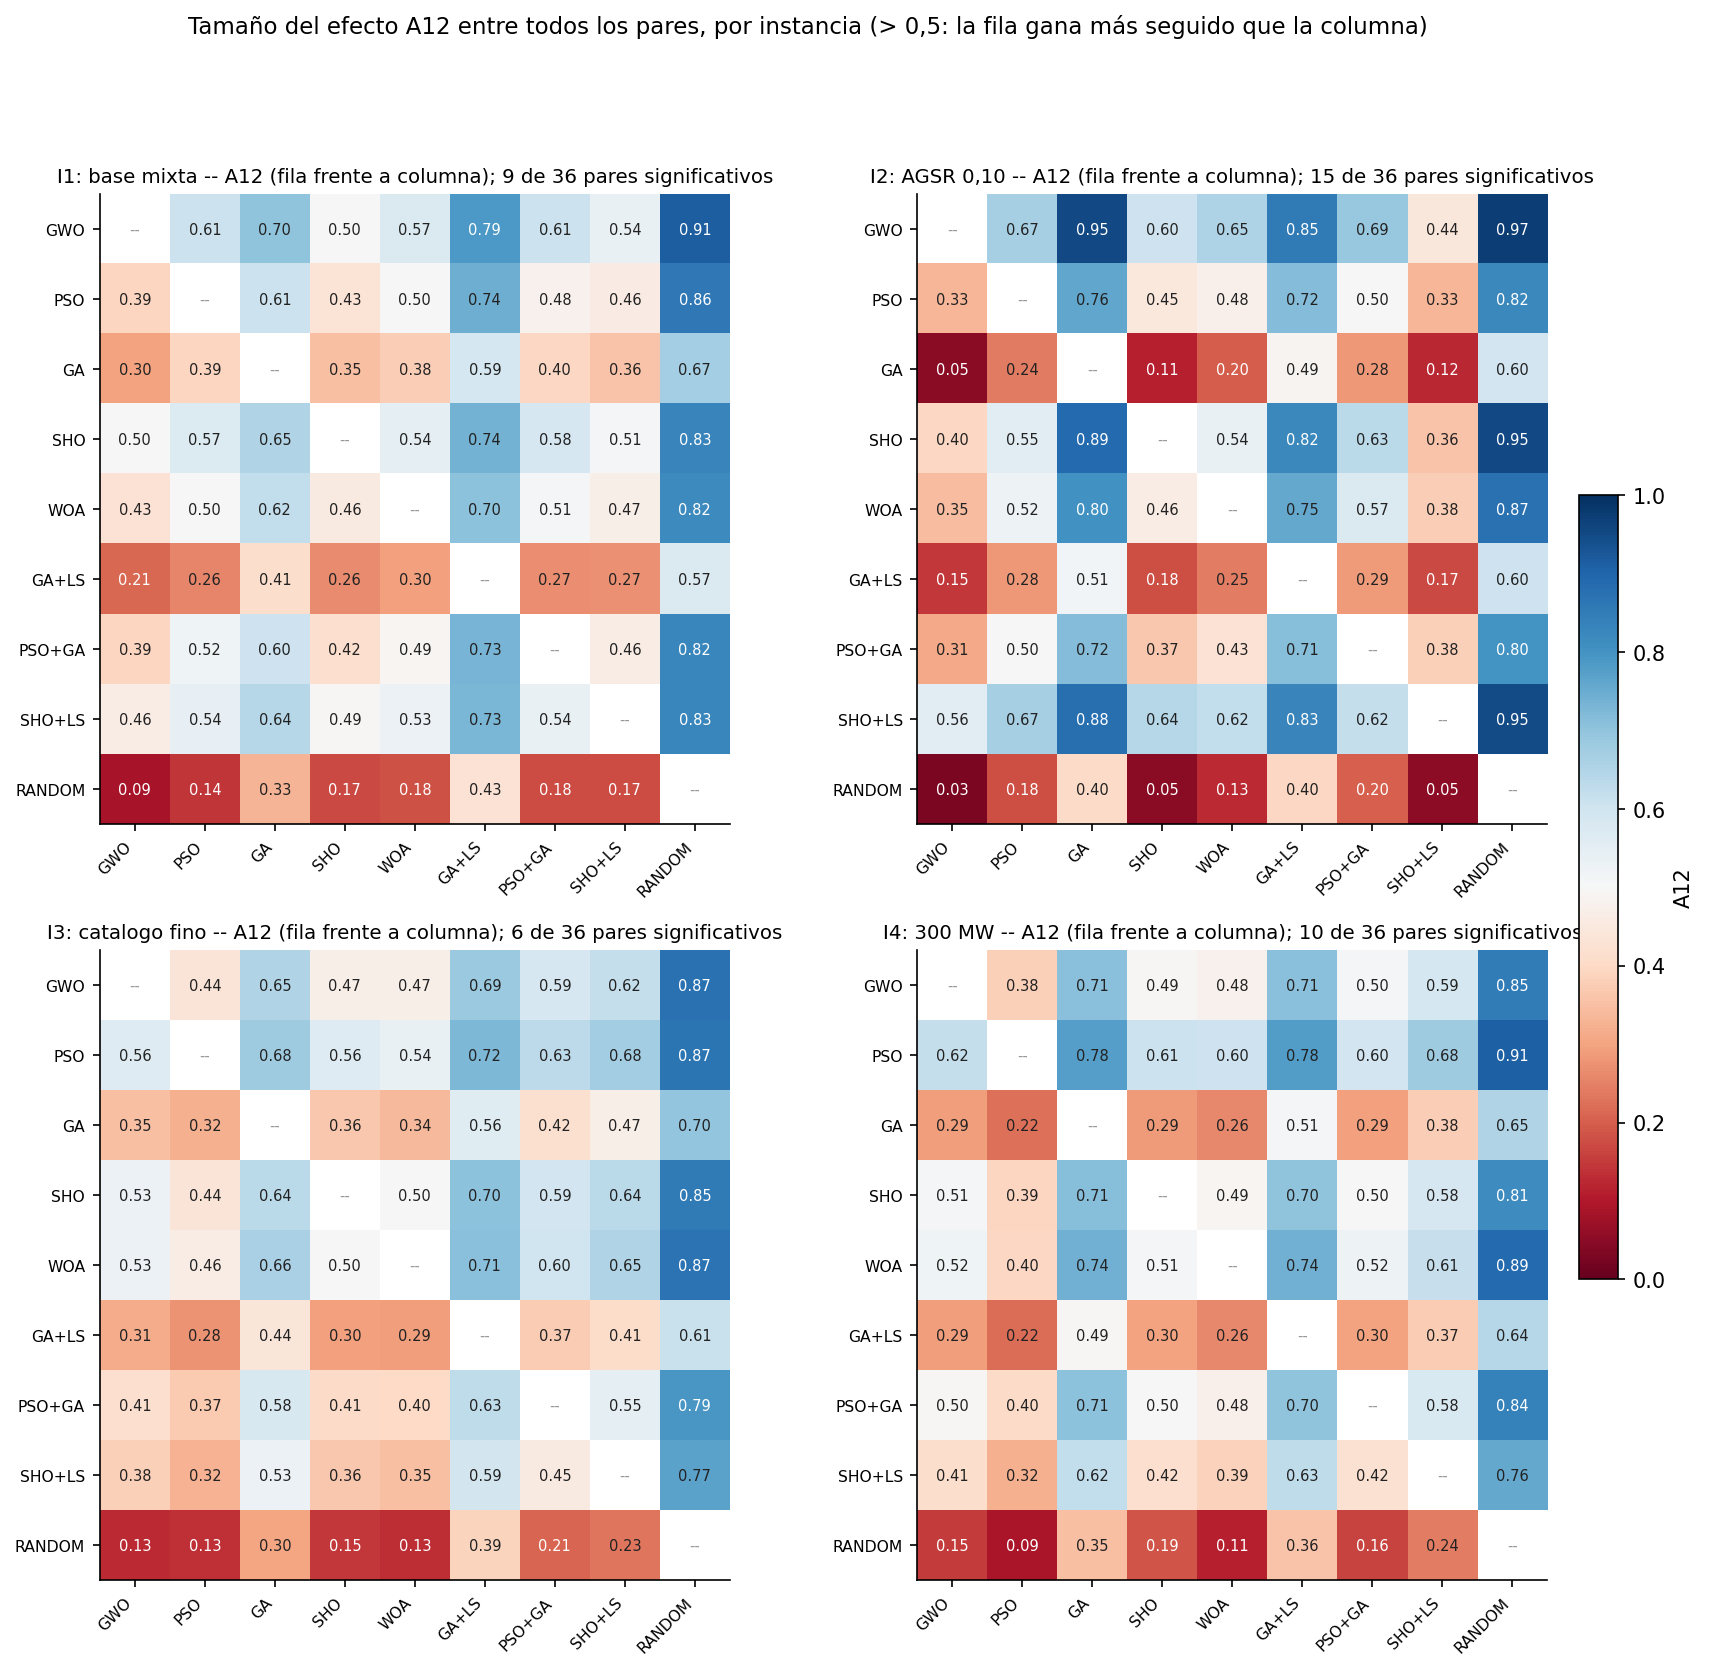
\includegraphics[width=0.98\textwidth]{figures/fig11_matrices_a12.png}
\caption{Tamaño del efecto $A_{12}$ entre todos los pares de algoritmos, por instancia. Valores mayores que 0,5 indican que la fila obtiene menor LCOE con más frecuencia que la columna.}
\label{fig:matrices_a12}
\end{figure}

\TablaParesCompletaAutoA
\TablaParesCompletaAutoB
\TablaParesCompletaAutoC
\TablaParesCompletaAutoD


\end{document}
